\documentclass[5p,times]{elsarticle}
% \documentclass[5p,twocolumn]{elsarticle}
%\documentclass[1p,onecolumn]{elsarticle}
\usepackage{lineno}
\usepackage{amssymb}
\usepackage{graphicx}
\usepackage{subcaption}
\usepackage{subcaption}
\usepackage{algorithm}
\usepackage{algpseudocode}
\usepackage{enumitem}
\usepackage{amsmath}
\usepackage{svg}
\usepackage{caption}
\usepackage{pifont}  % For checkmarks and crosses
\usepackage[protrusion=true,expansion=true]{microtype}
% \usepackage{placeins}  % For \FloatBarrier command
\usepackage{algorithm}
\usepackage{algpseudocode}
\usepackage{setspace}
\usepackage{booktabs}
\usepackage{caption}
\usepackage{adjustbox}


\journal{Future Generation Computer Systems}
\begin{document}
\begin{frontmatter}
\title{DiSIF: Distributed Semantic Information Fusion Framework for Smart City Applications}
\author{Ramin Rezvani-KhorashadiZadeh}
\ead{ra.rezvanikhorashadizadeh@mail.um.ac.ir}
\author{Mohsen Kahani\corref{cor1}}
\ead{kahani@um.ac.ir}
\address{Department of Computer Engineering, Ferdowsi University of Mashhad, Mashhad, Iran }
\cortext[cor1]{Corresponding author}
\begin{abstract}
  The advent of the Internet of Things (IoT) has accelerated the development of Digital Twins of Cities—virtual replicas of urban
 environments that enable real-time monitoring, analysis, and decision-making by integrating heterogeneous and high-velocity data
 streams from diverse sources. Managing these massive, heterogeneous data streams presents critical challenges including data
 fusion, scalability, privacy, and timely query execution. In this paper, we propose DiSIF (Distributed Semantic Information Fusion
 Framework), a novel architecture tailored for the Digital Twin of a City paradigm. DiSIF leverages semantic data models and
 RDF stream processing within a distributed semantic JDL fusion framework deployed across edge, fog, and cloud layers. This
 multi-layered design enables localized low-level data processing at the edge, significantly reducing raw data transmission and
 enhancing privacy. Horizontal fusion is performed by a multi-agent system (MAS) within each layer to improve processing speed and efficiency, while vertical fusion is conducted across distributed JDL layers to optimize bandwidth and computational resources.
  DiSIF also supports parallel execution of
 complex and dependent queries, substantially improving response times and resource utilization compared to centralized fusion
 models. Extensive evaluations in realistic urban scenarios demonstrate that DiSIF significantly enhances network efficiency, query
 performance, and scalability, making it a robust and scalable solution for implementing Digital Twins of Cities and advancing smart
 urban governance.

\end{abstract}
\begin{keyword}
semantic JDL, data fusion, fog computing, stream processing, RSP agent.
\end{keyword}
\end{frontmatter}
\section{Introduction}

Data fusion is a critical process in Digital Twins of Cities,
where multiple data sources from various applications need to
be integrated to improve decision-making and extract valuable
insights. Digital Twins of Cities represent virtual replicas of
urban environments that continuously ingest and analyze hetero
geneous data streams to provide real-time situational awareness
and predictive capabilities. By combining data from multiple
sensors, the limitations of individual sensors, such as range or
errors, can be overcome, resulting in enhanced system reliability
and broader situational awareness. Data fusion improves system
stability, increases accuracy, reduces uncertainty, and lowers
costs, all of which are essential for the complex and dynamic
nature of Digital Twin environments.

However, a major challenge in Digital Twins of Cities is
the heterogeneity of data sources. Data differences in syntax,
structure (schema), and meaning (semantics) can lead to issues
during fusion, creating semantic conflicts and reducing system
coherence. To address these challenges, a conceptual model
that provides a formal, common understanding of the target
domain is essential for successful data fusion in Digital Twin
environments.

The development and real-time maintenance of Digital Twins
 of Cities face substantial data-related challenges due to the massive,
  high-velocity, and heterogeneous nature of IoT sensor data
 streams. The immense data volume, such as traffic and weather
 streams producing many RDF triples per second, places
 significant computational demands on edge, fog, and cloud layers, straining resource scalability. The high velocity of these
 real-time streams requires rapid processing to ensure timely
 updates, essential for critical applications like traffic signal optimization. Moreover, data heterogeneity—stemming from diverse formats, schemas, and semantics across sources like traffic
 sensors and weather APIs—complicates integration, often resulting in semantic conflicts that undermine the accuracy and
 coherence of the Digital Twin. 
 
 To address the analytical challenges in Digital Twins of Cities, two critical issues must be tackled.
 First, heterogeneous concepts arise as many analyses require generating new data types distinct from raw sensor inputs,
  necessitating conceptual transformations to support query execution. For example,
   raw vehicle movement data must be transformed into higher-level concepts
    like congestion or traffic flow patterns. This is achieved through vertical fusion within
     a distributed JDL framework, where new concepts are created across distributed layers 
     (edge, fog, or cloud), ensuring semantic coherence and enabling advanced analytics.
      Second, the high-velocity data generated by IoT sensors, such as traffic or weather
       streams producing up to 10,000 RDF triples per second, demands a distributed infrastructure
        for scalable analytics. This is addressed through horizontal fusion within each layer,
         leveraging a multi-agent system (MAS) to enable parallel query execution, significantly enhancing processing speed and efficiency.
The Distributed Semantic Information Fusion Framework (DiSIF) addresses these challenges by integrating a three-layer
 (edge, fog, cloud) JDL-based architecture with Semantic Web technologies like RDF and SPARQL. By utilizing vertical 
 fusion across layers to create new concepts and horizontal fusion within layers for parallel query execution,
  DiSIF ensures efficient, scalable, and privacy-preserving data processing. This approach significantly improves query
   performance and resource utilization compared to traditional centralized models, making DiSIF a robust solution for
    operationalizing Digital Twins of Cities.

    Centralized data fusion models are inherently inefficient
    for large-scale Digital Twins of Cities due to several critical
    challenges. The massive data volumes generated by urban IoT
    sensors, such as traffic and weather streams, lead to network
    inefficiencies as all data must be transmitted to a single process
   ing node, causing bottlenecks and increased latency. Privacy
    concerns arise from the transmission of raw, sensitive data, such
    as vehicle GPS coordinates, to centralized servers, risking unau
   thorized access. Additionally, the high query execution times in
    centralized systems, particularly for complex semantic queries
    on large-scale RDF datasets, hinder real-time updates essential
    for applications like traffic management. The DiSIF framework addresses these limitations through a distributed architecture,
    concurrently across distributed nodes, with results com
   leveraging edge, fog, and cloud layers alongside Semantic Web
    technologies like RDF and SPARQL to enable scalable, privacy
   preserving, and low-latency data fusion for efficient urban Digi
   tal Twin operations.

   To overcome the challenges of data volume, velocity, and
   heterogeneity in Digital Twins of Cities, the DiSIF framework in
  troduces a distributed three-layer architecture comprising edge,
   fog, and cloud layers. This architecture enhances efficiency
   and scalability by processing high-volume, real-time IoT data
   streams locally at the edge layer, reducing network latency and
   preserving privacy. The fog layer handles complex semantic
   queries and data fusion, leveraging RDF and SPARQL to inte
  grate heterogeneous data, while the cloud layer supports macro
  level decision-making and historical analysis. By distributing
   computational tasks across these layers and employing paral
  lel query execution, DiSIF ensures scalable, low-latency, and
   privacy-preserving data fusion, meeting the demanding require
  ments of real-time urban Digital Twin applications.


  The JDL fusion model is a widely recognized model for data
  fusion, with its semantic version \cite{noughabi2013semfus} enabling the integration
  of heterogeneous data using Semantic Web technology such as
  RDFstream processing. This model can be implemented using
  centralized, distributed, or hybrid architectures. However, in
  Digital Twins of Cities, the traditional centralized semantic JDL
  model, where data is fused at a single node, faces challenges due
  to the vast data volume and the need for multi-layered decision
 making. This centralized approach is inefficient for large-scale
  data fusion, leading to increased response times, network in
 efficiencies, and costly decision-making processes, which are
  critical bottlenecks in real-time Digital Twin applications.

  To address these limitations, the DiSIF framework intro
  duces a three-layer architecture comprising edge, fog, and cloud
   layers. The edge layer handles time-sensitive decisions close
   to data sources, while the fog and cloud layers process more
   complex and macro-level decisions. This distributed architec
  ture aligns with the layered nature of Digital Twins of Cities,
   enabling scalable, privacy-preserving, and efficient data fusion
   and decision-making.


   Additional strengths of the DiSIF framework include:

   \begin{itemize}

   \item Execution of Independent Queries in Parallel: 
   
   Independent queries can be decomposed into sub-queries executed 
   concurrently across working agents within the multi-agent system (MAS) within layer,
    where agents collaborate to process sub-queries in parallel, 
    with results combined at master agent.

   This parallelism significantly optimizes query execution time, a crucial factor for real-time
 Digital Twin operations.

 \item Reduction of Network Load: By processing data locally
 and transmitting only processed results, DiSIF reduces
 network bandwidth utilization, addressing one of the main
 challenges in large-scale Digital Twin data management.
 
 \item Enhancement of Data Privacy: Local data processing
 avoids transmission of raw data, preserving privacy—a
 critical concern in urban Digital Twin deployments.

   \end{itemize}


   As stated earlier, the primary goal of this article is to present
 a distributed version of the semantic JDL fusion model tailored
 for Digital Twins of Cities. While various advancements have
 been made in different aspects of JDL fusion models, a fully
 distributed approach optimized for the scale, complexity, and
 real-time requirements of Digital Twins has not been explored
 until now. The innovations proposed in this article can be summarized as follows:

 \begin{itemize}
  \item Distributed Semantic JDL Fusion Model Across Three Layers (Edge, Fog, and Cloud)
  
  The Distributed Semantic Information Fusion Framework (DiSIF) implements
   a three-layer (edge, fog, and cloud) JDL fusion model to support hierarchical
    decision-making in Digital Twins of Cities. This architecture enables
     micro- and small-scale decisions at lower layers to be fused into macro-level 
     decisions at higher layers, aligning with the distributed nature of urban
      environments. DiSIF outperforms traditional centralized JDL fusion models
       by facilitating high-speed, parallel execution of decision-making processes
        across layers while separating fusion operations from decision-making tasks
         to enhance processing speed and manage complexity.
  \begin{itemize}
    \item Edge Layer: At the edge layer, Level-One fusion focuses
     on object refinement (as in JDL model), processing high-volume, real-time IoT data
      streams with low latency and privacy preservation.
       Key operations include RDFization and object refinement,
        enabling sensor fusion to integrate raw sensor
         data efficiently.
          A multi-agent system (MAS) is
          employed within this layer to perform parallel processing,
           ensuring rapid and localized data handling.
    \item Fog Layer: The fog layer conducts Level-Two fusion,
     emphasizing situation refinement (as in JDL model) to address complex semantic 
     queries. This layer performs data fusion, integrating
      and analyzing data to derive situational insights. The MAS within the 
      fog layer enables parallel execution of these queries,
       enhancing computational efficiency and scalability.
    \item Cloud Layer: In the cloud layer, 
    Level-Three fusion focuses on threat refinement (as in JDL model),
     synthesizing high-level insights for macro-level decision-making.
      The MAS within this layer supports parallel processing to
       manage complex computations effectively.
  \end{itemize}

  Across the three-layer JDL model, vertical fusion is performed 
  to transform concepts between layers, utilizing conceptOnto 
  to facilitate serial concept transformation from edge to fog to cloud.
   This ensures semantic coherence across layers,
    enabling seamless data integration. Within each layer, 
    the MAS drives parallel and independent fusion operations,
     significantly improving processing speed and scalability
      compared to centralized models, making DiSIF a robust solution
       for Digital Twins of Cities.


  \item Deployment of Multi-Agent System (MAS) in Each Layer
  In the DiSIF framework, each layer (edge, fog, and cloud) implements a segment of the
   JDL fusion model using a multi-agent system (MAS). Queries are decomposed into
    independent sub-queries, which are distributed to agents within the layer 
    for parallel execution. The results are then aggregated by a master agent,
     a process termed horizontal fusion. This approach enables efficient, 
     parallel processing of complex queries within each layer, significantly
      improving processing speed and resource utilization. By leveraging MAS 
      for horizontal fusion, DiSIF ensures localized, scalable data processing,
       making it well-suited for the high-volume, real-time data streams typical of Digital Twins.

  \item Introduction of ConceptOnto Ontology for Inter-Layer JDL Fusion.
  
  To enable high-level analytics in Digital Twins, complex queries at higher layers
   (e.g., cloud) must be rewritten into lower-level queries (e.g., edge or fog) 
   that align with the concepts available at those layers. The ConceptOnto ontology
    facilitates this query rewriting process by providing a structured framework for
     concept transformation across the distributed JDL layers. This vertical fusion 
     process ensures that outputs from lower-level queries are seamlessly propagated to
      higher layers, where they are fused according to the JDL model. The use of
       ConceptOnto enhances semantic coherence and enables accurate, hierarchical
        decision-making, making DiSIF a robust solution for advanced urban analytics.

 \end{itemize}


 It is important to note that while this article does not intro
 duce innovations specifically in the cloud domain, it leverages
  the cloud’s computational power for complex fusion tasks and
  macro-level decision-making within the Digital Twin framework.
  Decisions generated at the fog layer are forwarded to the cloud
  node for final aggregation and strategic urban management.


  The structure of the article is as follows: Section 2 reviews related
 works on data fusion models, Semantic Web approaches in smart
 cities, fog computing architectures, and RDF stream processing
 techniques. Section 3 details the DiSIF framework from the
 perspectives of the semantic JDL model and the proposed fusion
 , with a layer-by-layer discussion. Section 4 presents compre
hensive evaluations and analyzes the results. Finally, Section 5
 concludes the article. Additionally, the queries used in this study
 are provided in the Appendix A.

% The structure of the article is as follows: In section 2, related works on data fusion models, Semantic Web approaches
%  in smart cities, fog computing architectures, and RDF stream processing approaches are discussed. In section 3, the DiSIF framework is described from the perspectives of the JDL model and the fusion model. Each layer is then discussed separately. Evaluations are conducted from various perspectives and the results are analyzed in section 4 and the conclusion is presented in section 5. Additionally, 
% the queries used in this article are provided in the \ref{sec:AppendixQueries} .



\section{Related works}
This section reviews recent works for data fusion and analyzes various data fusion models. It also discusses studies that have utilized Semantic Web technologies in smart cities, explores fog computing architectures in smart city contexts, and reviews approaches to RDF stream processing.


\subsection{Data fusion methods}


% \begin{table*}[t]
% \centering
% \caption{Comparison of Activity Separation in Data Fusion Models}
% \label{tab:activity-separation}
% \begin{adjustbox}{max width=\textwidth}
% \begin{tabular}{@{}p{2.5cm}ccccccc@{}}
% \toprule
% \textbf{Model} & \textbf{Data Collection} & \textbf{Signal Processing} & \textbf{Object Refinement} & \textbf{Location Refinement} & \textbf{Threat Refinement} & \textbf{Decision Making} & \textbf {Acting} \\ 
% \midrule
% JDL Model & --- & Level0 & Level1 & Level2 & Level3 & Level4 & --- \\
% OODA Loop & Observe & Observe & Orient & Orient & Orient & Decide & Act \\
% Intelligence Cycle Model & Collection & Collection & Collection & Evaluation & Evaluation & Dissemination & Dissemination \\
% Omnibus Model & Sensing and Signal Processing & Sensing and Signal Processing & Feature Extraction & Decision Stage & Decision Stage & Decision Stage & Act Stage \\
% Object-Oriented Model & Actor & Actor & Perceiver & Perceiver & Perceiver & Director & Manager \\
% \bottomrule
% \end{tabular}
% \end{adjustbox}
% \end{table*}



The process of data and information fusion involves combining inputs to create richer information than what can be obtained from
 each input separately. 





One of the common models in the field of fusion is the multi-level JDL model \cite{Hall1997},
 which with its 5 different levels covering from raw data processing to decision-making, has contributed to the comprehensiveness and popularity of this model in the fusion domain.


% \begin{table}[t]
%   \centering
%   \caption{Comparison of Data Fusion Models based on Data, Model, and Data Fusion Type}
%   \label{tab:data-fusion-models}
%   \begin{adjustbox}{max width=\columnwidth} % Adjust to fit in one column
%   \begin{tabular}{@{}llll@{}}
%   \toprule
%   \textbf{Data} & \textbf{Model} & \textbf{Data Fusion Type} & \textbf{Situation/Threat Refinement} \\ 
%   \midrule
%   JDL Model              & Data-Based       & Shared Memory (BUS)   & \ding{51}  \\
%   OODA Loop              & Activity-Based   & Sequential            & \ding{55}  \\
%   Intelligence Cycle Model & Activity-Based  & Sequential            & \ding{55}  \\
%   Omnibus Model          & Activity-Based   & Sequential            & \ding{55}  \\
%   Object-Oriented Model  & Role-Based       & Sequential            & \ding{55}  \\
%   \bottomrule
%   \end{tabular}
%   \end{adjustbox}
%   \end{table}
  




\begin{figure}[t]
  \centering
  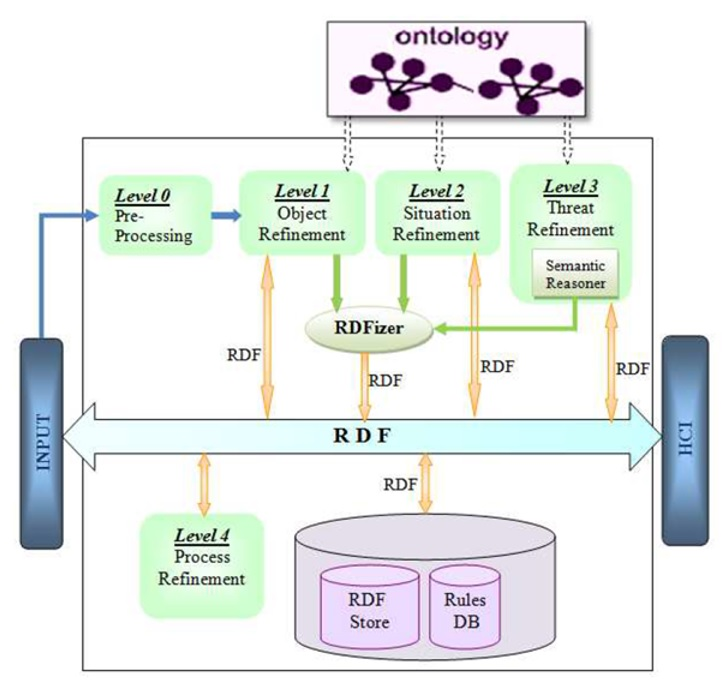
\includegraphics[width=\columnwidth]{Semantic_JDL.jpg}
  \caption{The semantic JDL model \cite{noughabi2013semfus}}
  \label{fig:semantidJDL}
\end{figure}


The semantic JDL model \cite{noughabi2013semfus} combines the basic JDL model with Semantic Web technologies.
The JDL semantic model in Figure \ref{fig:semantidJDL} is structured into several levels, each addressing different aspects of data processing. At Level 0, the focus is on preprocessing various data sources, resulting in cleaned data that is forwarded for object refinement without introducing any semantic elements. Level 1 involves transforming objects and their attributes into standard RDF format for storage. While this level includes tasks such as object identification, these processes rely on mathematical algorithms and image processing rather than semantic definitions. To effectively structure the data, predefined ontologies are necessary, allowing for the integration of attributes into the RDF format using an RDFizer, with the data stored in an RDF-Store database.
In Level 2, the model uses prior knowledge and environmental information alongside RDF data from Level 1 to define the situation of objects and their interrelationships. New relationships and previously unknown attributes are identified through inference, leading to updates in the RDF data that reflect any changes in information.
Level 3 emphasizes the evaluation of the current situation and the prediction of potential threats and vulnerabilities. A semantic reasoner plays a crucial role at this level, employing inference techniques to assess the situation and identify solutions and opportunities related to threats. The results of this analysis are converted into RDF format for storage.
Finally, Level 4 focuses on monitoring the system's performance and resource allocation. An expert evaluates the outputs from Level 3 to make informed decisions that enhance the overall efficiency of the system. The JDL semantic model operates with multiple databases, including one for RDF information and ontologies and another for rules. Proper database management principles must be upheld to ensure compatibility, prompt updates, and efficient data handling. Specific details regarding inputs and outputs may vary based on the domain of application.

One of the notable features of JDL, which makes it suitable for distributed architecture, is its ability to effectively separate tasks.
One of the advantages of the JDL fusion model over other fusion models is the separation of fusion stages into completely
distinct parts. This allows for the distribution of different components of the JDL model across various systems, 
enabling distributed fusion operations. 
Therefore, in this article, the JDL fusion model is utilized to present its distributed version 
for smart traffic application.


\subsection{Semantic Web in smart city}

Architectures of smart cities should combine data received from sensors in a manner that is readable by machines and publishable. To add meaning to the raw data generated by sensors and enhance data interaction and integration, Semantic Web technology has been employed. Semantic Web adds new information to the architectures of Internet of Things (IoT) for sensor fusion.



In \cite{article28}, the LSM architecture is introduced to achieve data interaction through the Semantic Web by integrating sensor data. It provides a user interface for publishing, annotating, and querying sensor data, utilizing the SSN ontology for describing sensor data and streams. The architecture links time-dependent data with external resources through semantic annotations, standardizes diverse data formats, and incorporates contextual knowledge from sources like DBpedia and GeoNames to enhance advanced querying.
This approach does not address query decomposition and distributed query execution and does not consider
  optimizing query execution. Additionally, it considers the execution of CQELS queries centrally and does not consider 
  the cost of sending data to the central node.


In \cite{Al-Baltah2020}, the SDFF framework is proposed to integrate data from heterogeneous sensors using Semantic Web technologies to resolve inconsistencies, such as differences in measurement units. It consists of layers for raw data collection, storage (separate repositories for raw and semantic data), semantic annotation, conflict resolution, and data dissemination. The framework ensures accurate data fusion and comparison, offering a comprehensive solution for managing and harmonizing diverse sensor data.
This article does not discuss topics such as distributed processing and query execution, query execution optimization, processing of large streaming data, and prevention of sending data to only one central node (centralized approach).


In \cite{Samadian2014}, a framework is introduced to combine and aggregate heterogeneous data streams from sensors, 
transforming them into feature streams to reduce data volume and increase efficiency.
 In \cite{inproceedings31}, sensor data is converted into RDF based on domain ontologies, 
 focusing on reducing transmitted data and optimizing bandwidth, but it lacks discussion on query 
 processing and execution optimization.
  In \cite{article32}, the Sense2Web framework enhances data integration by semantically representing sensor features and linking them to external resources, facilitating seamless aggregation and system interaction.


In \cite{inproceedings33}, a novel architecture is introduced for aggregating heterogeneous sensor networks
 by converting sensor measurements into semantic data and using ontologies for 
 enhanced data aggregation. However, it does not cover a distributed three-layer 
 architecture for data collection, query processing, or bandwidth management.
  In \cite{Wang2017}, another architecture integrates heterogeneous IoT data with a
   data aggregation layer to unify and improve data quality. Although it enhances 
   data fusion at a central node, it lacks an optimized query processing model and 
   a distributed approach that could improve system performance.


The SIGHTED architecture \cite{article35} collects and disseminates sensor data but faces challenges due to its
 centralized approach. Annotated data is stored and queried later, which increases query response times. 
 Drawbacks include lack of query optimization, inability to handle large data streams, 
 and reliance on sending all data to a central node. In \cite{Zafeiropoulos2008},
  a semantic framework with three layers—data collection, processing, and a semantic 
  layer—ensures data consistency and annotation through ontologies. However, it lacks
   distributed processing and centralizes data, leading to inefficient query execution
    and no optimization for large data transmission. In \cite{belcao2020streaming}, 
    a framework utilizing Streaming Virtual Knowledge Graphs integrates semantic data 
    streams using OBDA. While effective for data integration, generating ontologies from
     RDBMS databases is time-consuming and inefficient for decentralized environments 
     like smart cities, lacking efficient query decomposition and execution capabilities.



In \cite{zappatore2023semantic}, the study addresses semantic interoperability challenges
 in smart cities where diverse IoT solutions generate large data volumes exchanged via APIs. 
 It highlights the role of ontologies and shared vocabularies to enhance environmental sensing 
 and wellness monitoring. By using sensor-agnostic APIs and ontology modules for mobile crowd-sensing,
  the framework improves data integration, scalability, and real-time responsiveness in IoT applications.
   Privacy concerns in smart cities are addressed by the 'Ontology-Based Privacy-Preserving' (OBPP) framework \cite{GHEISARI20211},
    which uses ontologies and semantic reasoning to tackle heterogeneity, privacy, and service provision.
     Additionally, Semantic Web technologies play a key role in Agriculture 5.0 by improving data interoperability, 
     accessibility, and real-time operations in the agricultural sector \cite{de2023spatio}.    





\subsection{Fog Computing architectures}


Cloud computing offers extensive resources for handling complex tasks in smart cities \cite{Garca2011ExploringTL},
 but it has limitations such as high latency, lack of contextual awareness, and inadequate mobility support,
  which impede real-time processing. Edge computing addresses these issues by extending cloud capabilities to 
  the network edge, providing localized processing and storage to reduce latency and improve bandwidth efficiency,
   making it ideal for real-time smart city services \cite{Ahmed2017BringingCC}, \cite{Rahman2019BlockchainAI}.
    Additionally, cloud and fog computing are explored to bring cloud resources closer to the edge,
     enhancing the performance of smart city systems \cite{Abbas2018MobileEC}.




Perera \cite{Perera2017FogCF} explores real-world fog computing applications in agriculture, healthcare, and transportation
 but does not cover Semantic Web-based approaches. In \cite{Hu2017SurveyOF}, fog and edge computing are compared with cloud computing
  in smart environments, focusing on privacy, energy consumption, and challenges, but without integrating Semantic
   Web solutions. Shi \cite{Shi2016EdgeCV} highlights the benefits and challenges of edge computing, including privacy 
   and service optimization, through case studies, but lacks Semantic Web integration. Recent research on fog 
   computing and the Internet of Everything (IoE) \cite{Baccarelli2017FogOE} addresses latency reduction and 
   resource constraints, emphasizing scalability and real-time capabilities but provides limited detail on
    smart city applications. In \cite{Giordano2016SmartAA}, a three-layer architecture called Rainbow
     uses intelligent agents in smart city IoT systems but omits Semantic Web technology for data fusion.
      In \cite{inproceedings61}, a tiered-edge architecture introduces semantic stream processing 
      for workload distribution but lacks ontology-based query decomposition and efficient sub-query handling.


 
FogBus \cite{TULI201922} is a framework for cloud-fog integration, improving performance by 
activating cloud resources during overload, but it lacks semantic data processing and query 
decomposition. The "Analytics Everywhere" architecture \cite{article63} uses edge, fog, and cloud layers
 for smart parking analytics but does not optimize user requests or use RDF for data fusion. A four-layer
  fog architecture \cite{Arkian2017} focuses on context awareness and low latency but 
  lacks Semantic Web and data fusion models. Dastjerdi's five-layer architecture \cite{Dastjerdi2016} misses a distinct 
  fog layer and fails to address semantic issues. In \cite{ortiz2022atmosphere}, a collaborative IoT architecture using agent-oriented algorithms
   and CEP does not support semantic or heterogeneous data processing. A CR edge processing platform \cite{bonte2023towards} improves
    cloud efficiency but lacks high-level query translation and load balancing strategies. Recent studies \cite{XHAFA2020730} highlight edge computing’s role
     in enhancing data quality through semantic enrichment and event processing in smart cities. To address data integrity challenges in fog computing, \cite{SELLAMI202464} 
     introduces a verification protocol using SIS and identity-based signatures, improving security and efficiency.



\subsection{RDF stream Processing appoaches}


Real-time processing of large data streams has led to the development of RDF stream processing (RSP) models
 and continuous querying languages aimed at addressing the challenge of heterogeneous data. Systems such
  as EP-SPARQL \cite{anicic2011ep}, SPARKWAVE \cite{komazec2012sparkwave}, and INSTANS \cite{rinne2012instans} utilize temporal operators,
   while others like C-SPARQL \cite{barbieri2010c} and CQELS \cite{le2011native} rely on sliding windows for continuous query execution.

RSP system implementations are generally categorized into distributed and centralized models. Distributed approaches, such as DRSS \cite{dia2018drss},
 built on the Apache Storm platform, and CQELS Cloud \cite{le2013elastic}, leverage frameworks like Spark Streaming,
  Flink, and Storm for parallel stream processing. While these models enhance scalability and parallel execution,
   they often introduce complexities in implementation, upgrading, and usage. Centralized models, including
    C-SPARQL \cite{barbieri2010c}, SparqlStream \cite{calbimonte2010enabling}, and SPARKWAVE \cite{komazec2012sparkwave}, 
    struggle with processing capacity and exhibit limitations in scalability, concurrent query handling, and collaboration.


MAS4MEAN \cite{mebrek2020stream} addresses the limitations of centralized models by adopting a multi-agent approach that parallelizes query processing 
through multiple instances of the C-SPARQL engine.
Despite its ability to manage large event volumes,
   MAS4MEAN faces challenges in accelerating complex queries, performing local query execution,
    and avoiding redundant sub-query execution, leading to bandwidth inefficiency and increased query times as data and query complexity grow.

While continuous query operators for SPARQL 
have been developed to address stream heterogeneity, challenges related to parallelization and scalability persist.
 Methods such as DIONYSUS \cite{gillani2016dionysus} and CQELS Cloud \cite{le2013elastic} focus on distributing and processing large-scale RDF
  streams in parallel. Efficient partitioning of queries and data across nodes, with minimal data exchange, remains essential for
   optimizing the processing of RDF data streams at scale.



The article \cite{dia2018drss} introduces a scalable distributed approach for RDF stream processing by
 leveraging query rewriting, partitioning, and RDF graph partitioning to minimize inter-node data exchange.
  However, it lacks a task assignment strategy and does not implement a master-worker framework, leaving some execution details unclear.

The Waves method \cite{khrouf2016waves} utilizes the Apache Storm framework to distribute C-SPARQL
 queries across nodes, effectively handling large data volumes. However, it does not incorporate query 
 decomposition, leading to redundant executions and inefficient query performance.

StreamQR \cite{calbimonte2016query} rewrites C-SPARQL queries into a Union of Conjunctive Queries (UCQ)
 based on ontology, injecting domain knowledge into the query. While this allows parallel execution, 
 it can create large queries with multiple unions, increasing execution costs without optimizing time window lengths or conditions.

Table \ref{tab:comparison} outlines various frameworks and their capabilities, including query decomposition, 
prevention of redundant query execution, and whether they employ a layered architecture.
 The DIVIDE platform \cite{de2024enabling} dynamically adapts IoT stream queries based on real-time contexts
  using Semantic Web technologies but focuses mainly on dynamic query adaptation, leaving some performance aspects dependent on network conditions.



%\onecolumn

\begin{table*}[h!]
  % \centering
  % \flushleft % Align the caption to the left
  % \caption*{\textbf{Summary of related works}} % Use caption* to remove the extra space
  % \caption{Summary of related works}

  % \caption{\hspace{-\leftmargin}Summary of related works} % Adjust horizontal position
  % \vspace{-0.5em} % Adjust vertical space to remove blank lines

  \captionsetup{justification=raggedright, singlelinecheck=false} % Left-align the caption
  \caption{\newline Summary of related works}
  \vspace{-1em} % Adjust this value to remove blank space if necessary



  \resizebox{\textwidth}{!}{%
  \begin{tabular}{lccccccc}
    \hline
      \textbf{Method} & \textbf{Query Decomposition} & 
      \textbf{Duplicate Query Execute} & \textbf{Handle Large Data Stream} &
       \textbf{Query Processing} & \textbf{DataType} & \textbf{Layered Architecture} &
       \textbf{Query Optimization}  \\ \hline
       Zafeiropoulos et al. 2008 \cite{Zafeiropoulos2008} & \ding{55} & - & \ding{55} & C & RDF & \ding{51} & \ding{55}  \\ 
       Patni et al. 2011 \cite{inproceedings31} & \ding{55} & - & - & C & RDF & \ding{55} & \ding{55}  \\ 
       De et al. 2012 \cite{article32}  & \ding{55} & - & - & C & RDF & \ding{55} & \ding{55}  \\ 
      Phuoc et al. 2012 \cite{article28} & \ding{55} & - & - & C & RDF & - & \ding{55}  \\ 
      Gyrard et al. 2013 \cite{inproceedings33} & - & - & - & C & RDF & \ding{55} & -  \\ 
      Nagib et al. 2016 \cite{article35} & \ding{55} & - & \ding{55} & C & RDF & \ding{55} & \ding{55}  \\ 
      Dastjerdi et al. 2016 \cite{Dastjerdi2016} & - & - & - & C & Non-RDF & \ding{51} & -  \\ 

      Giordano et al. 2016 \cite{Giordano2016SmartAA} & - & - & - & - & Non-RDF & \ding{51} & -  \\ 
      Khrouf et al. 2016 \cite{khrouf2016waves} & \ding{55} & \ding{51} & \ding{51} & D & RDF & \ding{55} & \ding{55}  \\ 
      Calbimonte et al. 2016 \cite{calbimonte2016query} & Syntactically & \ding{51} & \ding{51} & C & RDF & \ding{55} & \ding{55}  \\ 

      Wang et al. 2017 \cite{Wang2017} & \ding{55} & - & - & C & RDF & \ding{51} & \ding{55}  \\ 
      Arkian et al. 2017 \cite{Arkian2017} & \ding{55} & - & \ding{51} & D & Non-RDF & \ding{51} & \ding{55}  \\ 
      Dia et al. 2018 \cite{dia2018drss} & Syntactically & \ding{55} & \ding{51} & D & RDF & \ding{55} & \ding{51}  \\ 

      Tuli et al. 2019 \cite{TULI201922} & \ding{55} & - & \ding{51} & D & Non-RDF & \ding{51} & \ding{55}  \\ 
      Cao et al. 2019 \cite{article63} & \ding{55} & \ding{51} & \ding{51} & D & Non-RDF & \ding{51} & \ding{55}  \\ 

      Al-Baltah et al. 2020 \cite{Al-Baltah2020} & \ding{55} & - & - & C & RDF & - & \ding{55}  \\ 
      Mebrek et al. 2020 \cite{mebrek2020stream} & \ding{55} & \ding{51} & \ding{51} & D & RDF & \ding{51} & \ding{55}  \\ 

      Ortiz et al. 2022 \cite{ortiz2022atmosphere} & \ding{55} & - & - & D & Non-RDF & \ding{51} & \ding{55}  \\ 
      Bonte et al. 2023 \cite{bonte2023towards} & Syntactically & - & \ding{51} & D & RDF & \ding{51} & \ding{51}  \\ 
      \textbf{DiSIF (our solution)} &   \textbf{Semantically} & 
      \textbf{\ding{55}} &   \textbf{\ding{51}} &   \textbf{D} &   \textbf{RDF} &   \textbf{\ding{51}} &
      \textbf{\ding{51}}  \\ \hline
  \end{tabular}
}
  
  \label{tab:comparison}
  \vspace{1mm} % Optional: add space before the note
  \footnotesize{Note: C and D refer to "Centralized" and "Distributed", respectively}
\end{table*}




% \begin{figure*}
%   \centering

%   \includegraphics[width=0.5\textwidth]{AllinOneFrameWork_modified.drawio.pdf}
%   \caption{DiSIF framework}
%   \label{fig:overall}
% \end{figure*}

\begin{figure}[t]
  \centering
  % \includegraphics[width=\columnwidth]{AllinOneFrameWork_modified.drawio.pdf}
  \includegraphics[width=\columnwidth]{AllinOneFrameWork_modified.drawio.pdf}
  \caption{DiSIF framework}
  \label{fig:overall}
\end{figure}

%\twocolumn



%???????????????????????? end related workd ??????????????????





\section{DiSIF: Distributed Semantic Information Fusion framework}


In this section, we introduce the distributed version of the
semantic JDL model within the framework of a three-layer architecture—edge,fog,and 
cloud— specifically designed to support
the complex and dynamic data environment of a Digital Twin
of a City. As a case study, we apply this model to the traffic
detection problem, a critical use case in urban digital twins for
real-time monitoring and management.







\begin{figure*}
    \centering
  
    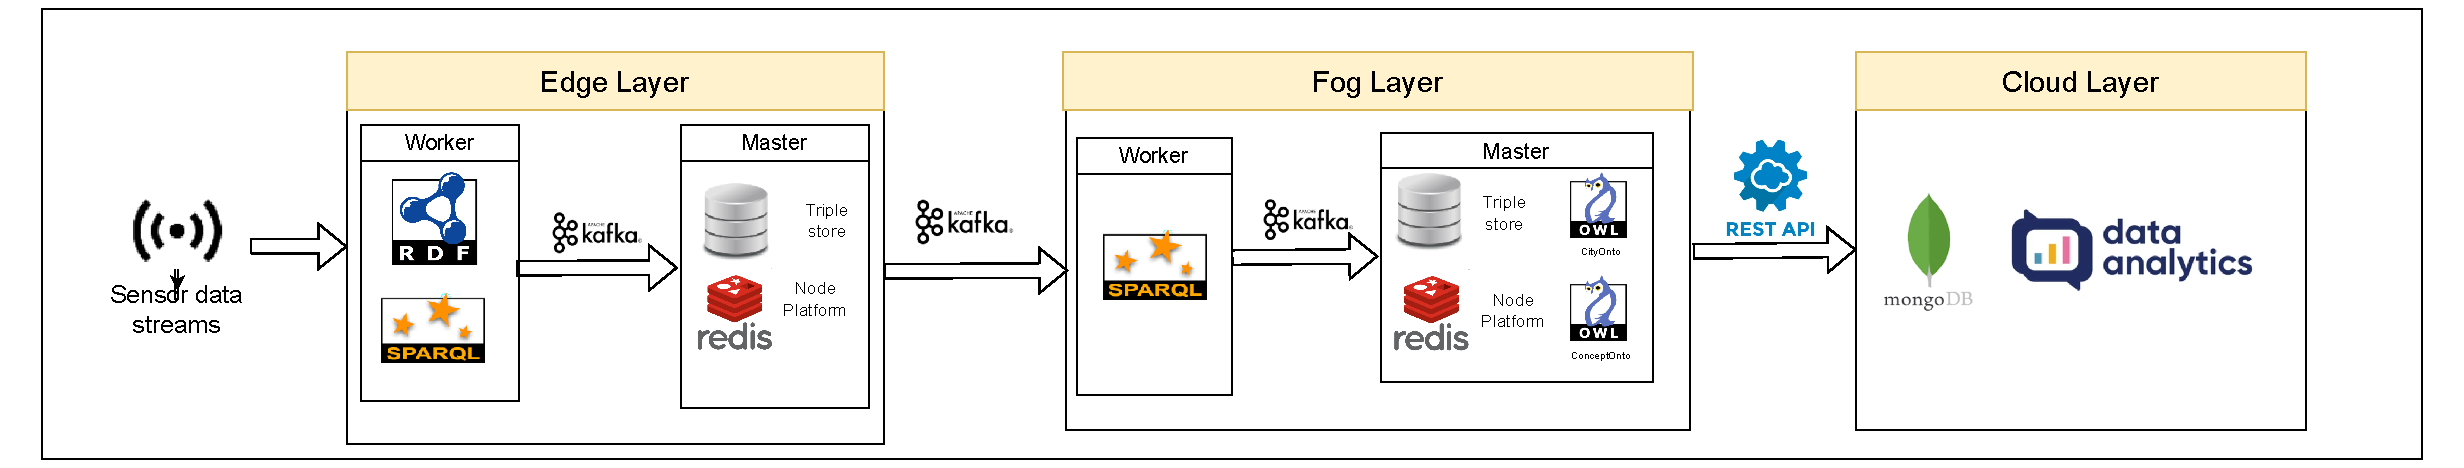
\includegraphics[width=1\textwidth]{Overall_Framework_Communication_OK.drawio.pdf}
    \caption{DiSIF Communication}
    \label{fig:overall_communication}
  \end{figure*}


\subsection{Overview of DiSIF Framework}

The DiSIF framework consists of three
 hierarchical layers—edge, fog, and cloud—engineered
  to facilitate both time-sensitive and complex dependent decision-making processes in
  IoT applications that underpin Digital Twins of Cities. This layered design enables progressive
   data processing and fusion aligned with the multi-scale and multi-domain nature
    of urban digital replicas. We analyze the DiSIF framework’s layers from two 
    complementary perspectives: the semantic JDL fusion model and the fusion process itself.


\subsubsection{The JDL model perspective}

As illustrated in Figure \ref{fig:JDLandFusionprespective},
 the DiSIF framework is organized into three layers: edge, fog, and cloud. Each layer
 comprises two types of nodes: worker nodes and master nodes.
  Worker nodes are responsible for receiving and performing
   initial processing on data streams collected from physical sensors
    or lower layers. The processed results are then transmitted to the
     corresponding master nodes for further fusion and decision-making.

At the edge layer, DiSIF performs the first level of processing,
 known as object refinement, which involves real-time, resource-efficient operations with minimal
  latency. This layer is critical in the Digital Twin context for immediate, 
  localized decision-making, such as detecting individual vehicles or traffic incidents.
   The tasks at this layer align with the object refinement component of the semantic JDL model.

Decisions and fused information from the edge layer are forwarded to 
the fog layer for the second level of processing, called situation refinement.
 Here, more complex and aggregated decisions are made, such as identifying traffic
  congestion patterns or emergent urban events. The fog layer utilizes the cityOnto ontology
   to semantically integrate and aggregate data, enabling richer context-aware decision-making 
   that reflects the evolving state of the Digital Twin.

Finally, for comprehensive, city-wide analysis and strategic decision-making, 
the aggregated data and intermediate results from the fog layer are sent to the cloud layer.
 This layer corresponds to the third level of the JDL model, known as threat refinement
  or macro-level decision-making. The cloud layer maintains a centralized database storing all
   processed information and executes intensive computational tasks, including long-term traffic
    pattern prediction, anomaly detection, and policy-level urban management decisions.
     Thus, data processing, fusion, and decision-making occur progressively and hierarchically 
     across the DiSIF layers, reflecting the multi-scale nature of the Digital Twin of a City.






%\begin{figure*}
%  \centering
%  \includegraphics[width=0.8\textwidth]{C:/Users/Administrator/Desktop/Thesis_latex_Final/AllinOneFrameWork_modified.drawio.pdf}
%  \caption{The JDL model perspective}
%  \label{fig:framework1}
%\end{figure*}  




% In this section, we first address the definition of the concepts of independent queries and dependent queries.
% \begin{itemize}
%  \item \textbf{Independent Query} 

% An independent query in C-SPARQL is a query that can be executed without dependence on the results of other queries. Additionally, it can be decomposed into independent subqueries, which can be executed in parallel without any interdependency, enabling efficient and scalable data processing. The results of these subqueries are separate from each other and can be executed and obtained without any connection to each other. An example of such a query is to investigate the number of vehicles present in a specific area. This query can be divided into subqueries that count the number of vehicles on the streets within that area. Each subquery can be executed independently, and the results can be published separately.

%     \item \textbf{Dependent Query}

%  A dependent query in C-SPARQL is a query that relies on the results of one or more previous C-SPARQL queries for its execution. Dependent C-SPARQL queries are usually used to perform operations such as analysis or further processing on the results of previous queries. This is essential for complex data analysis tasks involving sequential or fusion operations on RDF data streams.

% \end{itemize}

\begin{figure}[t]
    \centering
    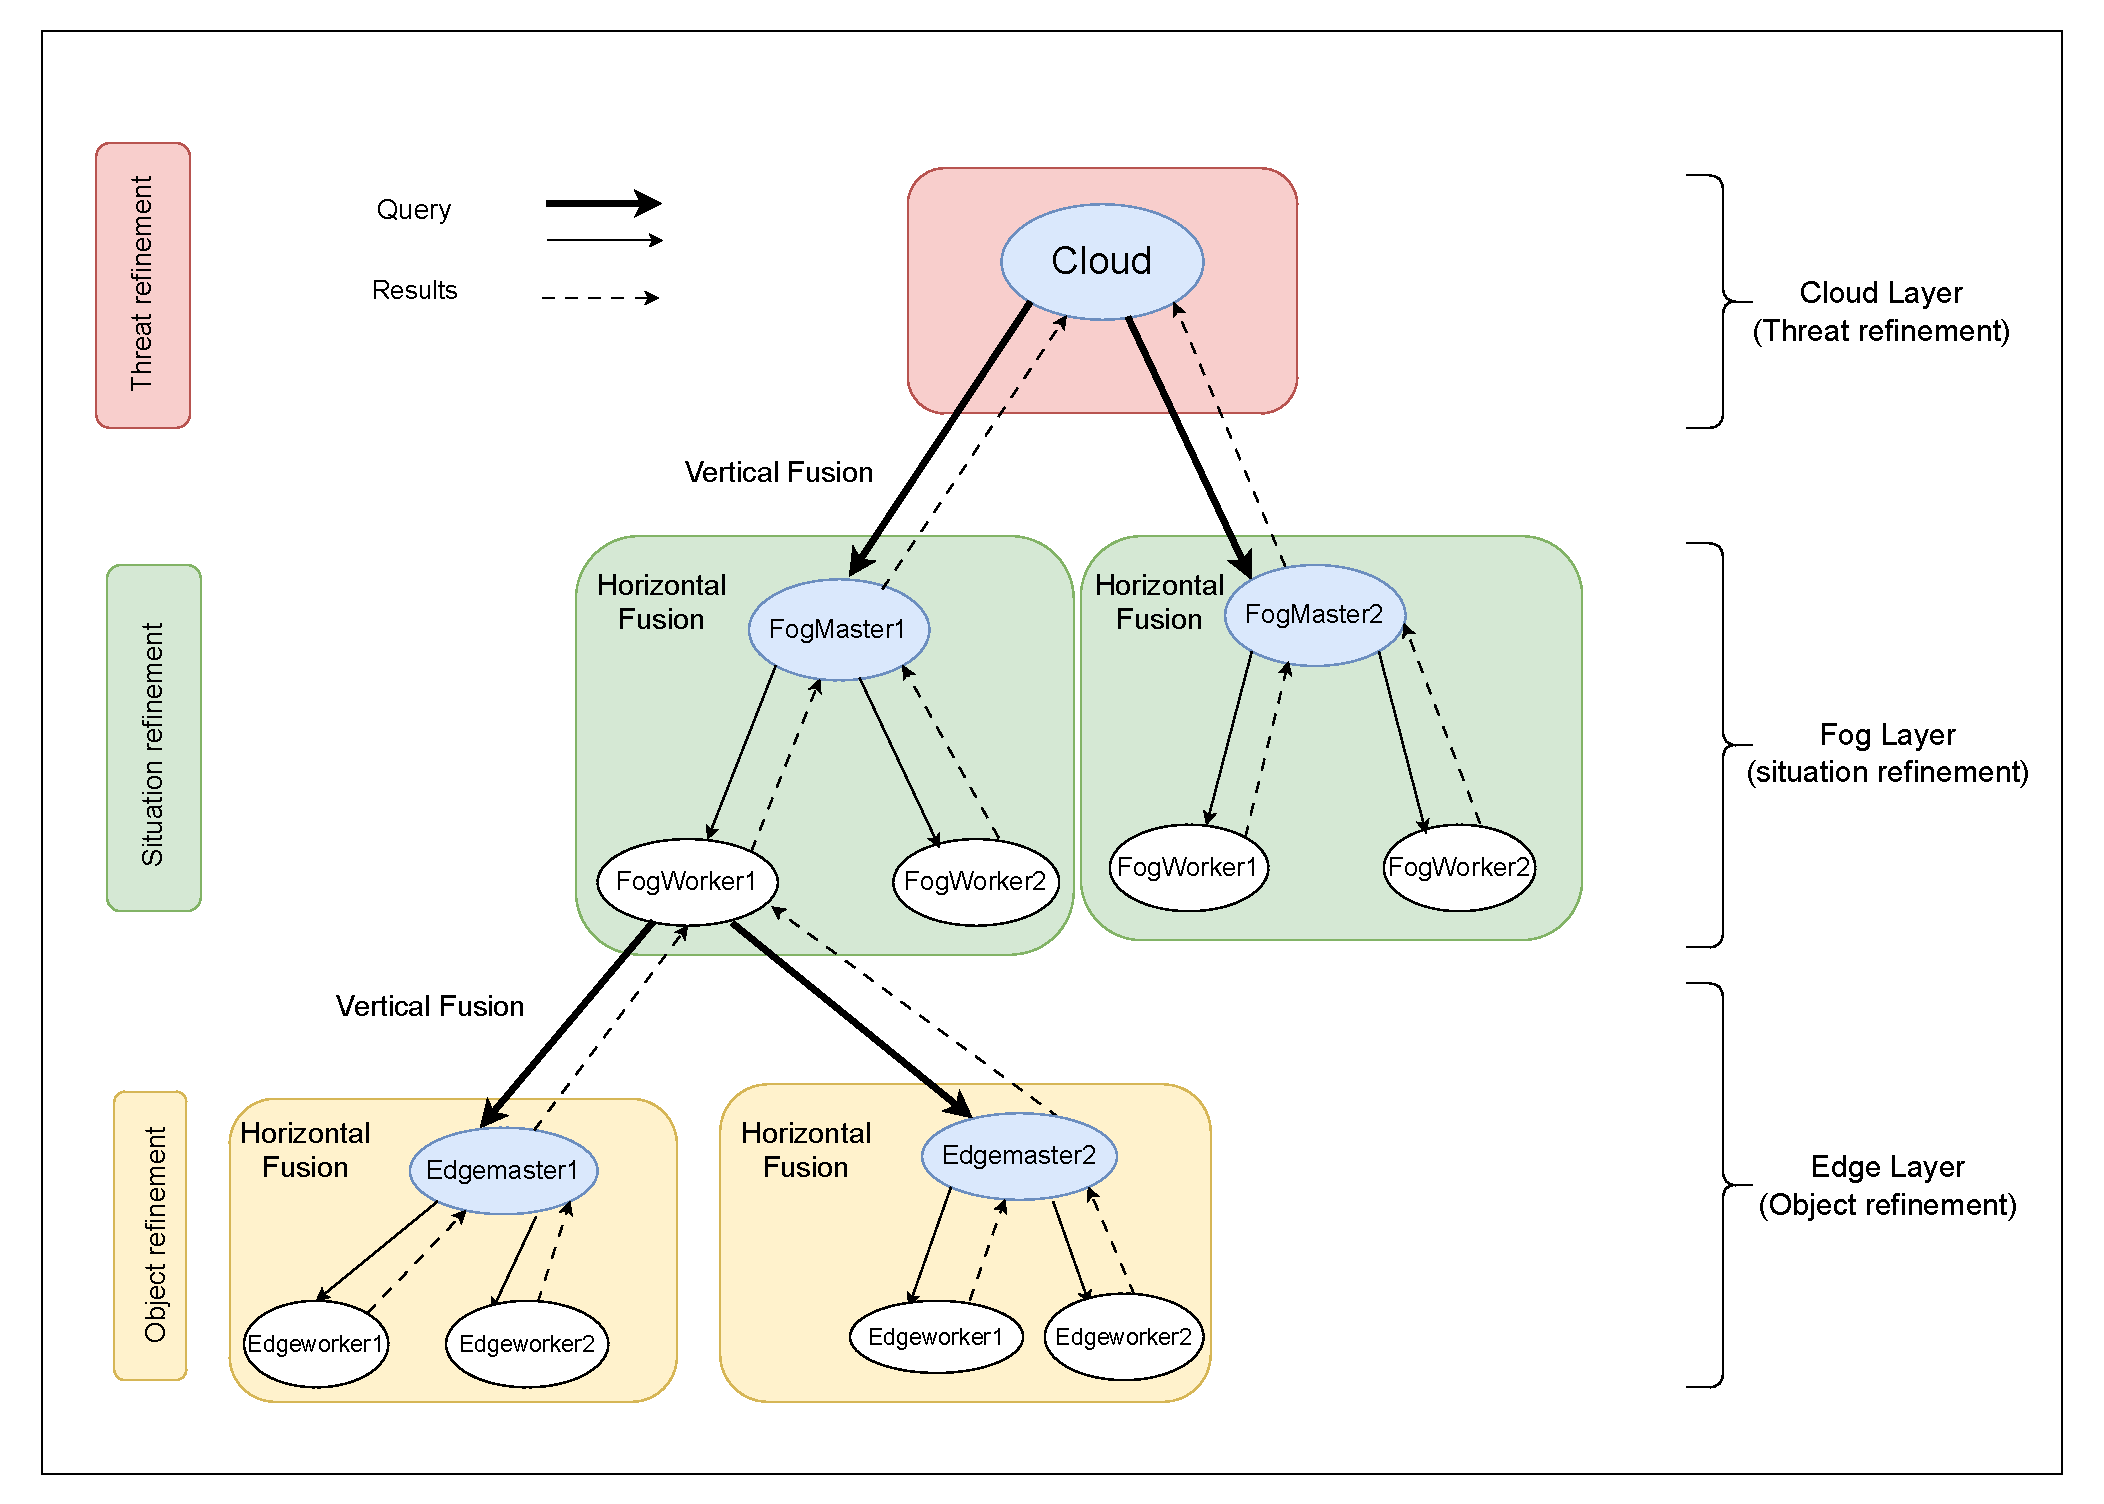
\includegraphics[width=\columnwidth]{h3_new.drawio.pdf}
    \caption{The JDL and fusion model perspectives}
    \label{fig:JDLandFusionprespective}
  \end{figure}

  
% \begin{figure*}
%   \centering
%   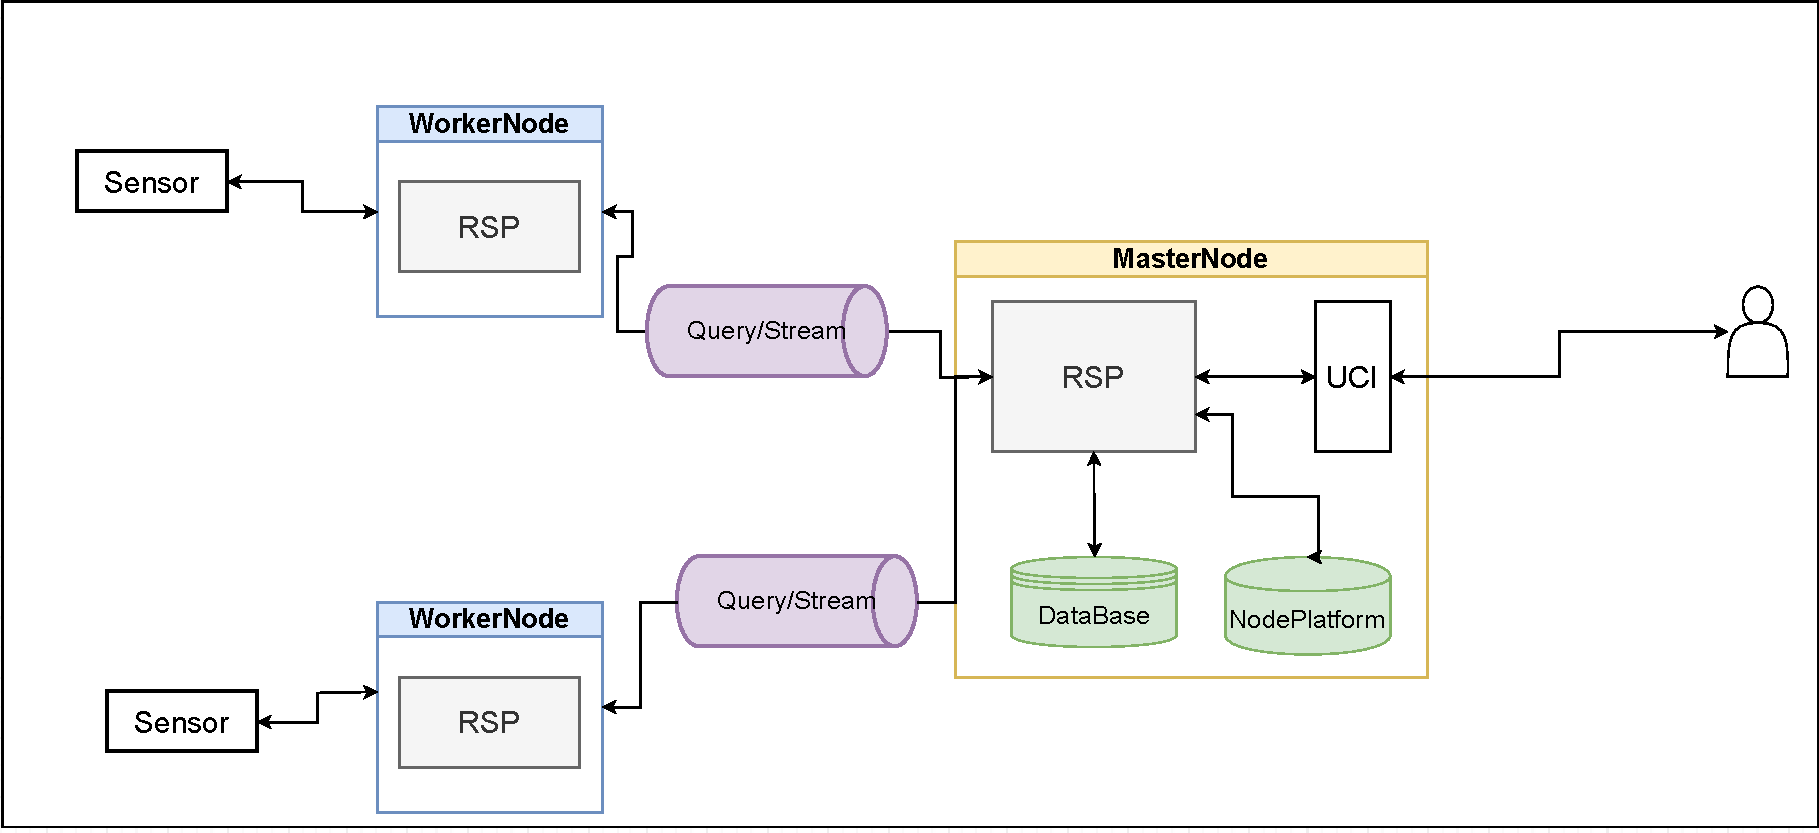
\includegraphics[width=0.5\textwidth]{EDgeLayer.drawio.pdf}
%   \caption{The Edge Layer}
%   \label{fig:edgelayer}
% \end{figure*}


% \begin{figure*}[ht]
%   \centering
%   \begin{minipage}{0.49\textwidth}
%       \centering
%       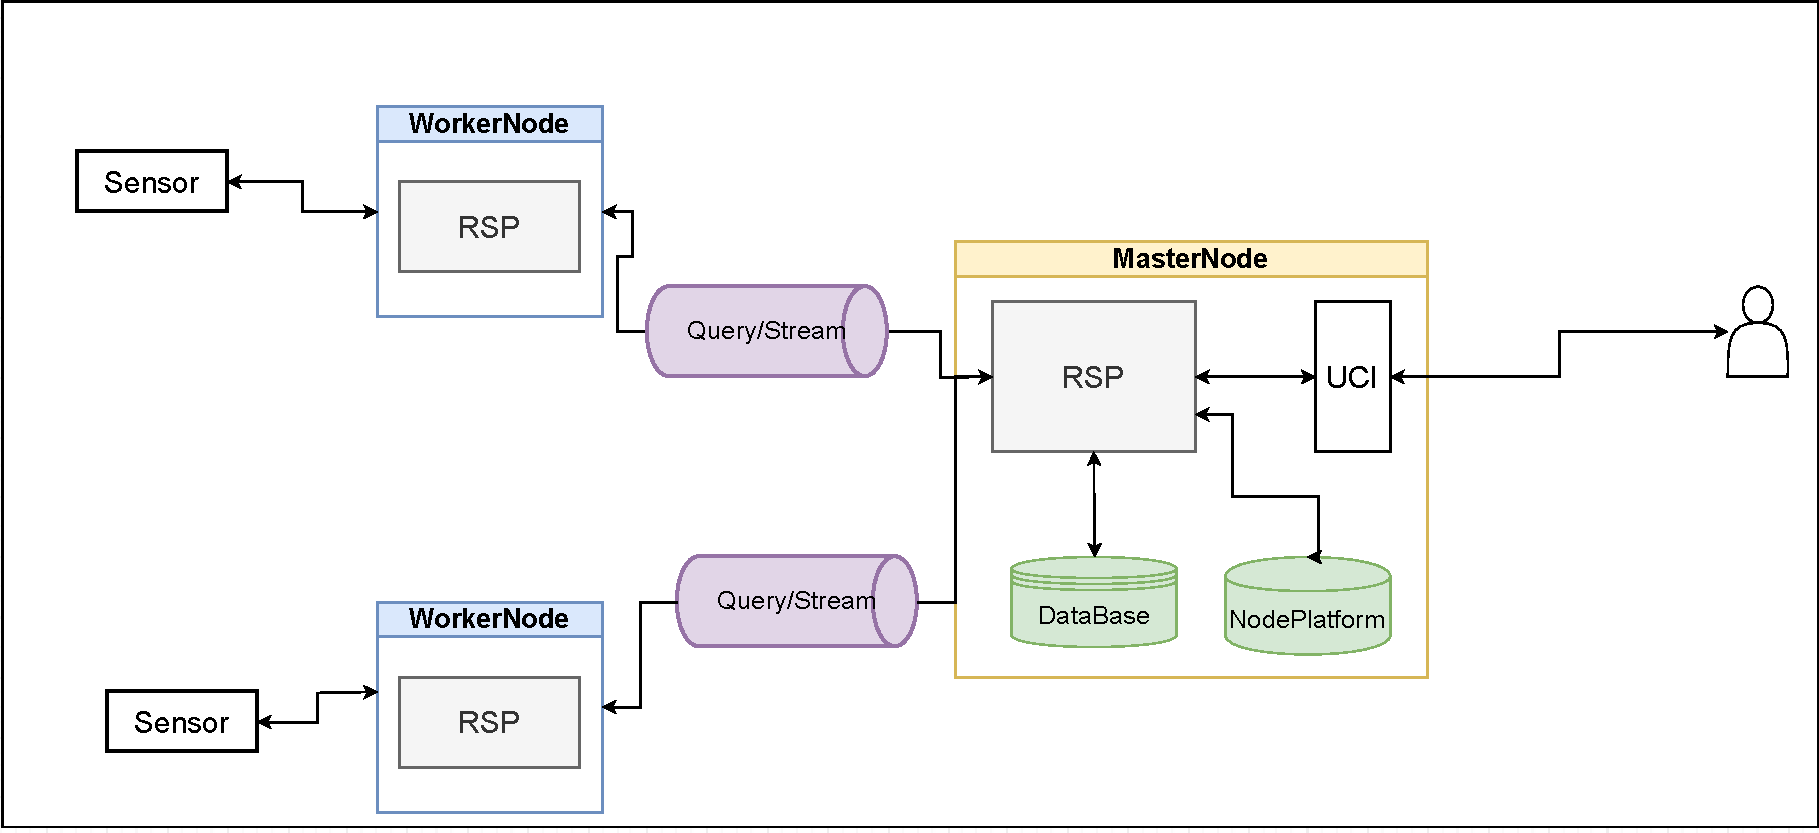
\includegraphics[width=\textwidth]{EDgeLayer.drawio.pdf}
%       \caption{The Edge Layer}
%       \label{fig:edgelayer}
%   \end{minipage}
%   \hfill
%   \begin{minipage}{0.49\textwidth}
%       \centering
%       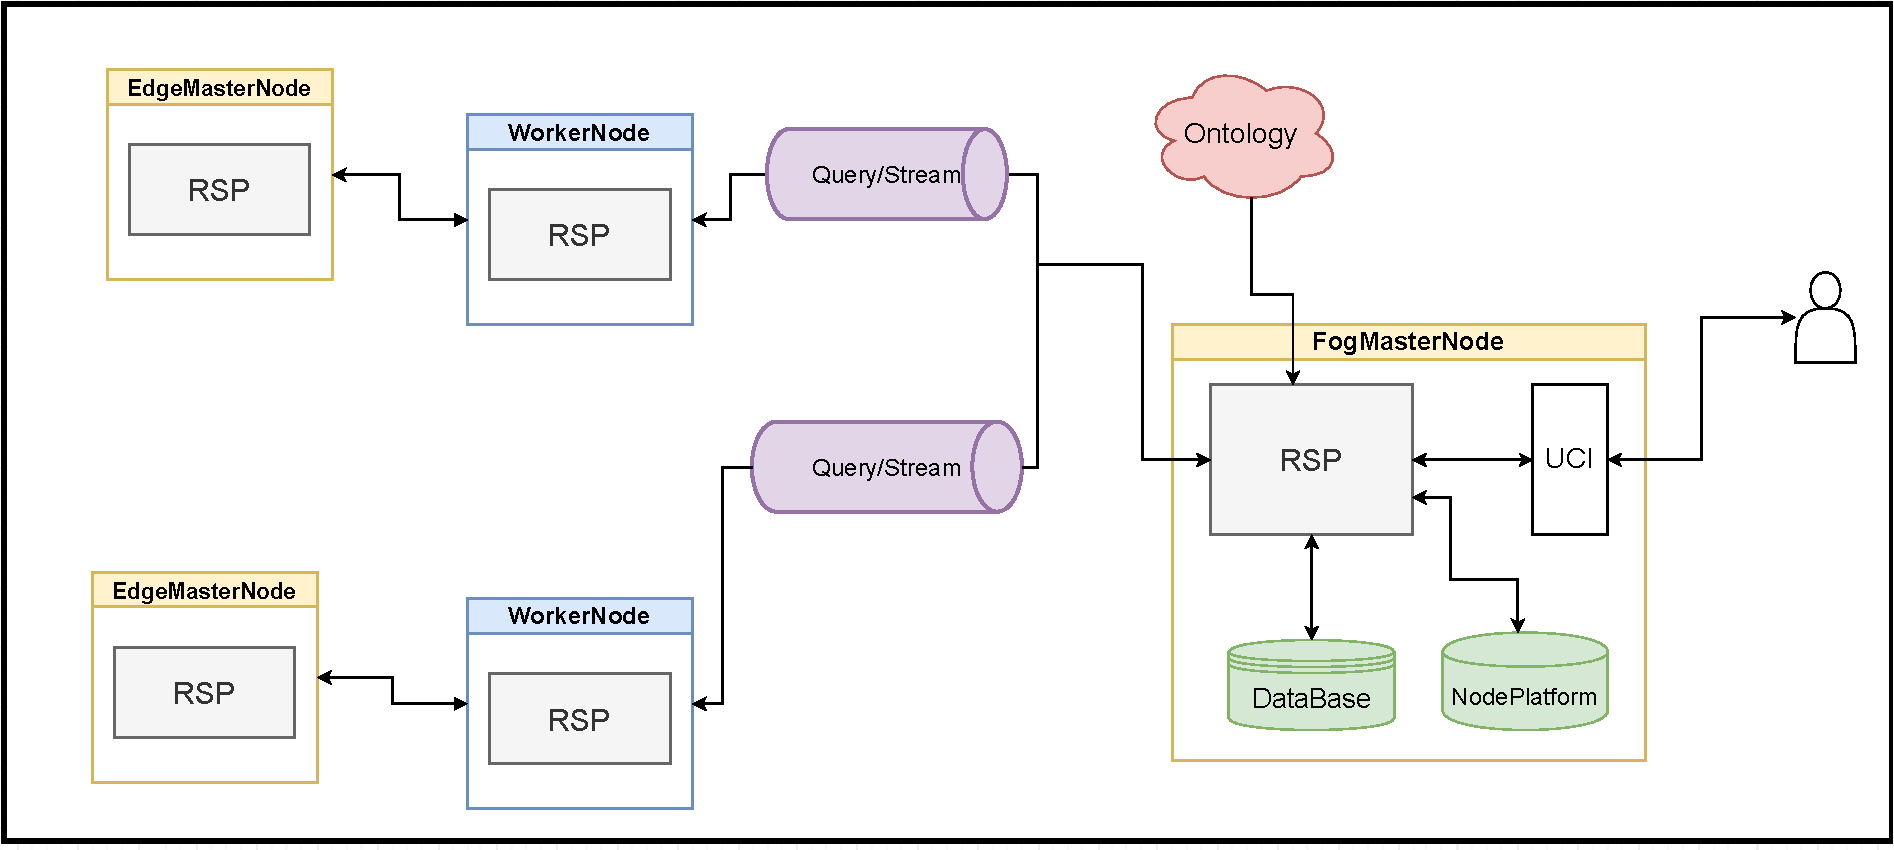
\includegraphics[width=\textwidth]{FogLayer.drawio.pdf}
%       \caption{The Fog Layer}
%       \label{fig:foglayer}
%   \end{minipage}
% \end{figure*}


\begin{figure}[t]
  \centering
  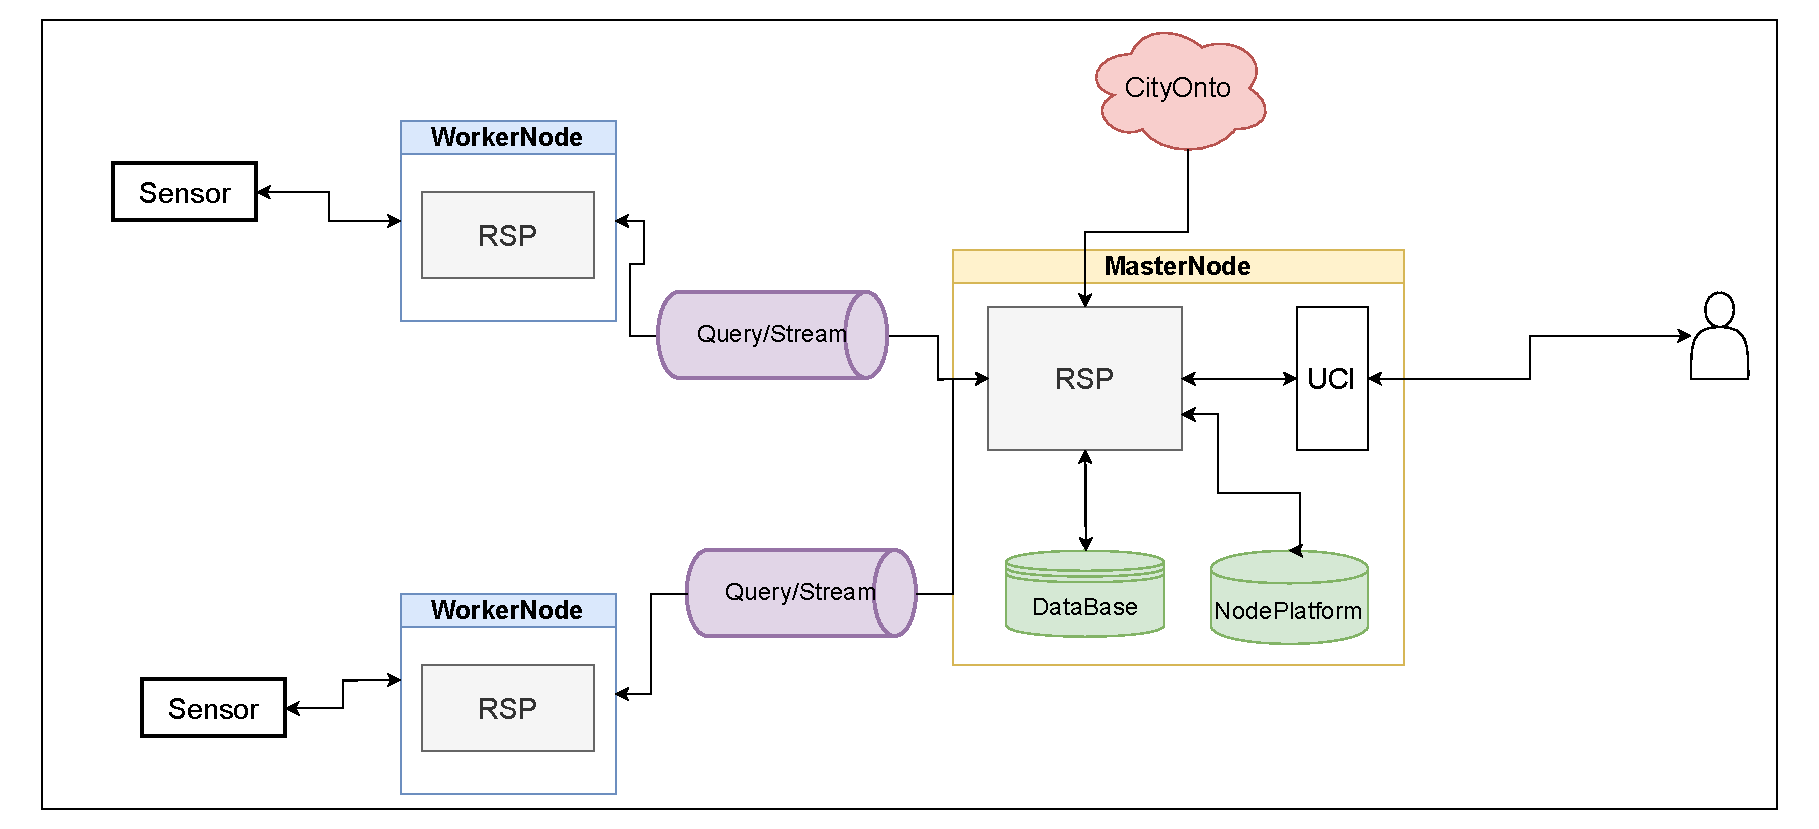
\includegraphics[width=\columnwidth]{EdgeLayer_New.drawio.pdf}
  \caption{The Edge Layer}
  \label{fig:edgelayer}
\end{figure}

\begin{figure}[t]
  \centering
  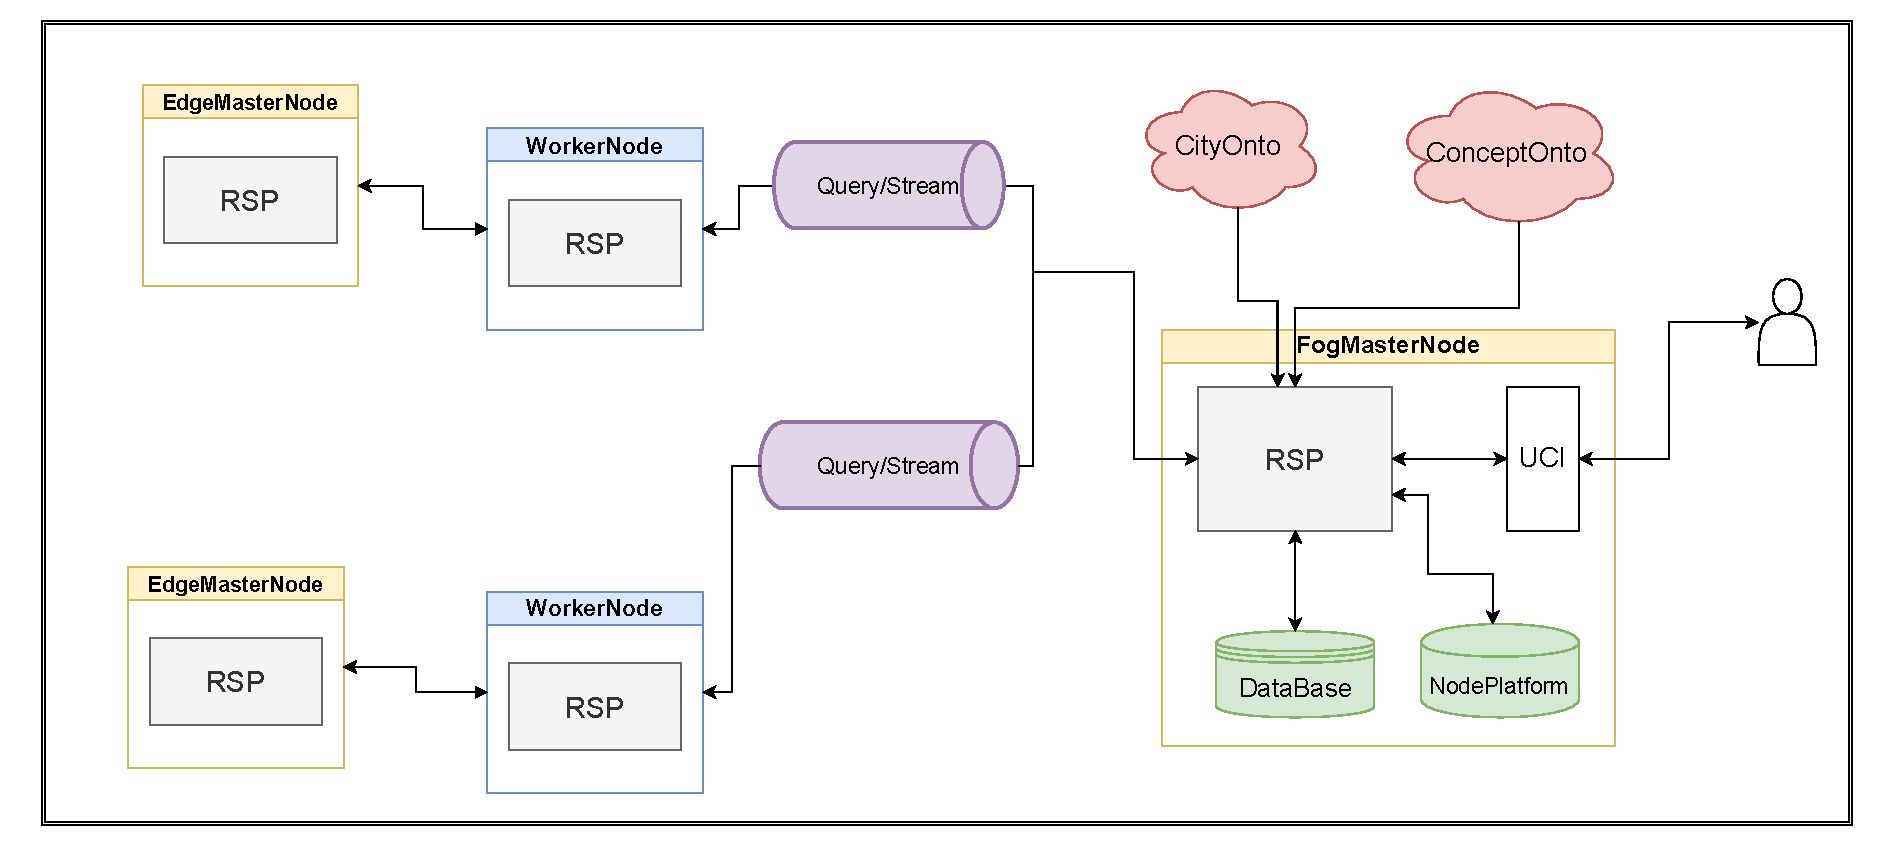
\includegraphics[width=\columnwidth]{FogLayer_New.drawio.pdf}
  \caption{The Fog Layer}
  \label{fig:foglayer}
\end{figure}


\begin{figure}[t] % Use [t] to attempt to place the figure at the top of the page
  \centering
  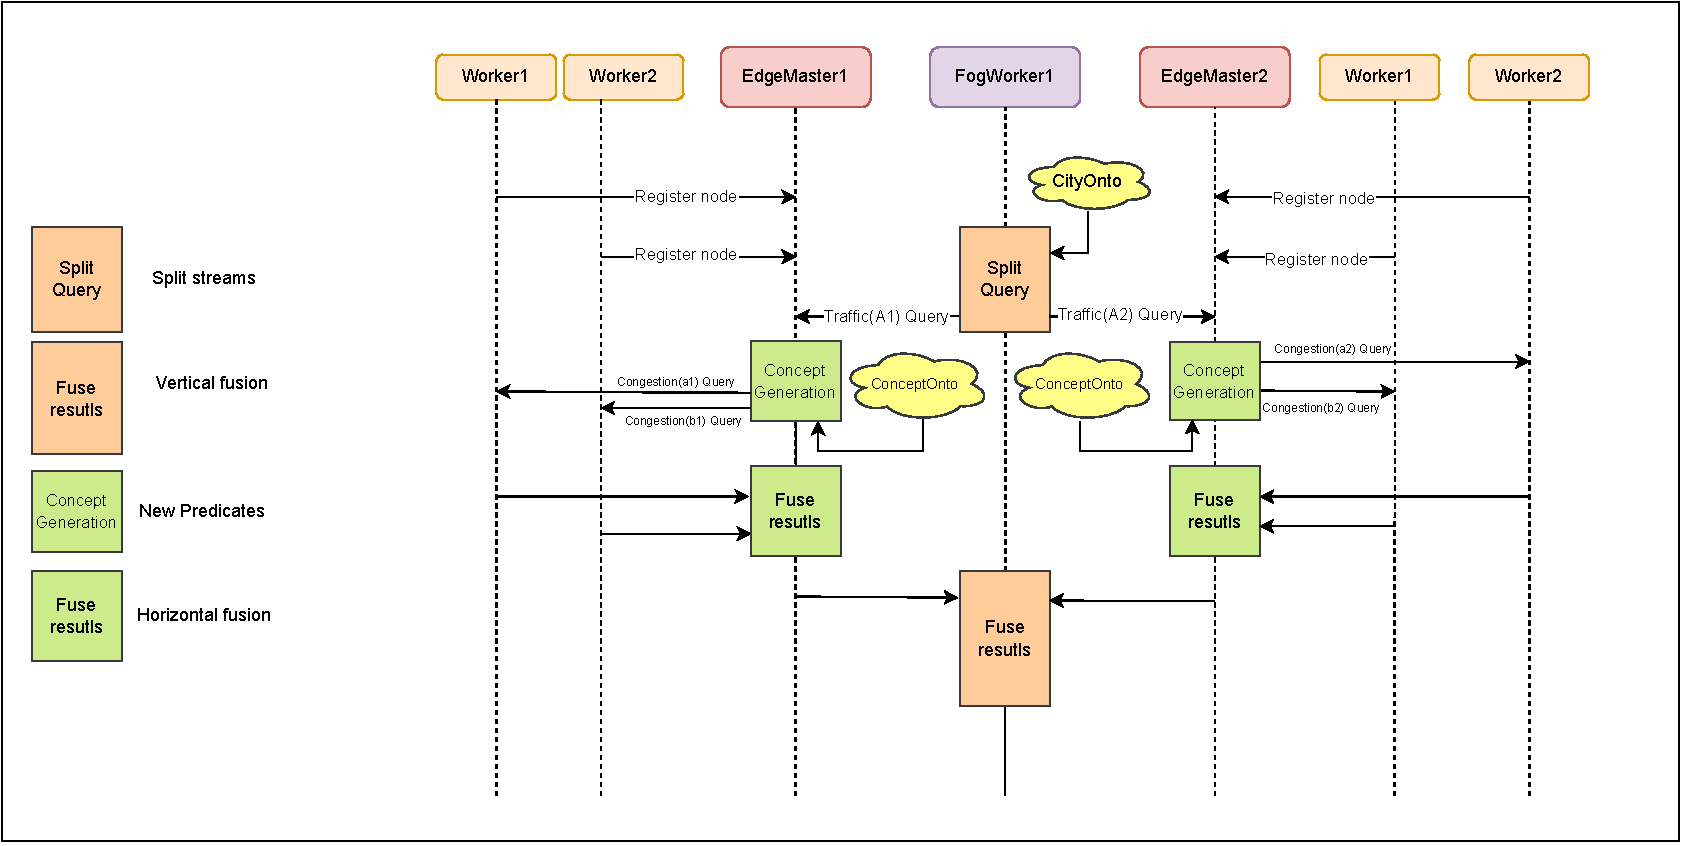
\includegraphics[width=\columnwidth]{Communication_new.drawio.pdf}
  \caption{Query execution request flow}
  \label{fig:queryexe}
\end{figure}


% The DiSIF framework, as illustrated in Figure \ref{fig:JDLandFusionprespective}, can be analyzed from the following aspects:

% \begin{itemize}
%     \item \textbf{Data Level}

% The designed framework is structured to manage data across distinct layers, transitioning from the edge layer to the cloud layer. The nature of the data becomes increasingly abstract, and its contextual complexity rises. At the edge layer, the data primarily comprises sensor data (Level one). In the fog layer, the data transforms into processed data or information streams. Queries performed at the edge layer focus on sensor data and involve operations related to data fusion. As queries progress to higher levels, they address broader concepts, such as traffic patterns, utilizing nodes in the fog layer for information fusion.

%     \item \textbf{Independent/Dependent Queries} 

% Queries defined in the DiSIF framework can be categorized into independent and dependent queries.
% Independent queries are usually inter-layer queries that can be executed simultaneously across multiple nodes, 
% with their results combined afterward. These queries are assigned from worker nodes in the upper layer to master nodes in the lower layer.


% Dependent queries, on the other hand, are intra-layer queries that must be executed sequentially and consecutively. The results of one
%  query are considered as input for another query. These queries are executed between worker and master nodes within a layer.
    

% \begin{figure*}
%   \centering
%   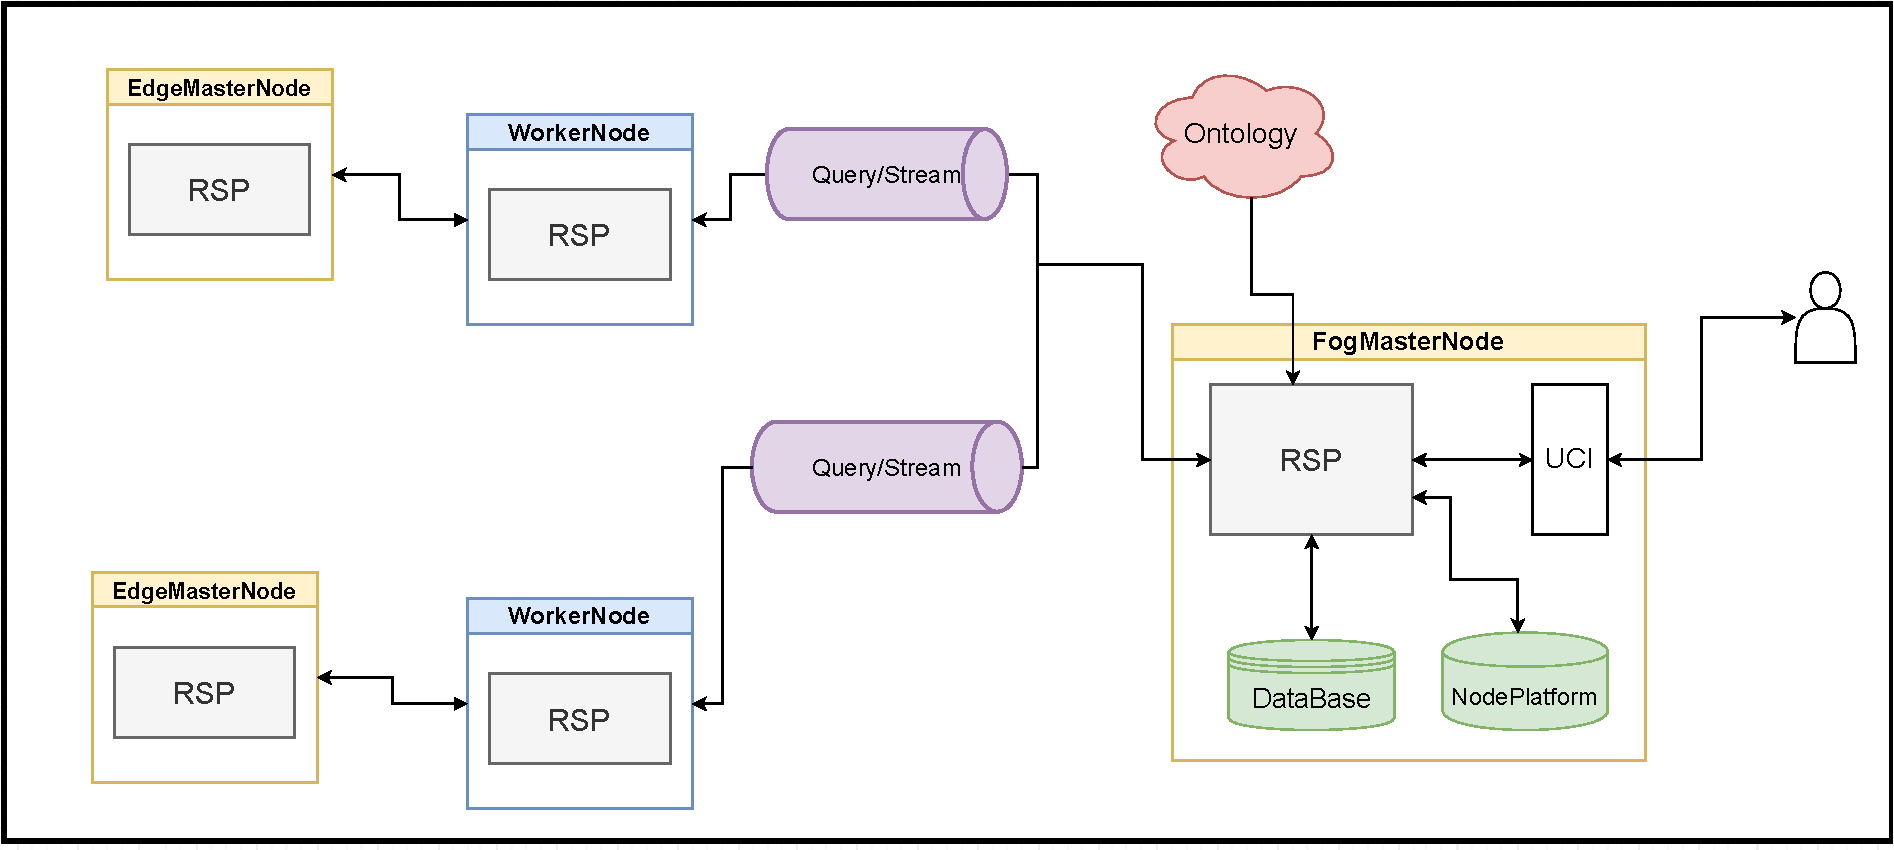
\includegraphics[width=0.5\textwidth]{FogLayer.drawio.pdf}
%   \caption{The Fog Layer}
%   \label{fig:foglayer}
% \end{figure*}


%     \item \textbf{Vertical vs. Horizontal Fusion} 


% Vertical fusion operations, resulting in an increase in the scale of the data.
%  In other words, the input and output of vertical fusion represent the same concept,
%   differing only in size and scale. For example, traffic data from multiple streets can be fused to generate traffic data for an entire area.



% Horizontal fusion, results in a change in the concept of the data. For instance, it involves fusing congestion data from a street to generate traffic data specific to that street. In this type of fusion, only the concept of the output data changes, while the scale and size of the data remain unchanged. Horizontal fusion can occur within each layer and between master and worker nodes.


    
%     \item \textbf{JDL Model Components}

%  In the DiSIF framework, the edge layer handles operations related to the JDL 
%  object refinement component, while situation refinement can be performed in the 
%  fog layer on the data received from the edge layer. Similarly, in the cloud layer, threat refinement operations can take place.
% \end{itemize}



% The subsequent section presents an overview of each layer in the DiSIF framework, aiming to deploy a Distributed Semantic JDL model.


% # node platform


\subsection{The DiSIF Framework: A Bridge Between the JDL Model and Digital Twin}

Akey innovation of the DiSIF framework is its structured
application of the Joint Directors of Laboratories (JDL) information fusion model within a three-layer distributed architecture
(edge, fog, and cloud). This approach underpins the creation
and maintenance of a comprehensive, real-time Digital Twin
in complex environments such as smart cities. As a dynamic
virtual representation of a physical system, a Digital Twin re
quires a continuous stream of processed data at various levels
of abstraction. The DiSIF framework systematically addresses
this requirement by aligning its architectural layers with the
functional levels of the JDL model.

\begin{itemize}
  \item Level 1: Object Refinement at the Edge.  The Edge Layer in the DiSIF architecture is responsible for
  initial, real-time processing tasks. It directly interfaces with
  sensors, transforming raw data streams into meaningful initial
  information. This process directly corresponds to JDL Level 1,
  Object Refinement. At this level, physical objects (e.g., vehicles, environmental sensors) are identified, and their basic attributes
  (e.g., location, speed, ID) are extracted and converted into a standard RDF format.
  
  Role in the Digital Twin: This layer forms the foundation
  of the Digital Twin. By processing data closest to the source,
  an initial, real-time digital representation of each object in the
  physical environment is created. This constitutes the birth of
  individual digital entities within the Digital Twin.

  \item Level 2: Situation Refinement in the Fog. The Fog Layer acts as an intermediate tier, receiving pro
  cessed information from edge nodes and fusing it to achieve a
   higher-level understanding of the overall situation. This function
   is equivalent to JDL Level 2, Situation Refinement. In this layer,
   using ontologies such as ConceptOnto, the relationships between
   different objects are analyzed to identify more complex events,
   such as "heavy traffic" or "congestion".
   Role in the Digital Twin: The fog layer enriches the Digital
   Twin by adding context awareness and an understanding of
   interactions. At this stage, the Digital Twin evolves from a
   collection of discrete objects into an integrated, intelligent virtual
   system capable of reflecting dynamic situations and the complex
   relationships between a smart city’s components.

   \item Level 3: Threat Refinement in the Cloud. The Cloud Layer, as the highest architectural tier, utilizes
   the enriched data from the fog layer for macro-level analysis,
   long-term prediction, and strategic decision-making. This level
   of processing aligns with JDL Level 3, Threat Refinement. By
   leveraging historical data and live information streams, this layer
   can forecast complex patterns and assess the potential impact of
   various scenarios.

   Role in the Digital Twin: This layer transforms the Digital Twin into a powerful simulation and forecasting tool. Here,
   the virtual model not only represents the present state but can
   also be used to test "what-if" scenarios and optimize city-wide management, moving from a reactive monitor to a proactive
   optimization engine.



\end{itemize}

\subsection{Horizontal and Vertical Fusion: Building a Comprehensive and Multi-Resolution Digital Twin}

The DiSIF framework leverages horizontal and vertical fusion to construct a comprehensive,
 multi-resolution Digital Twin of a City, effectively addressing the challenges 
 of heterogeneous and high-velocity IoT data streams. Horizontal fusion, implemented
  within each layer (edge, fog, and cloud) through a multi-agent system (MAS),
   decomposes complex queries into independent sub-queries for parallel execution,
    significantly enhancing processing speed and efficiency for tasks like object
     refinement, situation refinement, and threat refinement. Conversely, vertical
      fusion operates across the distributed JDL layers, utilizing the ConceptOnto
       ontology to transform high-level queries into lower-level concepts, ensuring
        semantic coherence and enabling hierarchical decision-making from localized,
         real-time insights at the edge to city-wide strategic analyses in the cloud. 
         This dual-fusion approach ensures scalability, privacy preservation,
          and timely analytics, making DiSIF a robust solution for operationalizing multi-scale Digital Twins.

\subsubsection{ Vertical Fusion: Enabling a Multi-Resolution Digital Twin}
The DiSIF framework employs vertical fusion to construct a multi-resolution Digital Twin of a City,
 enabling seamless hierarchical data integration across its distributed layers
  (edge, fog, and cloud) to support analytics at varying scales. Vertical fusion
   utilizes the ConceptOnto ontology to transform high-level analytical
    queries into lower-level concepts, ensuring semantic coherence as data
     progresses from real-time, localized processing at the edge to comprehensive,
      city-wide insights in the cloud. For example, at the edge layer, 
      raw sensor data (e.g., vehicle speed from traffic sensors) undergoes object
       refinement to detect individual events. These results are propagated 
       to the fog layer, where situation refinement integrates them into broader
        patterns, such as identifying traffic congestion zones. In the cloud,
         threat refinement leverages these insights for strategic decisions,
          like optimizing city-wide traffic policies. By serially transforming
           concepts across the JDL-based layers, vertical fusion ensures
            that the Digital Twin captures multi-resolution insights—from granular,
             real-time vehicle detection to long-term urban planning—while
              maintaining scalability and privacy for high-velocity IoT data streams.

\subsubsection{Horizontal Fusion:Enabling Scalable Parallel Analytics in Digital Twins}

The DiSIF framework leverages horizontal fusion to enhance scalable 
parallel analytics within a Digital Twin of a City by enabling concurrent
 query execution within each layer (edge, fog, and cloud) through a multi-agent system (MAS).
  Horizontal fusion decomposes complex queries into independent sub-queries,
   which are distributed across agents within a layer for parallel processing, 
   with results aggregated by a master agent to ensure efficient and scalable analytics.
    For example, at the edge layer, horizontal fusion processes high-velocity
    IoT data streams, such as real-time vehicle detection from multiple traffic sensors,
     by parallelizing object refinement tasks across agents to minimize latency.
      In the fog layer, it supports situation refinement by concurrently analyzing semantic
       queries, such as identifying traffic congestion patterns across different city zones.
        Similarly, in the cloud layer, horizontal fusion enables parallel execution
         of threat refinement tasks, like anomaly detection in city-wide traffic data.
          By utilizing MAS for intra-layer parallel processing, horizontal
           fusion ensures rapid, resource-efficient handling of heterogeneous data, 
           contributing to the scalable and responsive analytics of the Digital Twin
            while maintaining low latency and high throughput.








\subsection{Edge Layer}

An overall view of the DiSIF framework’s Edge layer is
depicted in Figure \ref{fig:edgelayer}.
At the Edge layer, data processing and horizontal fusion operations are
performed directly on sensor data streams, providing the first
line of real-time analysis in the Digital Twin of the City. Worker
agents at this layer are responsible for receiving raw data from
sensors, executing assigned queries from the master node, and
transmitting processed result streams back to the master agent.
Master agents at the edge layer manage user queries received via
the User Communication Interface (UCI), store data in the local
database, and maintain a registry of worker agents through the
AgentPlatform. They orchestrate query execution by assigning
sub-queries to worker agents based on cityOnto, aggregating results, and ensuring
efficient data flow upwards to the fog layer.




\section*{AgentPlatform}



\begin{table}[t]
  % \centering

  \captionsetup{justification=raggedright, singlelinecheck=false} % Left-align the caption
  \caption{\newline Example of NodePlatform}
  \vspace{-1em} % Adjust this value to remove blank space if necessary


  % \captionsetup{justification=raggedright} % Left-align the caption
  % \caption{Example of NodePlatform} % Move caption above the tabular
  \begin{tabular}{cccc}
  \hline
  \textbf{Node} & \textbf{Concept} & \textbf{Location} & \textbf{Master} \\
  \hline
  $N^w_1$ & $Congestion$ & $loc1$ & $N^m_1$ \\
  $N^w_1$ & $Congestion$ & $loc2$ & $N^m_1$ \\
  $N^w_2$ & $Traffic$    & $loc3$ & $N^m_3$ \\
  $N^w_3$ & $Congestion$ & $loc5$ & $N^m_2$ \\
  \hline
  \end{tabular}
  \label{tab:NodePlatformTbl}
  \end{table}


  % #=================


  % #===========
  The AgentPlatform, as outlined in Table \ref{tab:NodePlatformTbl},
   manages the registration and coordination of worker agents and their 
   corresponding master agents within each layer of the DiSIF framework.
    It maintains critical metadata, such as agent identifiers, to support 
    dynamic and flexible operations. Unlike traditional systems where agents
     are tied to specific locations, each agent in DiSIF can perform a variety
      of functions and process data from any location as needed. The platform enables
       the decomposition of complex queries into sub-queries, which are dispatched to
        worker agents capable of analyzing data streams from diverse sources,
         regardless of geographic constraints. The master agent's database component
          aggregates incoming data streams from worker agents, facilitating
           efficient query execution. The User Communication Interface (UCI) serves
            as the centralized gateway for user interactions, receiving 
            queries and delivering results, ensuring seamless communication across the system.





% \begin{algorithm*}
% \caption{RegisterWorkerNode}\label{register_worker_node}
% \begin{algorithmic}[1]
%     \Procedure{RegisterWorkerNode}{\textit{workerNode}}
%     \State\textit{WorkerNode} publish \textit{joinRequest} message with metadata to Kafka
%     \State Receive \textit{joinRequest} message at \textit{masterNode}
%     \State \textit{masterNode} store \textit{workerNode}'s metadata in \textit{Nodeplatform}
%     \State \textit{masterNode} send \textit{joinResponse} message to \textit{workerNode} with \textit{masterNode} information
%     \State Receive \textit{joinResponse} at \textit{workerNode} and store \textit{masterNode}'s information
%     \EndProcedure
% \end{algorithmic}
% \end{algorithm*}


At the Edge layer, vertical fusion operations—aligned
 with the object refinement phase of the semantic JDLmodel—are
 performed on incoming data. Specifically, the Edge layer col
lects and preprocesses raw data from physical city components,
 such as traffic lights, smart waste bins, or weather sensors em
bedded in specific buildings. This preprocessing, conducted
 at the object refinement level, transforms raw sensor data into
 structured semantic representations (e.g., RDF triples) to enable
 real-time updates of individual object states within the Digital
 Twin, such as the status of a specific vehicle or the temperature at
 a particular urban location. These fused and processed streams
 are then forwarded to worker agents in the Fog layer for higher
level fusion and decision-making.



%\section*{Metadata Information:}

%\begin{itemize}
%    \item URL address related to \textit{workerNode}.
%    \item Resources of \textit{workerNode}.
%    \item Set of conceptual predicates that the workerNode can generate (\textit{predicate}s of \textit{workerNode}).
%    \item \textit{streamIRI} (identifiers of streams that \textit{workerNode} can inspect and process).
%\end{itemize}

\subsection{Fog layer}

An overall view of the DiSIF framework’s Fog layer is illus
trated in Figure  \ref{fig:foglayer}. Within the Fog layer, data is processed and
 fused at the level of concept streams rather than raw data streams,
 reflecting a higher level of semantic abstraction essential for the
 Digital Twin of a City. Similar to the Edge layer, worker nodes
 in the Fog layer receive these concept streams from the Edge
 layer and execute queries assigned by their master nodes.
 Master nodes at the Fog layer handle multiple responsibili
ties: receiving user queries via the User Communication Inter
face (UCI), storing and managing data in the local database, reg
istering and retrieving information about worker nodes through
 the NodePlatform, assigning queries to worker nodes, receiving
 processed data streams, and performing fusion operations on the
 aggregated streams.
 The component architecture of the Fog layer closely mirrors
 that of the Edge layer but operates on semantically richer data.
 CityOnto ontology enables the Fog layer to integrate and interpret diverse urban data
 streams, supporting situation refinement and contextual decision
making. Within the master node, vertical fusion completes the
 situation refinement phase by combining heterogeneous concept
 streams to generate comprehensive, higher-level urban insights.


 Query Processing in the Fog Layer

 Algorithm 4 details the query response process within the
 master node of the Fog layer. The master node handles two
 primary query types: 
 SPARQL queries (line 4), which address
  static queries based on stored database information, and C-SPARQL queries (line 6), which manage continuous queries
facilitates data-driven decision-making for strategic urban man
over streaming data, essential for real-time Digital Twin opera
tions. At line 7, the algorithm checks if the semantic concepts
referenced in the query have been registered by any agent within
the AgentPlatform. The master node then aggregates the results from these
distributed executions (lines 9 to 11).
Algorithm 2 further elab
orates on query execution: if the node corresponding to the
concept and location extracted from the user’s query is found,
data retrieval, query execution, and result return are performed
(lines 6 to 8). If no matching node is found (line 10), the system
selects an alternative node from those previously registered in
the NodePlatform for the relevant master node and requested
location/stream. Subsequently, lines 11 and 12 utilize the Con
ceptOnto ontology to extract all necessary elements to construct
a query capable of generating the new semantic concept. Line
13 executes query construction via Algorithm 3. Finally, line 14
updates the NodePlatform to include the new concept for the se
lected node and location, and line 15 dispatches the constructed
query to the selected node for execution.

The Fog layer aggregates and integrates processed data from
the Edge layer to perform situation refinement, a critical step
in generating higher-level insights for the Digital Twin. This
involves combining concept streams to identify complex urban
patterns, such as traffic flow trends across a district, energy con
sumption profiles of a building block, or air quality variations
in a neighborhood. By leveraging the cityOnto ontology for
vertical fusion and horizontal fusion for situation refinement, the
Fog layer produces semantically enriched insights that enhance
contextual decision-making. These fused streams are then for
warded to the Cloud layer for city-wide analysis and strategic
decision-making.











\subsection{Cloud layer}

In the Cloud layer of the DiSIF framework, semantic fusion
operations are performed on the aggregated concept streams re
ceived from the Fog layer, enabling threat refinement at a macro,
city-wide level within the Digital Twin of a City. This layer
acts as the central hub where global concept streams are stored
in a comprehensive database, supporting long-term analysis
and predictive modeling essential for strategic urban manage
ment. Heavy computational tasks, such as traffic prediction and
anomaly detection, are executed periodically or on-demand us
ing both historical data and continuous streams from the Fog
layer. Traffic prediction, for example, forecasts congestion and
f
low patterns across various city locations, providing critical
insights for proactive traffic management and urban planning
within the Digital Twin environment.


\subsection{Query Management: Ensuring the Real-Time Viability of the Digital Twin}

The DiSIF framework ensures real-time synchronization of a Digital Twin of a 
City by efficiently processing high-velocity IoT data streams through an
 optimized query execution model. Using a multi-agent system (MAS), complex 
 queries are broken into sub-queries for parallel execution within each layer
  (edge, fog, cloud) via horizontal fusion, e.g., concurrent vehicle detection
   at the edge. Master agents aggregate results, while vertical fusion, using ConceptOnto,
    transforms high-level queries across layers for coherent analytics, like traffic
     flow optimization. This MAS-driven approach ensures low-latency, scalable query
      processing, maintaining the Digital Twin's real-time viability.

\subsubsection{ Parallel Execution of Independent Queries for Rapid Up dates}

Many update operations within a Digital Twin, such as fetch
ing the instantaneous status of thousands of distributed sensors
 or assets across a city, are inherently independent of one another.
 The DiSIF framework has the capability to break down an inde
pendent query into multiple sub-queries and execute each one in
 a parallel and efficient manner across different agents (Worker
 agents). Experimental results demonstrate that this distributed
 approach significantly optimizes query execution time.
 This parallel execution translates to a substantial reduction
 in the time required to aggregate data and refresh the overall
 state of the Digital Twin. Consequently, the latency between
 an event occurring in the physical world and its reflection in
 the virtual model is minimized, which underpins the "real-time"
 nature of the Digital Twin.


 \subsubsection{ Efficient Handling of Dependent Queries for Complex Simulations}

 Complex simulations and deep analytics in a Digital Twin of a City often
  involve dependent queries, where the output of one query serves as the input
   for the next, essential for modeling multifaceted urban phenomena (e.g., analyzing
    the impact of traffic congestion on air pollution). The DiSIF framework leverages
     the JDL fusion model to manage these complex situations effectively.
      By distributing dependent queries across its three-layer architecture
       (edge, fog, and cloud), DiSIF employs a multi-agent system (MAS) within
        each layer to execute sub-queries in parallel via horizontal fusion,
         while vertical fusion, supported by the ConceptOnto ontology, ensures
          seamless concept transformation across layers. Unlike centralized 
          approaches, where sequential processing on a single agent causes linear
           increases in response time, DiSIF’s distributed JDL model eliminates
            this bottleneck, significantly reducing total execution time. 
            This capability enables the Digital Twin to perform multi-step
             simulations in real-time, maintaining synchronization with the
              physical world and delivering timely, actionable insights for urban decision-makers.


\subsubsection{ Support for Dynamic and Complex Queries for an Adaptive Digital Twins}

For a Digital Twin to be an effective management and an
alytical tool, it cannot be limited to executing only predefined
queries. The urban environment is dynamic and unpredictable,
 constantly presenting new scenarios and unforeseen analytical
 needs. The DiSIF framework addresses this critical requirement
 by supporting
 complex and dependent queries that are not predefined and
 can be introduced at runtime.
 Unlike many systems that focus on executing predefined
 tasks or queries, a complex query can be introduced into the
 DiSIF architecture at any moment by a user or another service.
 These types of queries require the results of other queries that
 have been previously executed in the system to run. The DiSIF
 architecture manages this process optimally.

 \begin{itemize}
  \item  Dynamic Execution within Layers: The execution of these
  new, complex queries is handled by the Master Nodes in each
  layer, while their prerequisites (pre-queries) are executed by the
  Worker agents of the same layer.

  \item Automatic Query Construction: 
  When a new query requires a concept not yet defined in the system,
   the DiSIF framework utilizes the ConceptOnto ontology within its JDL-based architecture
    to automatically extract relevant elements and construct a new query.
     By leveraging ConceptOnto, DiSIF maps high-level concepts to lower-level
      data representations across the JDL layers (edge, fog, and cloud),
       enabling seamless query generation. This process ensures that complex,
        undefined concepts are dynamically resolved through vertical fusion,
         maintaining semantic coherence and supporting real-time analytics for the 
         Digital Twin of a City.


  This capability provides the Digital Twin with a high degree
  of adaptability. For instance, when faced with an unforeseen
  crisis (such as an extreme weather event or a sudden public
  health issue), city managers can define and execute entirely new
  analytical queries to assess the cross-system impacts (e.g., the
  effect of rainfall on traffic and access to emergency services).
  DiSIF’s ability to dynamically process such queries ensures
  that the Digital Twin remains a living, evolving tool capable of
  responding to emergent urban challenges.

 \end{itemize}






 \begin{figure}[t] % Use [t] for top placement
  \centering
  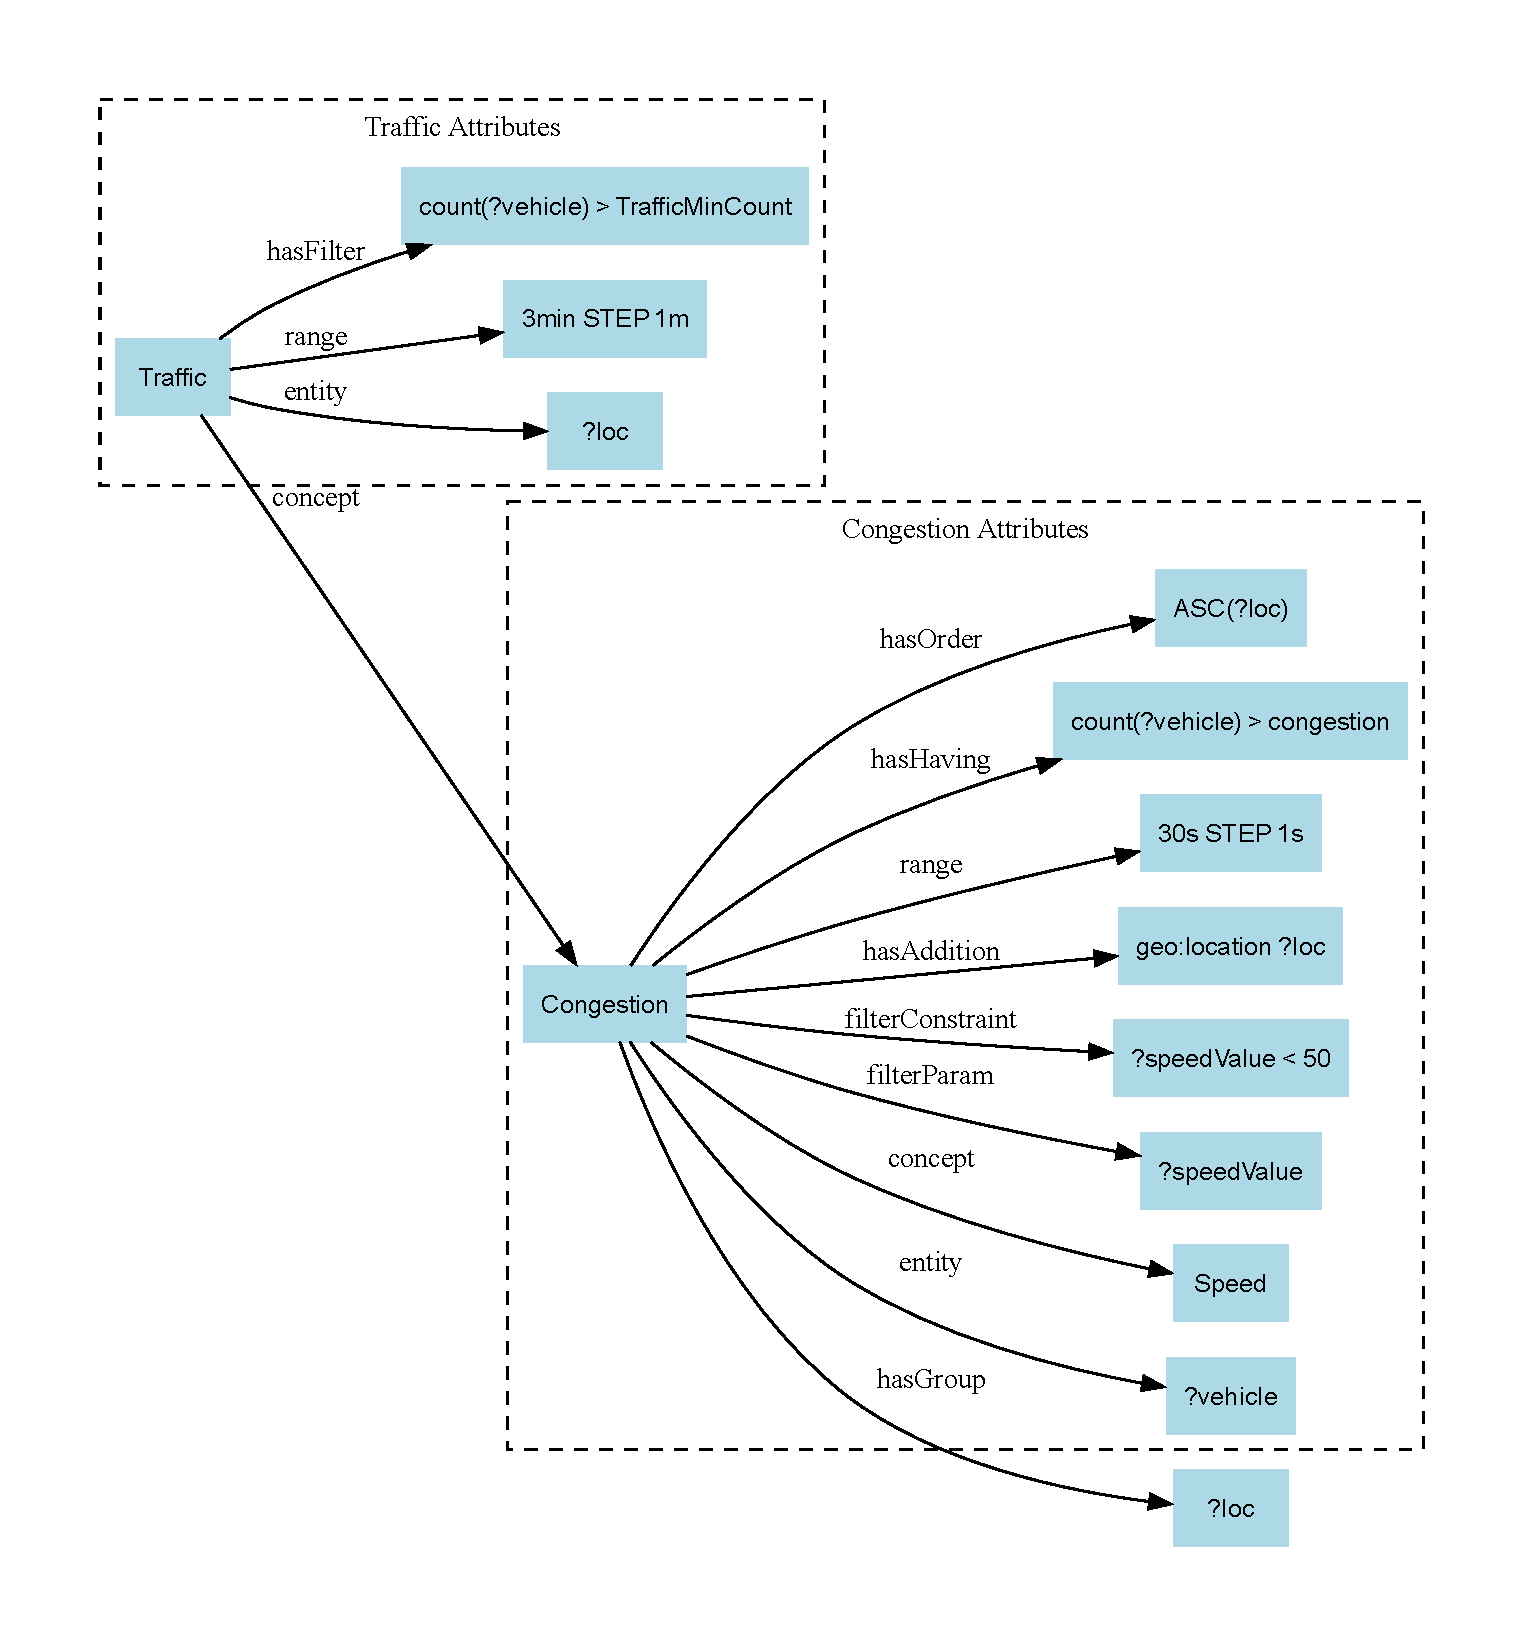
\includegraphics[width=\columnwidth]{ConceptOnto_GraphViz_new.pdf}
  \caption{Concept Ontology}
  \label{fig:conceptonto}
\end{figure}







\begin{figure}[t]
  \centering
  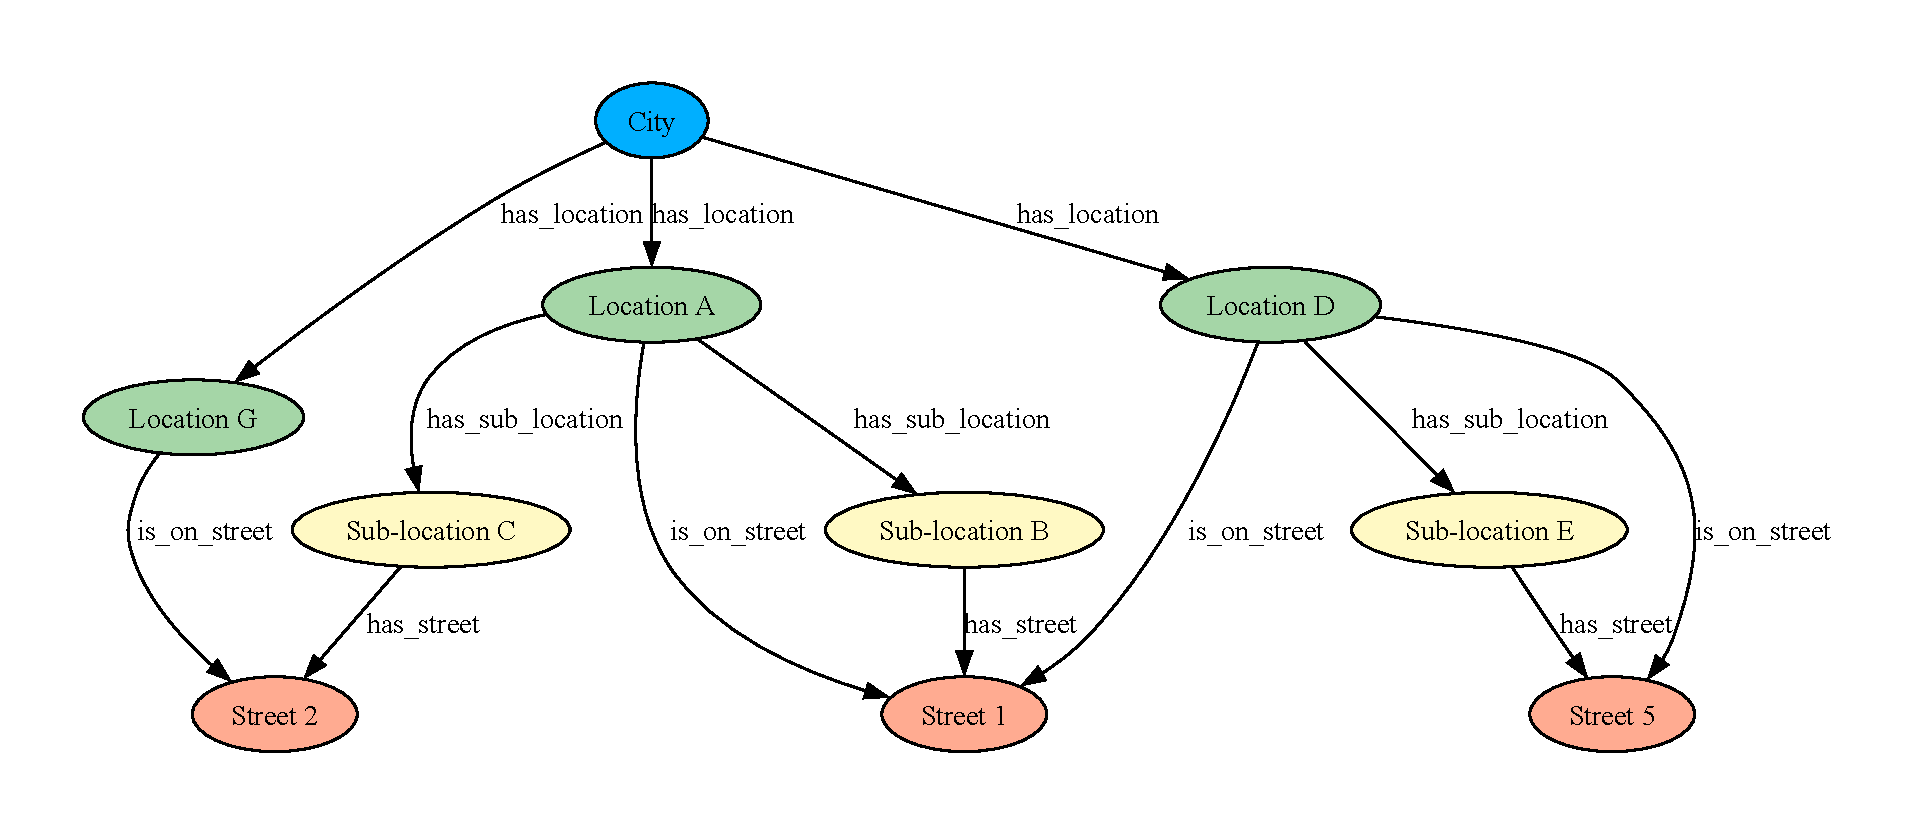
\includegraphics[width=0.5\textwidth]{cityOnto_graph.pdf}
  \caption{CityOnto example}
  \label{fig:CityOnto}
\end{figure}

\begin{figure}[t]
  \centering
  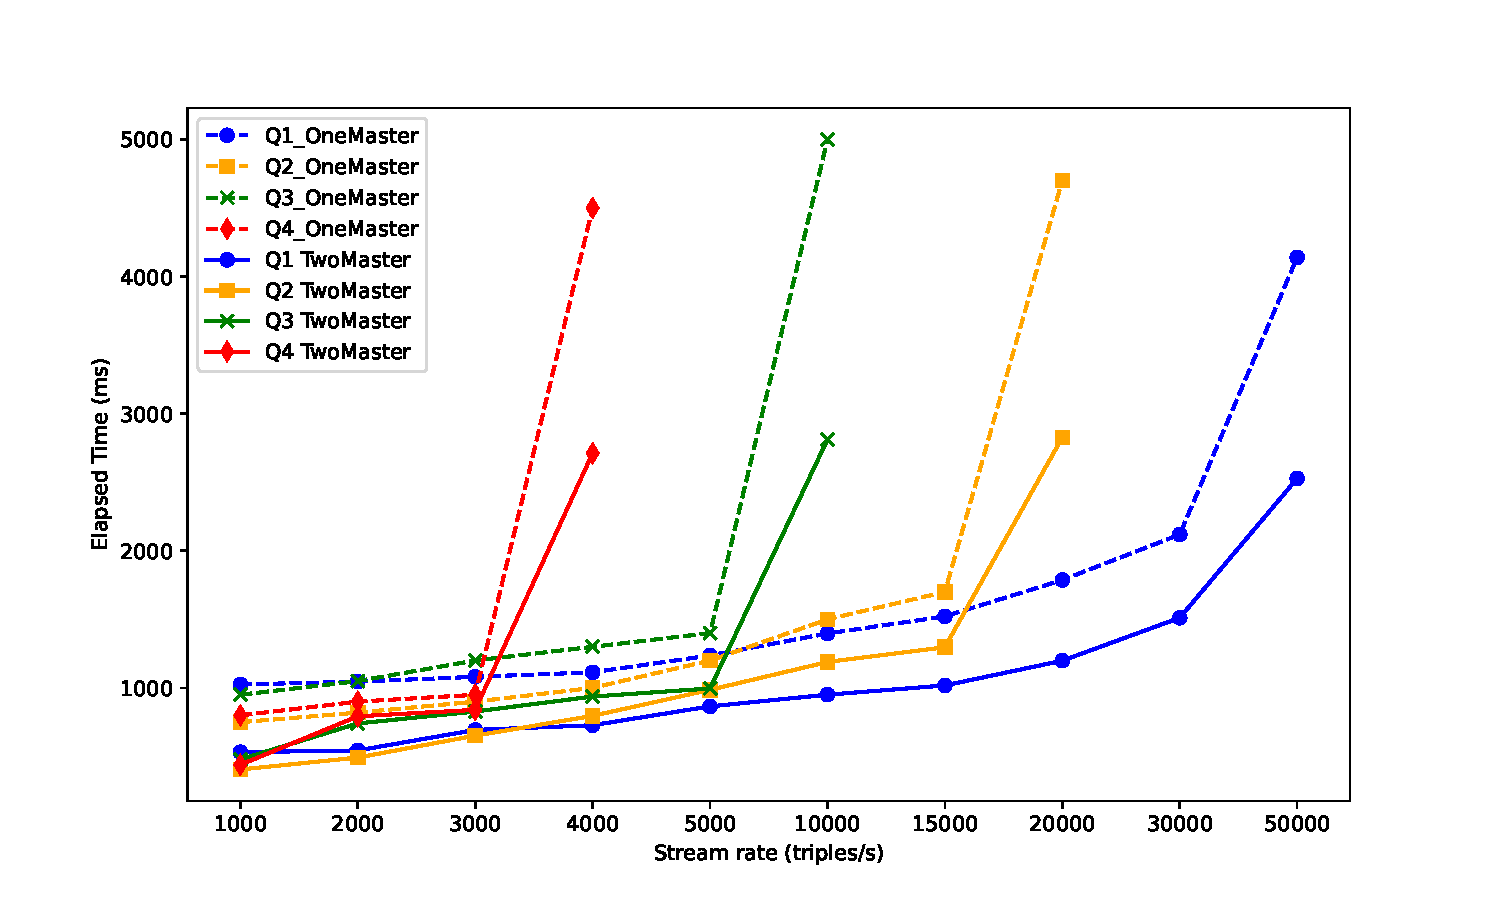
\includegraphics[width=\columnwidth]{result_TwoMaster_OneMaster.pdf}
  \caption{Object refinement performance: independent query execution time for different master nodes}
  \label{fig:resultTwoMasterOneMaster}
\end{figure}

\begin{algorithm}[t]
  \caption{Process Query}\label{alg:conceptQuery}
  \begin{algorithmic}[1]
  
  \Procedure{ProcessQuery}{$query$}
    \While {$True$}
        \State $Concepts, Locations \gets ExtractConceptsLocations(query)$
        \State $node \gets findNode(Concepts, Locations)$
  
        \If {$node$ exists}
            \State ListenOnNode($node$)
            \State $result \gets Execute(query)$
            \State \Return $result$
        \Else
            \State $node \gets SelectWorkerNode()$
            \State $Entity, Range, hasAddition, ConceptNew,$
            \Statex \hspace{1em} $filterParam, filterConstraints, hasGroup,$
            \Statex \hspace{1em} $hasHaving, hasOrder \gets$
            \Statex \hspace{1em} GetParameterFromConceptOnto(Concepts)
            \State $NewQuery \gets ConstructQuery(Concepts, Locations,$
            \Statex \hspace{1em} $Entity, Range, hasAddition, ConceptNew,$
            \Statex \hspace{1em} $filterParam, filterConstraints,$
            \Statex \hspace{1em} $hasGroup, hasHaving, hasOrder)$
  
            \State UpdateNodePlatform(Concepts, Locations, node)
            \State SendQueryToNode($NewQuery, node$)
        \EndIf
    \EndWhile
  \EndProcedure
  
  \end{algorithmic}
\end{algorithm}







\begin{algorithm}[t]
  \caption{Construct Query}\label{alg:constructquery}
  \begin{algorithmic}[1]
  \Procedure{ConstructQuery}{$Concept, Location, Entity, Range,$
  $hasAddition, ConceptNew, filterParam,$
  $filterConstraints, hasGroup, hasHaving, hasOrder$}
  
  \State $query \gets$
  \Statex \hspace{2em} \texttt{CONSTRUCT \{$?l$ concept:\{$Concept$\} $?a$\}} 
  \Statex \hspace{2em} \texttt{FROM STREAM \{$Location$\} [RANGE \{$Range$\}]}
  \Statex \hspace{2em} \texttt{WHERE \{ \{$Entity$\} concept:\{$ConceptNew$\} \{$filterParam$\},}
  \Statex \hspace{2em} \texttt{\{$Entity$\} \{$hasAddition$\},}
  \Statex \hspace{4em} \texttt{FILTER (\{$filterConstraints$\})}
  \Statex \hspace{2em} \texttt{\}}
  \Statex \hspace{2em} \texttt{GROUP BY \{$hasGroup$\}}
  \Statex \hspace{2em} \texttt{HAVING \{$hasHaving$\}}
  \Statex \hspace{2em} \texttt{ORDER BY \{$hasOrder$\}}
  
  \EndProcedure
  \end{algorithmic}
  \end{algorithm}

%\twocolumn % Switch to one column
\section{Evaluation}

The DiSIF framework is implemented in the Java programming environment. The codes written for the semantic nodes are independent of the communication layer, allowing the use of various communication channels such as MQTT or WebSocket. The communication channel in the DiSIF framework is based on Apache Kafka. In the system implementation, we utilize C-SPARQL as the RDF stream processor (RSP). 
Next, we explore the evaluation of the centralized JDL approach and the distributed JDL approach.

As mentioned, in the centralized JDL fusion model, generating the desired outputs requires collecting all the necessary data in a central node, where queries and corresponding components are executed on these aggregated data to produce the outputs. In contrast, in the distributed JDL approach, there is no need to send all data to a central node. Instead, by distributing query processing, only the query execution results are sent to other nodes.



Comparison of centralized and distributed JDL approaches can be analyzed from five perspectives:

\begin{itemize}
    \item \textbf{Network Load} 


In the centralized approach, since all RDF data needs to be sent to the master node, the network load increases significantly, leading to a decrease in network efficiency. The volume of raw data sent over the network to the master node is much larger than the processed data. In terms of the amount of data transmitted and data transfer speed, the approach of sending processed data is preferable to sending raw data. This makes the distributed JDL approach more network-efficient than the centralized JDL approach.
    
    \item \textbf{Execution Time of Dependent Queries}


In the JDL model, the situation refinement component, requiring the use of outputs from the object refinement component, executes dependent queries for output generation.
As subqueries need to be executed first to provide the necessary input for dependent queries, the time to produce outputs for dependent queries increases. In the centralized approach, both subqueries and dependent queries are executed on a single node, while in the distributed JDL approach, subqueries are executed on worker nodes, and dependent queries are executed on the master node. Consequently, the execution time of dependent queries is reduced, making it more efficient compared to the centralized approach.
    
    \item \textbf{Execution Time of Independent Queries}


    In the JDL model, the object refinement component includes independent queries that operate on raw data and do not require the execution of other queries as prerequisites. In the distributed approach, these queries can be executed across different nodes, enhancing the execution time of independent queries compared to the centralized scenario.
    
    \item \textbf{Memory Consumption}


 In the centralized JDL model, the execution of independent and dependent queries on a single node can significantly impact their memory consumption. On the other hand, the distributed JDL approach has demonstrated better memory management compared to the centralized approach.
    
    \item \textbf{Data Security}


 One of the challenges of the centralized JDL method is that all data must be sent from other nodes to the master node, posing potential security issues. In many applications, data from nodes cannot be transferred to the master node due to security concerns and must be used locally. Therefore, the distributed JDL approach is introduced to overcome this challenge. In this approach, there is no need to send raw data from other nodes to the central node, and data processing can be performed locally on local data, with the results sent to the master node. Thus, the security issue related to data transfer is mitigated in this distributed approach.
\end{itemize}



In this section, we analyze the centralized and distributed JDL approaches in terms of executing various JDL components.
To evaluate the object refinement component in the edge layer and the situation refinement component in the fog layer, we analyze the executing of independent and dependent queries, respectively, in both centralized and distributed scenarios.


%\onecolumn % Switch to one column
\begin{algorithm}[t]
  \caption{Query Response in masterNode}
  \label{alg:QueryresponsemasterNode}
  \begin{algorithmic}[1]
      \setstretch{1} % Adjust the spacing factor as needed
      \State \textbf{Input:} User query 
      \State \textbf{Output:} Query response

      \State Receive user query by UCI and send to RSP component
      \If{SPARQL query}
          \State Execute query on database and get results.
      \ElsIf{C-SPARQL query}
          \If{Query's concepts exist in NodePlatform}
              \If{Query's locations exist in NodePlatform}
                  \State Split the query by locations into independent sub-queries.
                  \State Assign each sub-query to corresponding node registered in NodePlatform.
                  \State Aggregate results of sub-queries. 
              \Else
                  \State Expand each query stream/location with its 
                  sub-streams/sub-locations according to the cityOnto.
                  \State Repeat the steps from line 6.
              \EndIf
          \Else
              \State Create a new query for generating the desired concept 
              based on Algorithm \ref{alg:conceptQuery} using the conceptOntology.
          \EndIf
      \EndIf
  \end{algorithmic}
\end{algorithm}





\subsection{Object refinement performance in the Edge layer}


The data in this layer consists of sensor data (level one), and the queries processed at this level are classified as level one or independent queries. 
Consequently, the fusion operation occurs at the sensor level, referred to as sensor/data fusion. Subsequently, the performance of the DiSIF framework is analyzed in terms of the execution time of level one/independent queries in the edge layer.

\subsubsection{Centralized and Distributed approaches}
In these experiments, we analyze the time required to execute queries Q1, Q2, Q3, and Q4
 (shown in \ref{sec:AppendixQueries}) from the perspective of the stream rate.


%\begin{figure*}
%  \centering
%  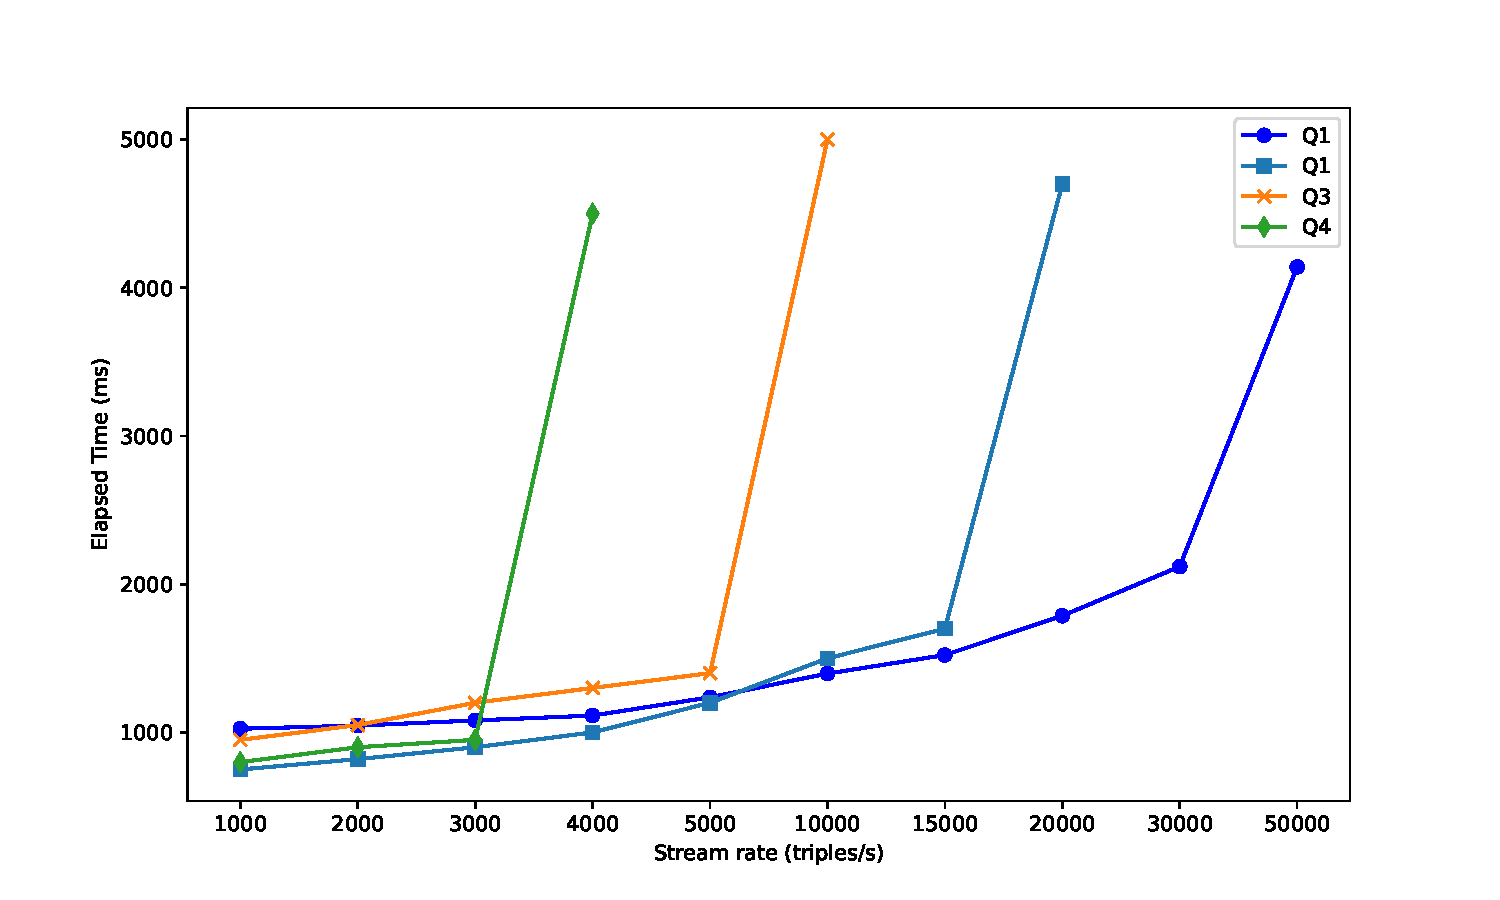
\includegraphics[width=0.8\textwidth]{C:/Users/Administrator/Desktop/Thesis_latex_Final/result_OneMaster.pdf}
%  \caption{Query execution time for different stream rates}
%  \label{fig:resultOneMaster}
%\end{figure*}


in Figure \ref{fig:resultTwoMasterOneMaster} , the results of executing various queries in the centralized scenario, where only one edge master node exists and for distributed approach with two edge master nodes,
 are presented. In this case, the execution time of queries is analyzed for different stream rates.
 As observed, for query Q1, the execution time experiences a sudden increase at a stream rate of 30000 triples/s.
 Similarly, query Q2 shows a sudden increase at a stream rate of 15000 triples/s, Q3 at 5000 triples/s, and finally, Q4 at 3000 triples/s. 

The reason for this phenomenon is that, in C-SPARQL, as the complexity of a query increases, its ability to manage high stream rates decreases.
 When the stream rate exceeds the response capacity of C-SPARQL, the execution time of the query experiences a sudden increase.
For this reason, in cases where a query is broken down into independent subqueries and multiple edge master nodes are available for query execution, 
each subquery can be executed on a separate edge master node and the results are then combined, enabling the main query to be executed in parallel. 
Consequently, the execution time of queries significantly improves in distributed approach.






As depicted in Figure \ref{fig:resultTwoMasterOneMaster}, the execution time for different stream rates is approximately halved. The reason for this slight increase in the execution time is that a short period is spent aggregating the results from these two nodes. Therefore, in comparison to the centralized approach for executing independent queries, this distributed scenario exhibits lower execution times.


\subsection{Situation refinement performance in the Fog layer}

In this section, we evaluate the performance of the distributed JDL fusion model in comparison to the centralized JDL, focusing specifically on the situation refinement component and the execution of dependent queries.
The scenarios of congestion detection and traffic discovery are examined as two dependent scenarios or queries.

The data flowing between nodes in the fog layer is categorized as level two. In other words, this data consists of processed information from the lower edge layer, rather than raw sensor data.  Consequently, the fusion operation at this level involves information fusion, and the queries executed by fog layer managers are focused on concepts that require prepared input data for their execution.

In the centralized JDL approach, obtaining the results of the situation refinement component requires the outputs of the object refinement component to be initially placed on the BUS associated with the centralized JDL. Consequently, object refinement and situation refinement queries are interdependent and must be executed in a sequential manner.


In the following, we evaluate the two components, object refinement and situation refinement, for the scenarios of congestion detection and traffic discovery, respectively.



\section*{Traffic Discovery Scenario}

For traffic discovery, the query \(Q_m\) is defined in \ref{sec:AppendixQueries} .

As indicated by query \(Q_m\), congestion event messages are received within 3-second windows. 
In this query, \texttt{?s} represents the streets (as locations) where congestion has occurred. If a street experiences congestion more than three times within a 3-second window, it is classified as congested. 
To execute this query, congestion event messages must be generated, which are produced by worker nodes within the same fog layer. 



\section*{Congestion Detection Scenario}

To evaluate the performance of both centralized and distributed JDL approaches for congestion detection,
 we employ various queries with diverse complexities as detailed in the \ref{sec:AppendixQueries} 
 as Queries \(Q_1\),\(Q_2\),\(Q_3\),\(Q_4\).

\textbf{Query \(Q_1\)}

In this query, the output highlights regions where the speed of at least one vehicle is below 50 km/h, indicating congestion. This query is specifically designed to detect congestion and generate congestion event messages based on the location, speed, and timestamp of vehicles within the specified stream.

\textbf{Query \(Q_2\)}

Continuing with the congestion detection scenario, Query \(Q_2\) identifies regions where at least three vehicles have speeds below 50 km/h, indicating congestion. The results are then sorted in ascending order based on location. This query establishes a more specific criterion for detecting congestion by taking into account both the speed condition and the minimum number of vehicles present in a given area.

\textbf{Query \(Q_3\)}

This query, similar to Query \(Q_2\), congestion is detected in areas with "2," "3," or "1" in their titles (?location). Additionally, the average speed of vehicles is returned as output for each location. This query offers insights into both congestion detection and the average speed of vehicles in specific locations.

\textbf{Query \(Q_4\)}

This operates similarly to Query \(Q_3\), with the difference that it uses UNION to also analyze areas whose title includes "4". This allows the query to provide insights into congestion detection and average speed in regions containing "2", "3", "1", or "4".


We evaluate the situation refinement component from three perspectives: query execution time, memory consumption,
 and network load. Each of these aspects will be examined in detail. Assume that executing the user query \(Q_m\) requires the execution of \(n\) prerequisite queries \(Q_i\).

\subsubsection{Query execution time}


In this section, we first express the formula for calculating the execution time of query $Q_m$ in centralized and distributed approaches as follows.


\begin{itemize}

\item Centralized approach


In the centralized approach, all raw data must be transferred from the worker nodes to the master node before executing query \( Q_m \) on the master node.

\begin{equation}
T_c = T_{\text{data transfer}} + \sum_{i \in N} T_{Q_i} + T_{Q_m}
\end{equation}

where \( T_{\text{data transfer}} \) is the time required to transfer raw data from all worker nodes to the master node, \( T_{Q_i} \) is the time taken to execute query \( Q_i \) on the master node, and \( T_{Q_m} \) is the time required to execute query \( Q_m \) on the master node.

\item Distributed approach

In the distributed approach, each query is executed on its respective worker node, and the results are transferred to the master node, where the query \( Q_m \) is executed. The execution time in the distributed approach is as follows:

\begin{equation}
T_d = \max(T_{Q_i}) + T_{\text{result transfer}} + T_{Q_m}
\end{equation}

As can be observed from the equations, in the centralized approach, the execution time increases linearly with the increase in the number of queries \( Q_i \). This is due to the sequential processing. In the distributed approach, the queries are processed in parallel, which reduces the execution time to the maximum time required to execute any of the \( Q_i \) queries. Therefore, for a large number of requests \( N \), the distributed approach significantly reduces the execution time compared to the centralized approach due to parallel execution.


% \begin{figure}[htb] % Inline figure with appropriate size
%   \centering
%   \begin{subfigure}{0.48\textwidth} % Use column width for inline placement
%     \centering
%     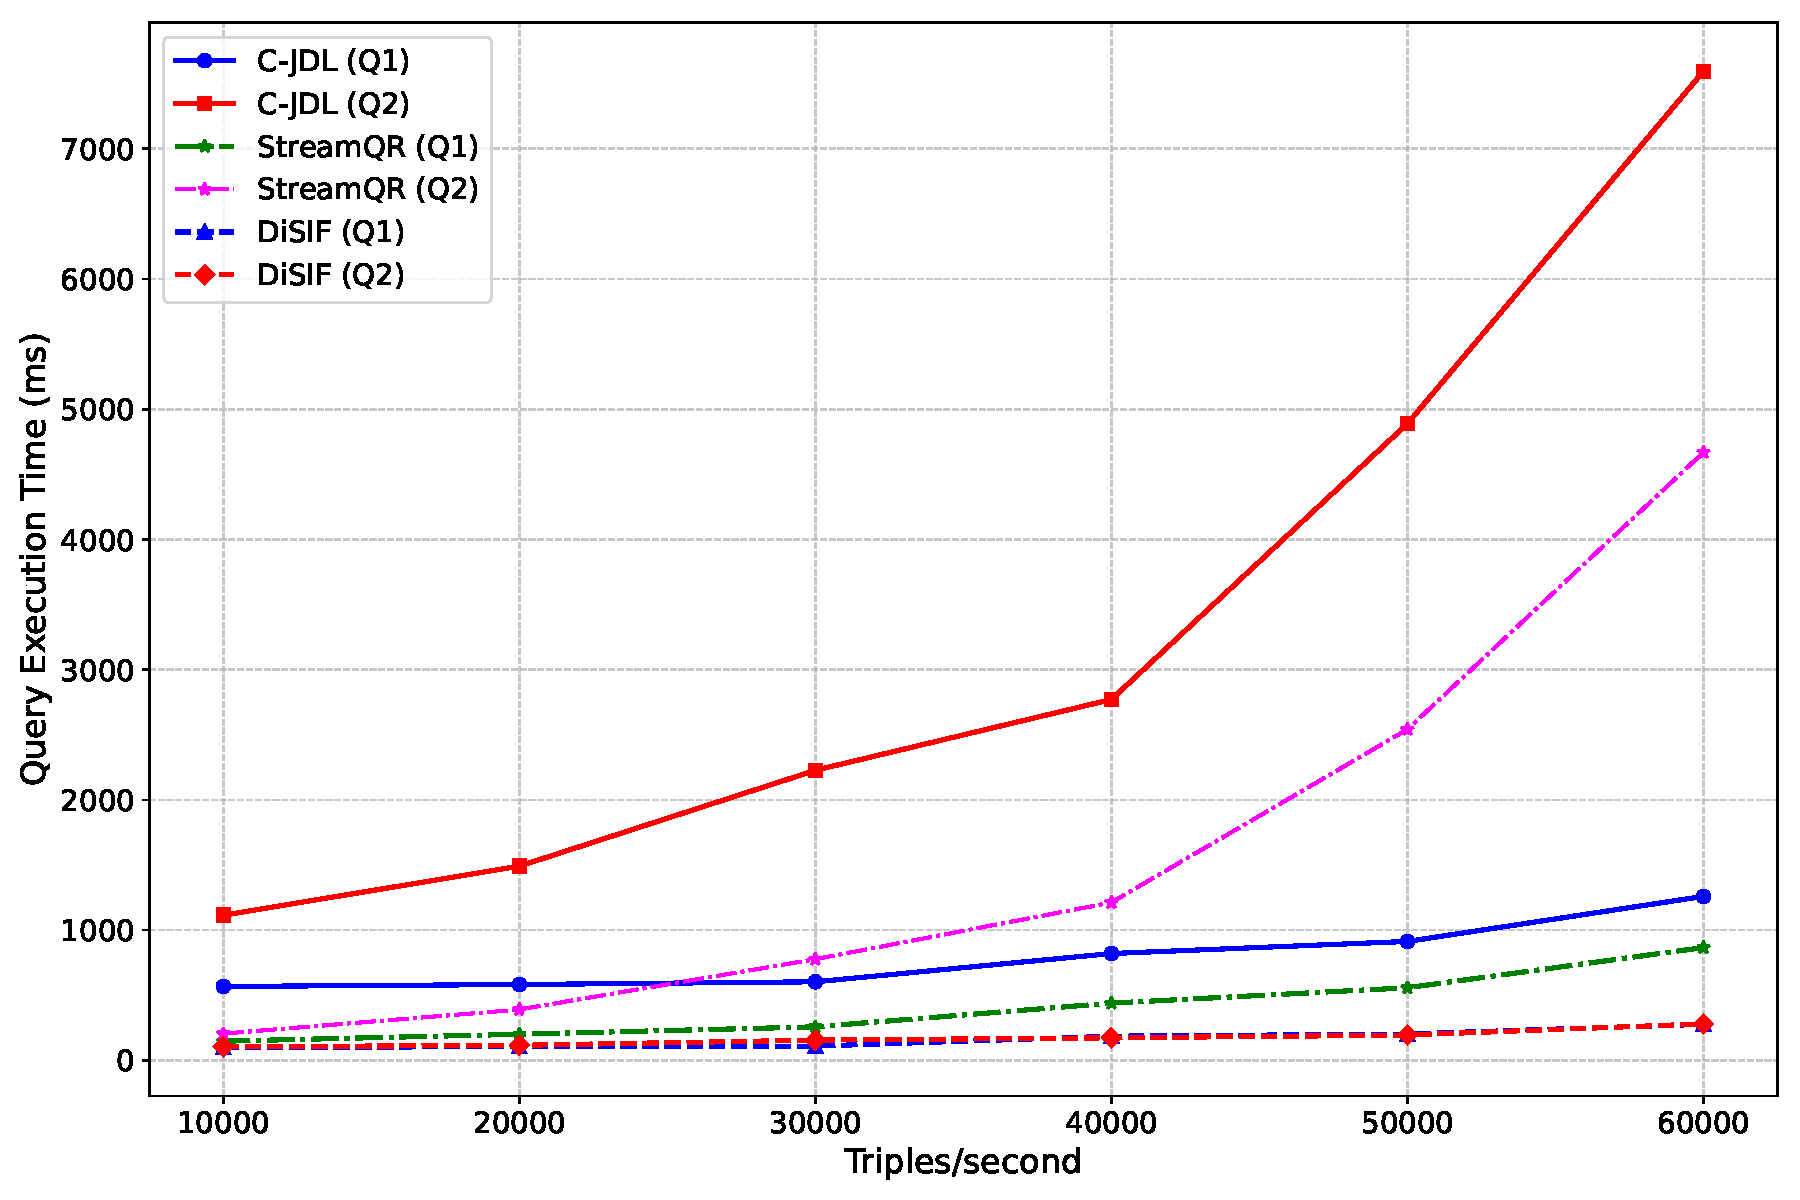
\includegraphics[width=\columnwidth]{Time_execution_Q1Q2_StreamQR_NonLogarithmicAdjustment_LinearScale_Q1Q2.pdf}
%     \subcaption{Comparing Execution Times for Q1 and Q2 in Centralized and Distributed Environments}
%     \label{fig:Timeexperiment1}
%   \end{subfigure}
%   \hfill
%   \begin{subfigure}{0.48\textwidth} % Same size for balance
%     \centering
%     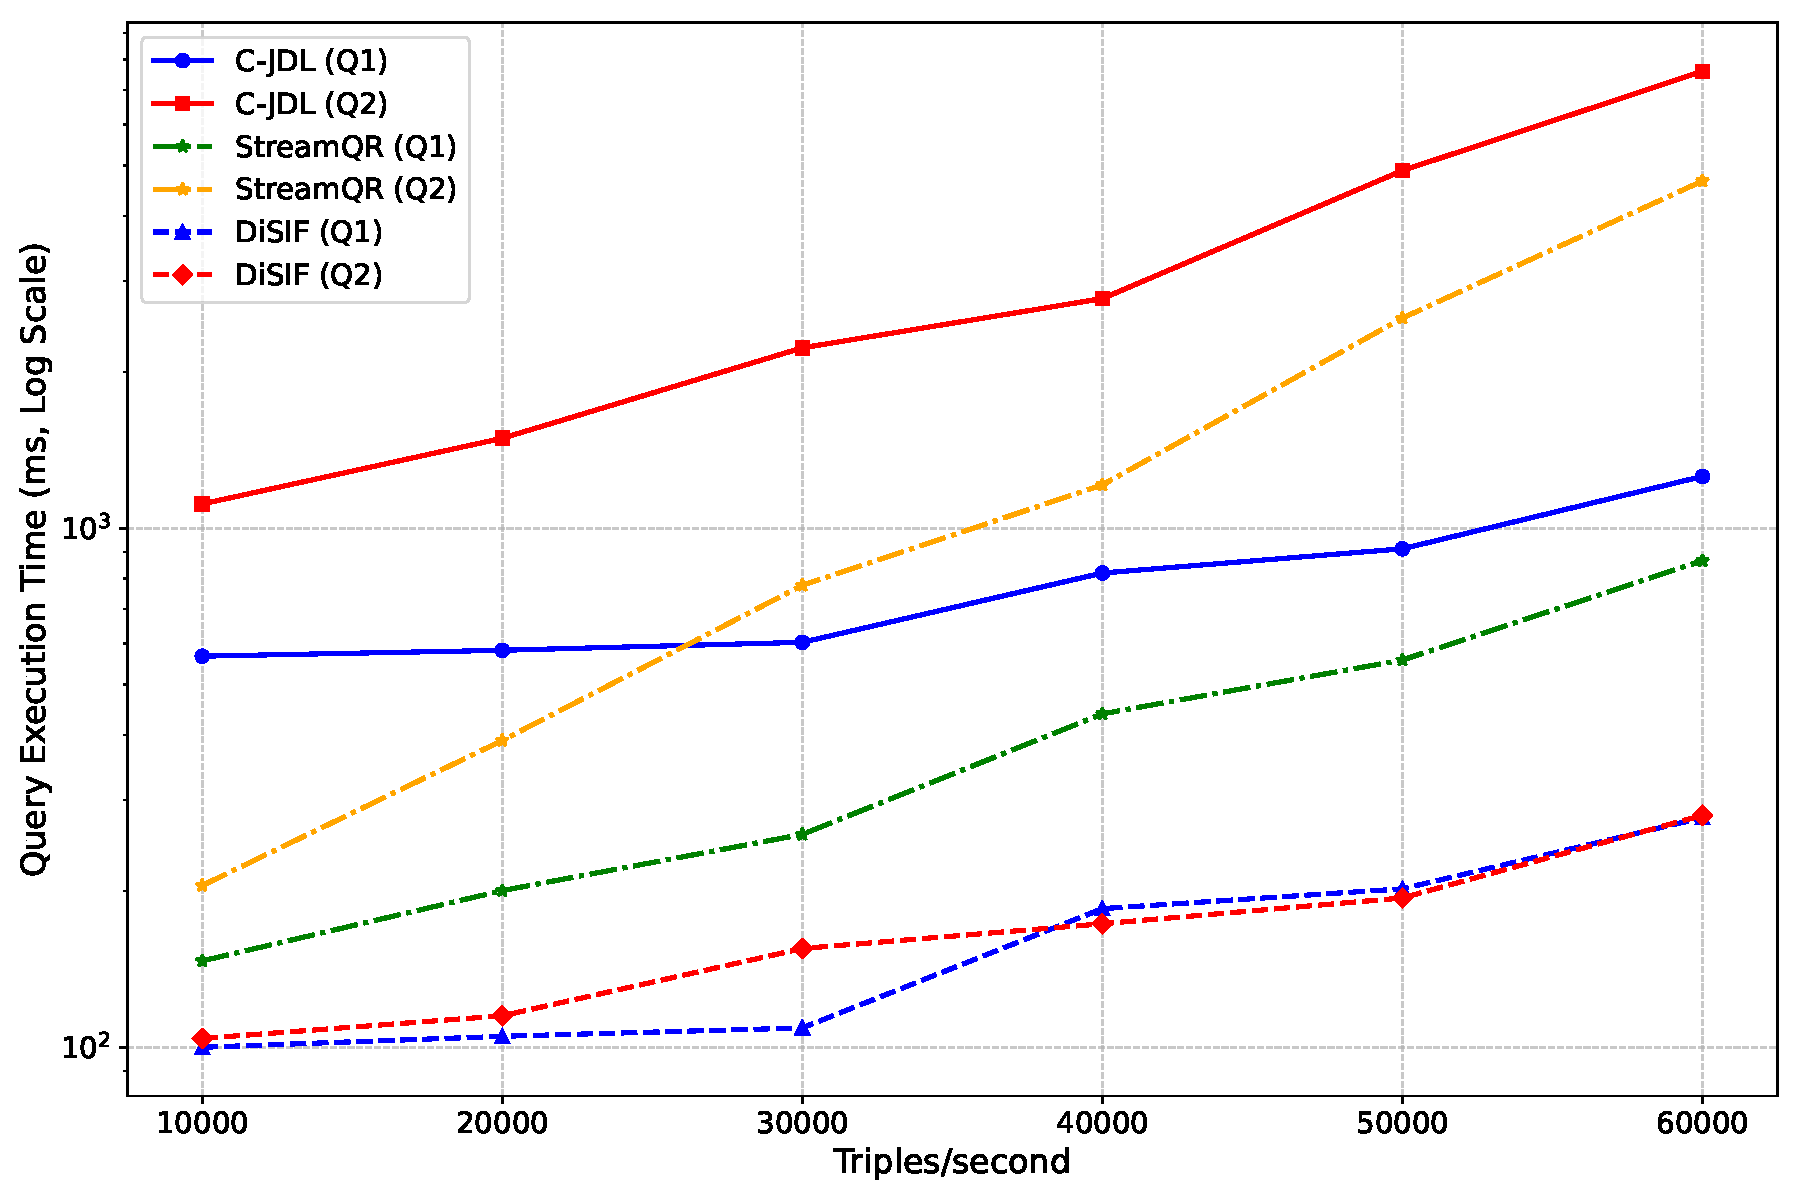
\includegraphics[width=\columnwidth]{Time_execution_Q1Q2_StreamQR_NonLogarithmicAdjustment_LogScale_Q1Q2.pdf}
%     \subcaption{Comparing Logarithmic Execution Times for Q1 and Q2 in Centralized and Distributed Environments}
%     \label{fig:Timeexperiment2}
%   \end{subfigure}

%   \vspace{1cm} % Vertical space between the row of subfigures
%   \begin{subfigure}{0.48\textwidth} % Use column width again for inline placement
%     \centering
%     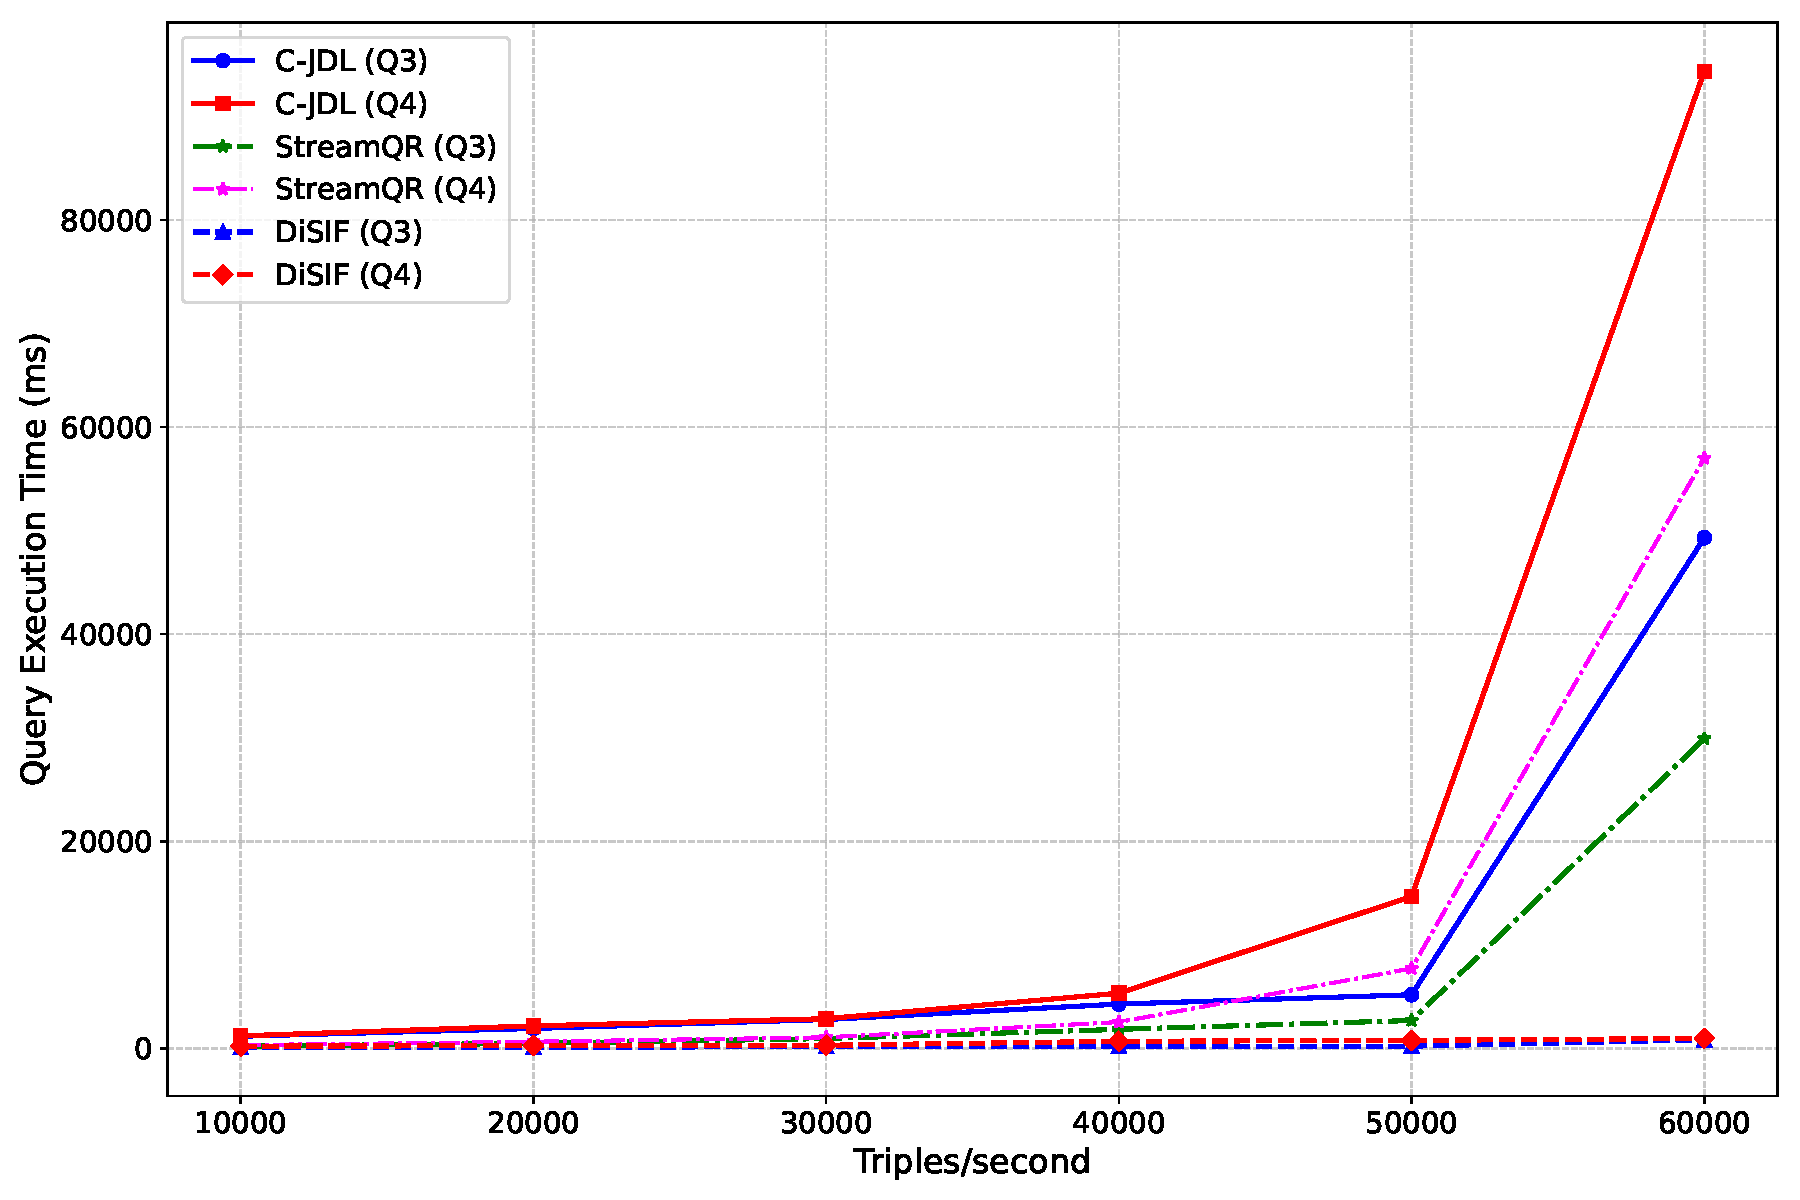
\includegraphics[width=\columnwidth]{Time_execution_Q1Q2_StreamQR_NonLogarithmicAdjustment_LinearScale_Q3Q4.pdf}
%     \subcaption{Comparing Execution Times for Q3 and Q4 in Centralized and Distributed Environments}
%     \label{fig:Timeexperiment3}
%   \end{subfigure}
%   \hfill
%   \begin{subfigure}{0.48\textwidth} % Keep consistency in size
%     \centering
%     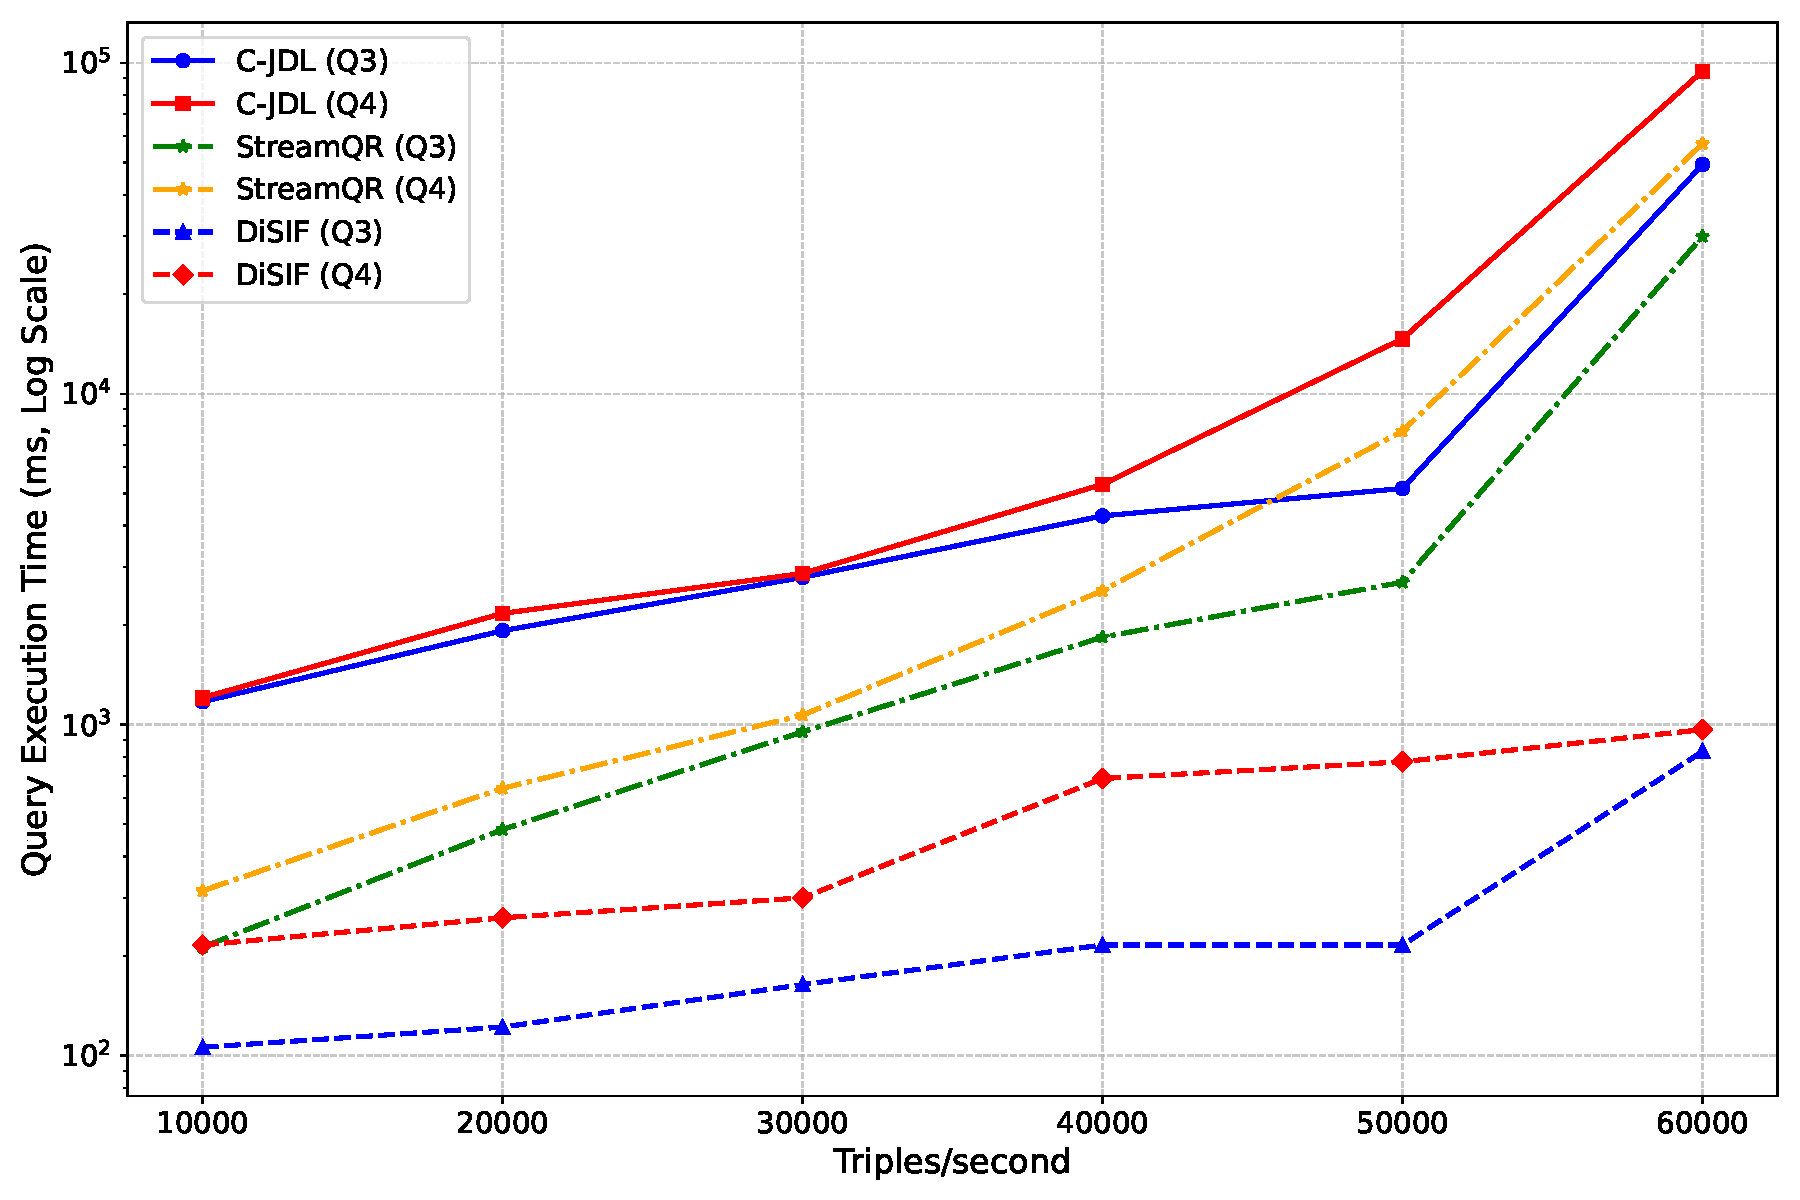
\includegraphics[width=\columnwidth]{Time_execution_Q1Q2_StreamQR_NonLogarithmicAdjustment_LogScale_Q3Q4.pdf}
%     \subcaption{Comparing Logarithmic Execution Times for Q3 and Q4 in Centralized and Distributed Environments}
%     \label{fig:Timeexperiment4}
%   \end{subfigure}
  
%   \caption{Query execution times in Centralized and Distributed Environments}
%   \label{fig:Timeexperiment1234}
% \end{figure}

\begin{figure}[t] % First figure
  \centering
  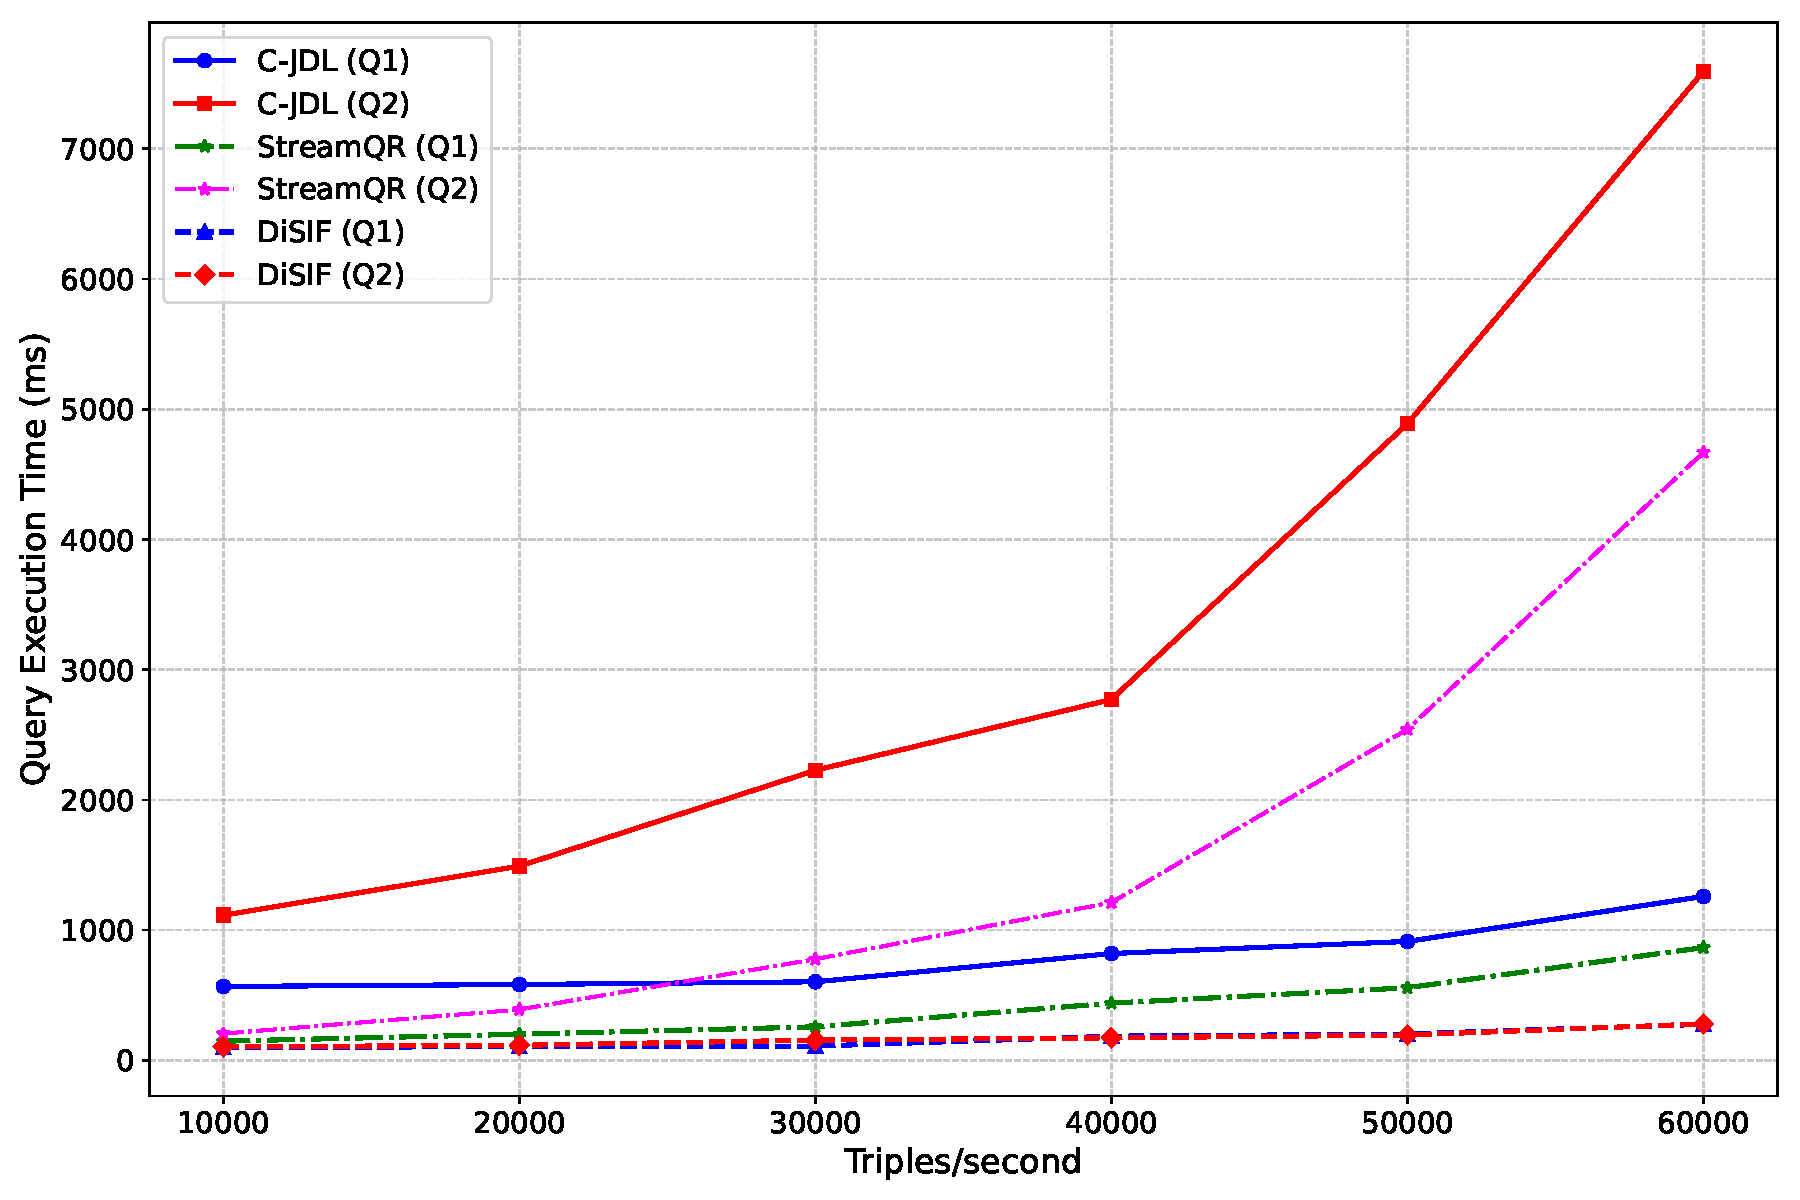
\includegraphics[width=0.8\columnwidth]{Time_execution_Q1Q2_StreamQR_NonLogarithmicAdjustment_LinearScale_Q1Q2.pdf}
  \caption{Comparing Execution Times for Q1 and Q2 in Centralized and Distributed Environments (Linear Scale)}
  \label{fig:Timeexperiment1}
\end{figure}

\begin{figure}[t] % Second figure
  \centering
  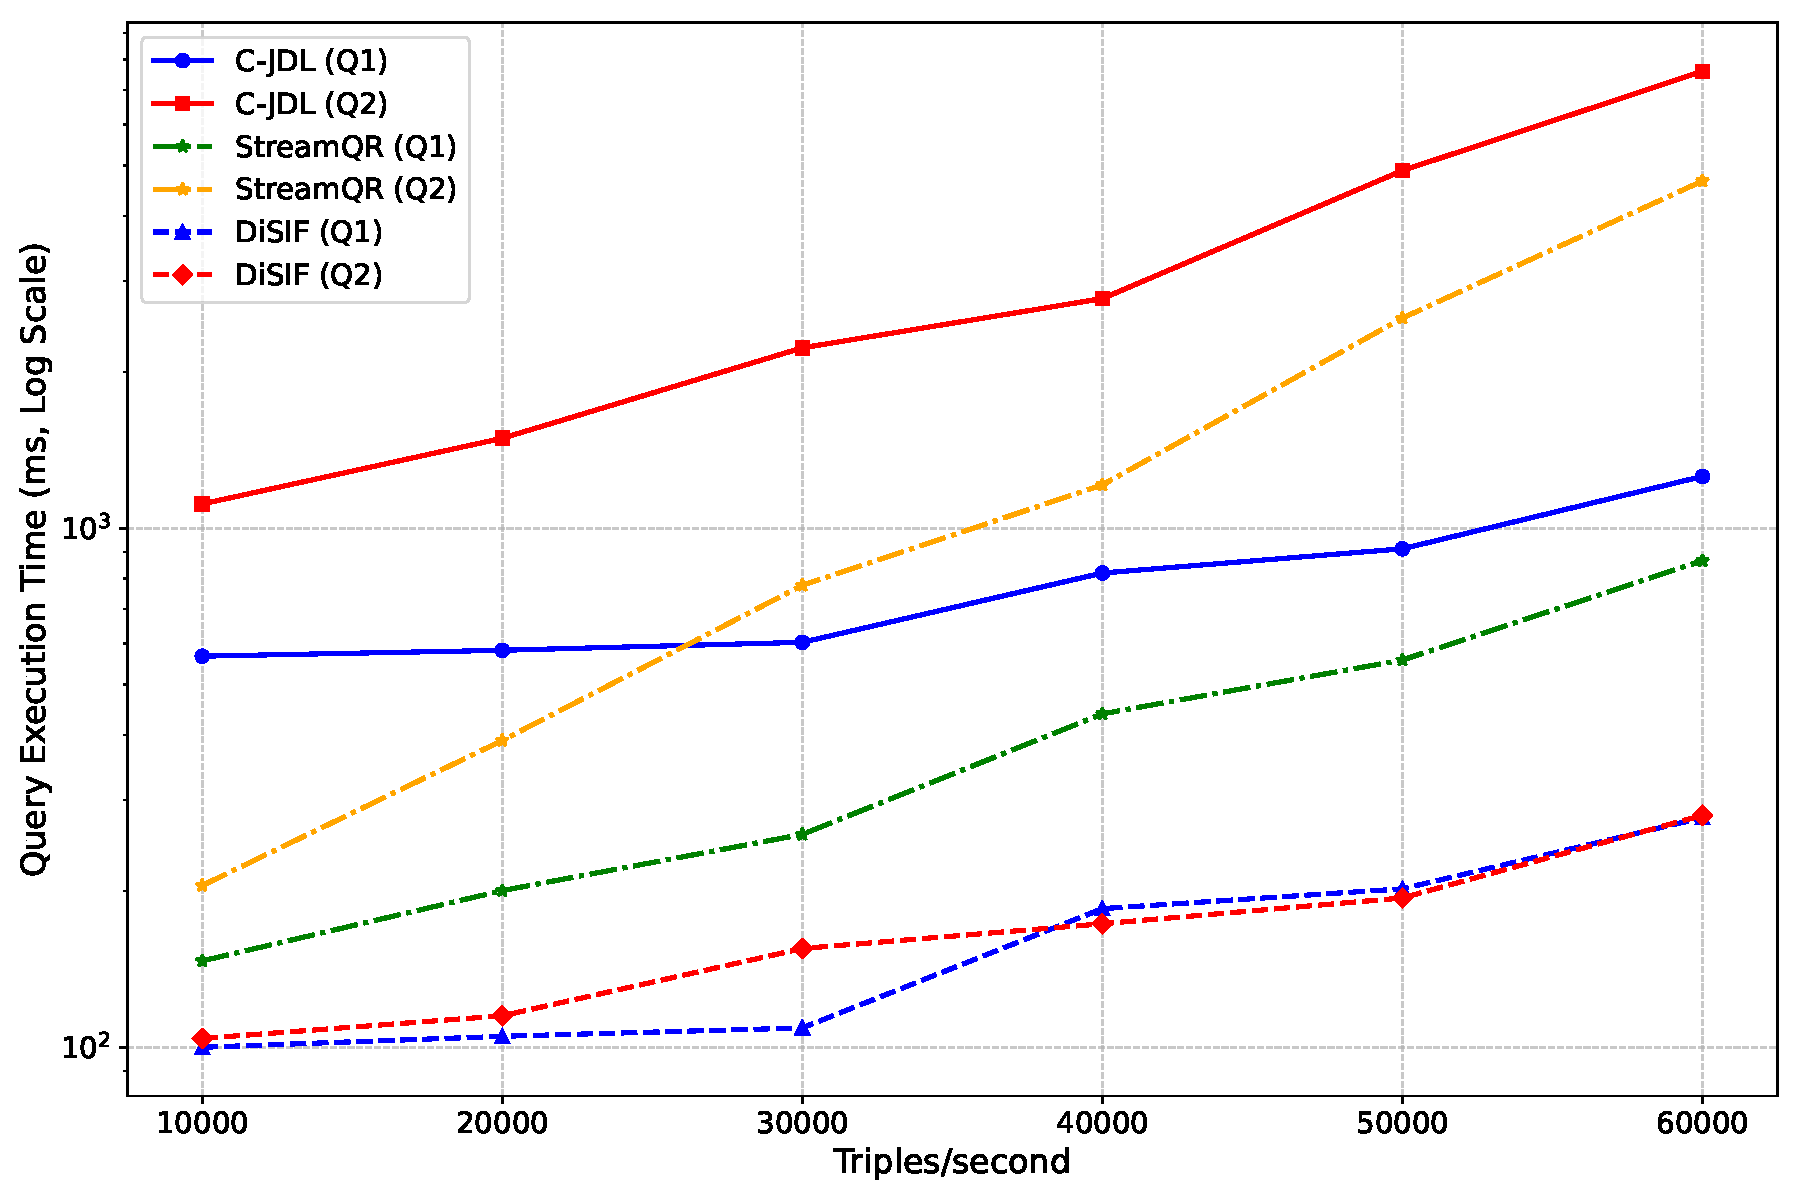
\includegraphics[width=0.8\columnwidth]{Time_execution_Q1Q2_StreamQR_NonLogarithmicAdjustment_LogScale_Q1Q2.pdf}
  \caption{Comparing Logarithmic Execution Times for Q1 and Q2 in Centralized and Distributed Environments}
  \label{fig:Timeexperiment2}
\end{figure}

\begin{figure}[t] % Third figure
  \centering
  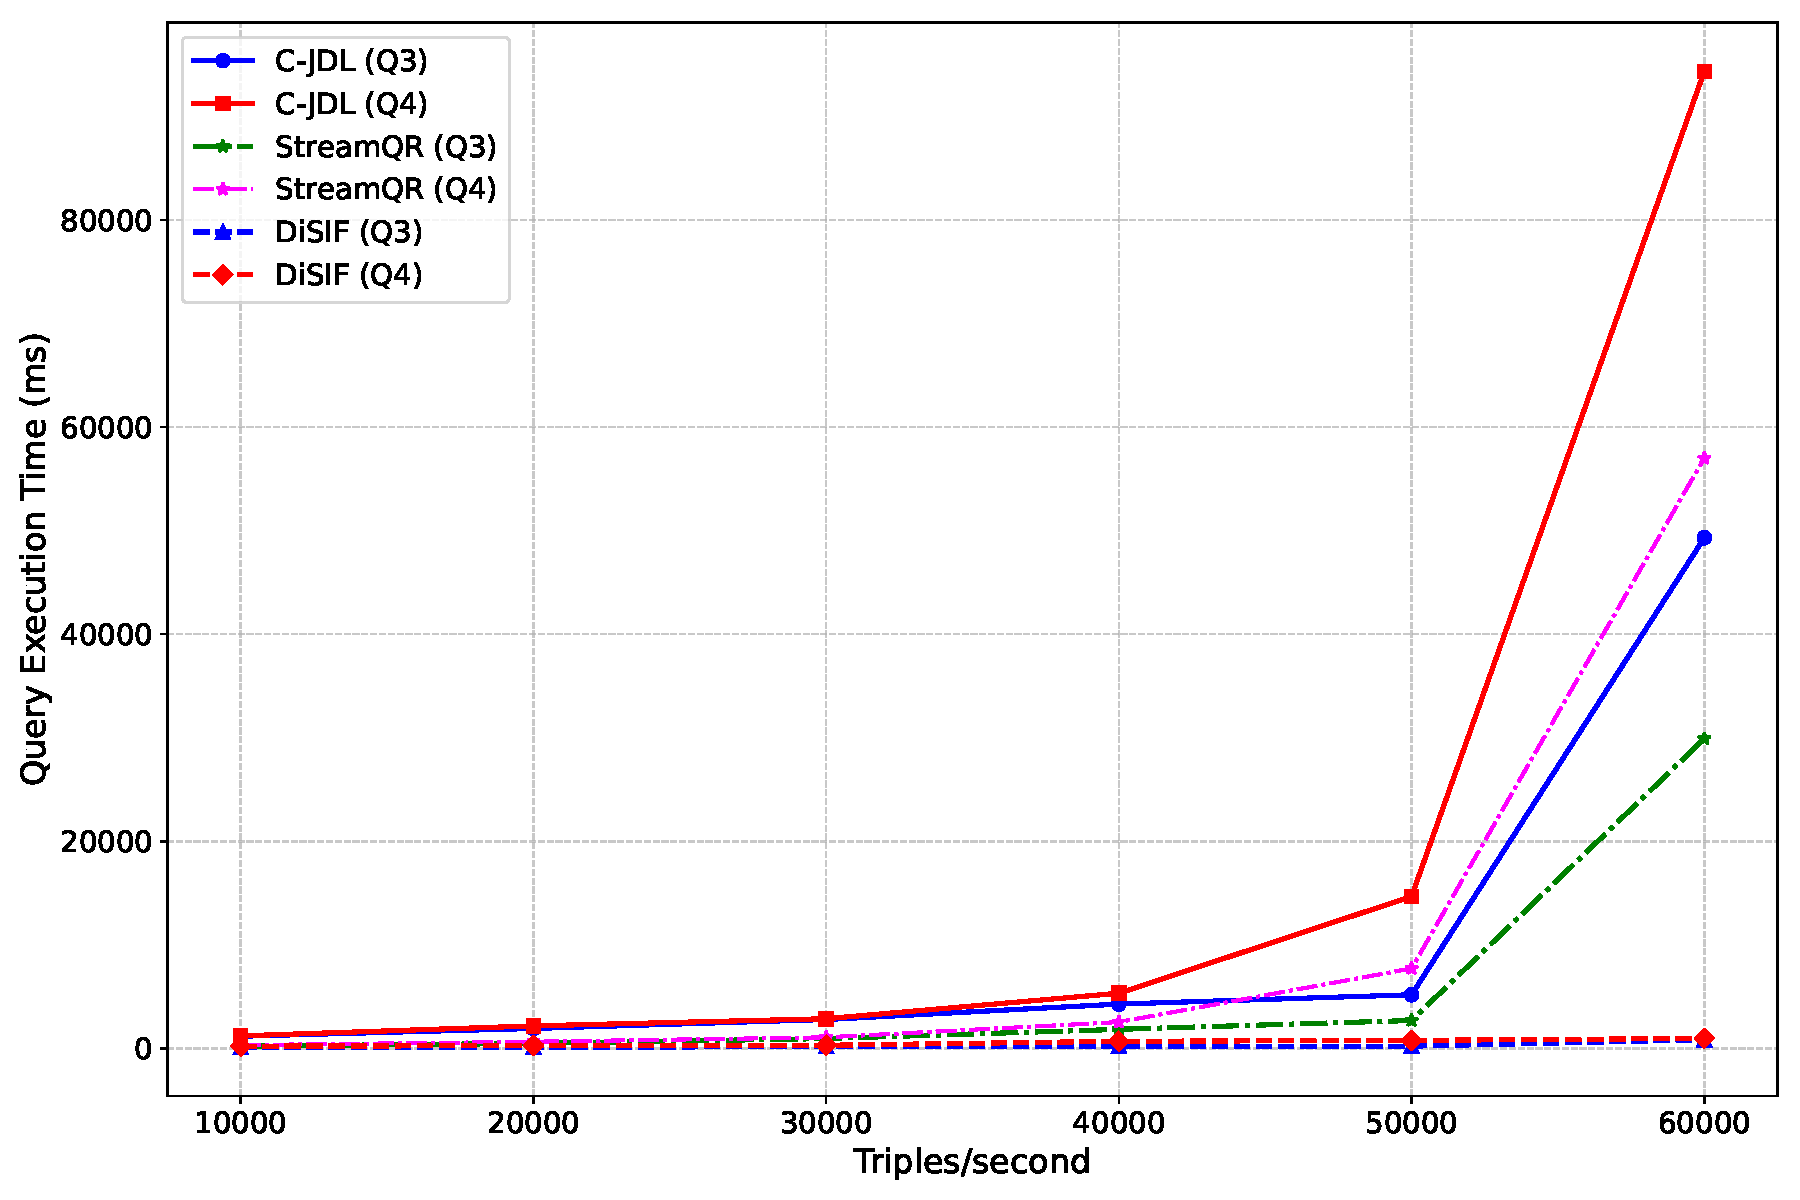
\includegraphics[width=0.8\columnwidth]{Time_execution_Q1Q2_StreamQR_NonLogarithmicAdjustment_LinearScale_Q3Q4.pdf}
  \caption{Comparing Execution Times for Q3 and Q4 in Centralized and Distributed Environments (Linear Scale)}
  \label{fig:Timeexperiment3}
\end{figure}

\begin{figure}[t] % Fourth figure
  \centering
  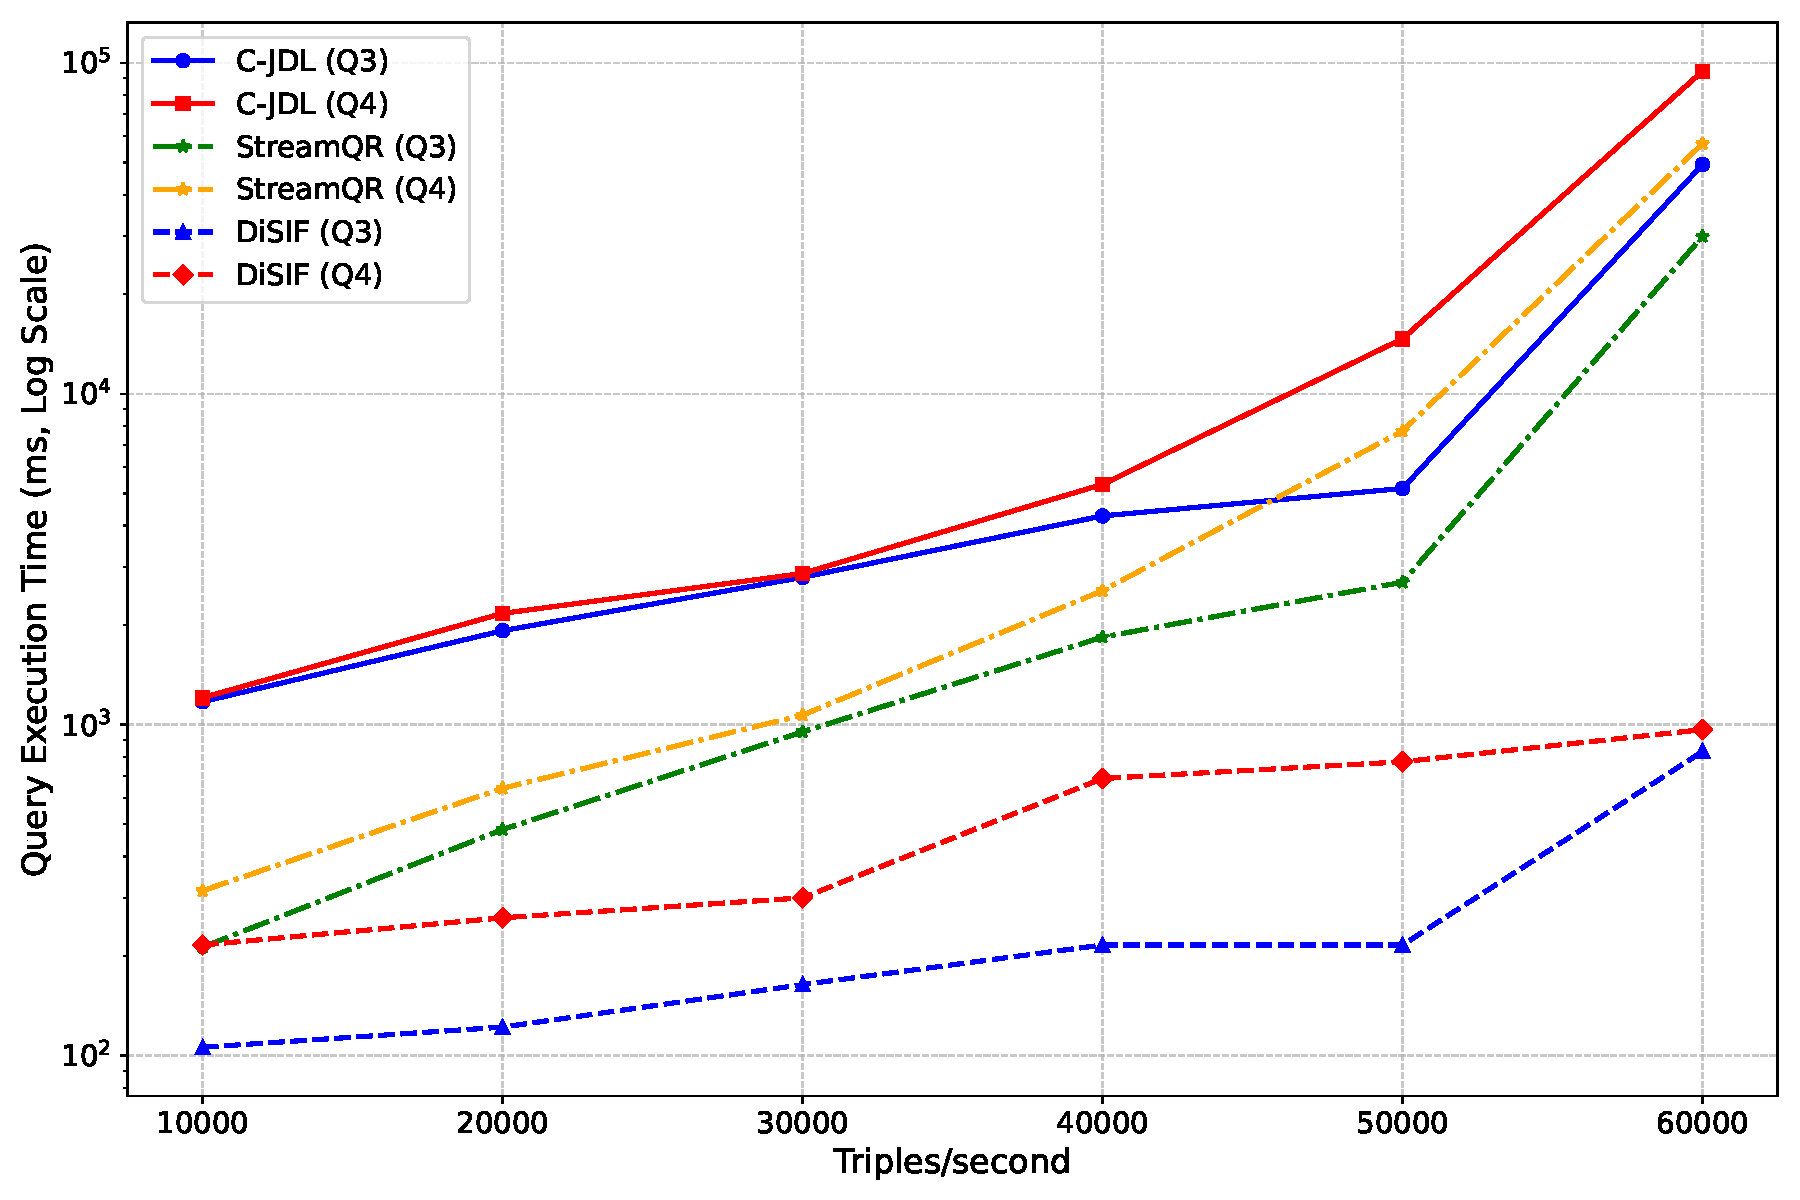
\includegraphics[width=0.8\columnwidth]{Time_execution_Q1Q2_StreamQR_NonLogarithmicAdjustment_LogScale_Q3Q4.pdf}
  \caption{Comparing Logarithmic Execution Times for Q3 and Q4 in Centralized and Distributed Environments}
  \label{fig:Timeexperiment4}
\end{figure}






To analyze the execution time for queries $Q_1$ to $Q_4$ and subsequently query $Q_m$, Figures \ref{fig:Timeexperiment1},\ref{fig:Timeexperiment2},
\ref{fig:Timeexperiment3} and \ref{fig:Timeexperiment4} illustrates the results for various data transmission rates (triples per second).
 This analysis compares both the centralized JDL (C-JDL), StreamQR and DiSIF approaches.


In the C-JDL model, all queries, including $Q_1$, $Q_2$, $Q_3$, or $Q_4$, and $Q_m$, are executed sequentially
 on the master node. For example, during the time analysis of queries $Q_1$ to $Q_4$ and $Q_m$,
  all raw data is sent from the worker nodes to the master node, where the queries are processed.
  This centralized structure leads to exponential growth in query execution time,
   especially for more complex queries (like $Q_3$ and $Q_4$), as the data transmission rate (triples/sec)
    increases. This increase is due to $Q_m$’s dependency on the output of $Q_3$ and $Q_4$,
     both of which must be processed on the master node.
      As a result, the C-JDL method exhibits the longest query execution time and has relatively poor
       performance in terms of latency and efficiency.

In the StreamQR model, queries are aggregated and executed as a single large query,
 which significantly improves execution time compared to the C-JDL method.
  Since all queries are aggregated and executed in one process, the sequential execution
   is eliminated, and processing speed increases. However, as the data transmission rate
    increases, particularly at higher rates, the complexity and size of the aggregated query
     grow, and its execution time gradually increases. At high rates, the execution time
      of StreamQR may approach that of C-JDL, especially when the aggregated query
       becomes very complex and large.


In the DiSIF model, queries are executed locally the worker nodes within the fog layer,
 and only the processed results are sent to the master node.
  This significantly reduces query execution time, as parallel processing occurs
   on the worker nodes, with only the final aggregation (via the execution of query $Q_m$)
    performed on the master node. Unlike the previous methods, DiSIF has the shortest query
     execution time, as it leverages distributed processing across the network rather than
      relying on a single central node, resulting in much better efficiency.




As observed in Figure \ref{fig:Timeexperiment1} and \ref{fig:Timeexperiment2},
 the execution time of DiSIF(Q1), StreamQR(Q1) and C-JDL(Q1) increases almost linearly
  with the increase in the data sending rate. Moreover,
   the time needed for executing DiSIF(Q1) is generally less compared
    to others, and this time difference remains approximately constant across various data
     sending rates.


Figures \ref{fig:Timeexperiment3} and \ref{fig:Timeexperiment4} reveal an exponential
 increase in execution time for queries C-JDL(Q3), StreamQR(Q3), C-JDL(Q4) and StreamQR(Q4)
  as the data sending rate rises. In contrast, the execution time for DiSIF(Q3)
   and DiSIF(Q4) shows a much less significant growth rate. This discrepancy is due
    to the dependency of query $Q_m$ on $Q_3$ and $Q_4$. When both queries are executed
     on the master node (centralized mode), the delay becomes substantially higher.
      In the DiSIF model, however, queries $Q_3$ and $Q_4$ are processed on the worker nodes
      , and only the results are sent to the master node, 
      thereby reducing delays associated with producing results for $Q_m$.
This illustrates the stability or robustness of the DiSIF method.


\end{itemize} 



\subsection{Network load perspective}


Next, we compare C-JDL, StreamQR and DiSIF approaches
 in terms of the number and volume of messages transmitted across the network (network load).

In a centralized approach (C-JDL and StreamQR), the total load \(L_c\) is given by the sum
 of all raw data \(D_i\) sent from each worker node \(i\) to the master node:

\begin{equation}
    L_c = \sum_{i \in N} D_i
    \end{equation}

Here, \(D_i\) represents the raw data transmitted from worker node \(i\) to the master node.

In DiSIF approach, the total load \(L_d\) is given by the sum of all results \(R_i\)
 obtained by each worker node \(i\) and sent to the master node:


\begin{equation}
    L_d = \sum_{i \in N} R_i
\end{equation}
    
In this case, \(R_i\) represents the results obtained by worker node \(i\)
 that are transmitted to the master node.

As can be seen from these expressions, for large data transmission, \(L_c\)
 is significantly greater than \(L_d\). Therefore, in the centralized approaches,
  the network load is high due to the transfer of all raw data from the worker nodes
   to the master node, whereas in DiSIF approach, the network load is minimized by transferring
    only the processed results.




An example of a raw RDF message used in the Kafka system for sending from worker nodes To
 the master node is as follows:

\small
\begin{quote}
\begin{verbatim}
https://www.wtlab.com/TrafficStream/vehicle37450
	 http://www.w3.org/2003/01/geo/wgs84_pos
   #location
	 7103


https://www.wtlab.com/TrafficStream/vehicle37450 
	http://example.org/timestamp 
	2023-09-20T12:00:028948


https://www.wtlab.com/TrafficStream/vehicle37450
	http://example.org/speed
	75^^http://www.w3.org/2001/XMLSchema#int
\end{verbatim}
\end{quote}

\normalsize % Return to normal size
Each raw message consists of 317 characters, and its size is 311 bytes. Additionally,
 an example of the output message obtained from queries $Q_1$ to $Q_4$, which is sent from worker
  nodes to the master node in DiSIF approach, is as follows:

\small
\begin{quote}
\begin{verbatim}
"7103 congestion"
\end{verbatim}
\end{quote}

\normalsize % Return to normal size


This message contains 15 characters and 14 bytes.
 In Figure \ref{fig:networkLoad}, the network usage
 for sending messages for various queries in C-JDL, StreamQR and DiSIF approaches is illustrated.




\begin{figure}[t]
  \centering
  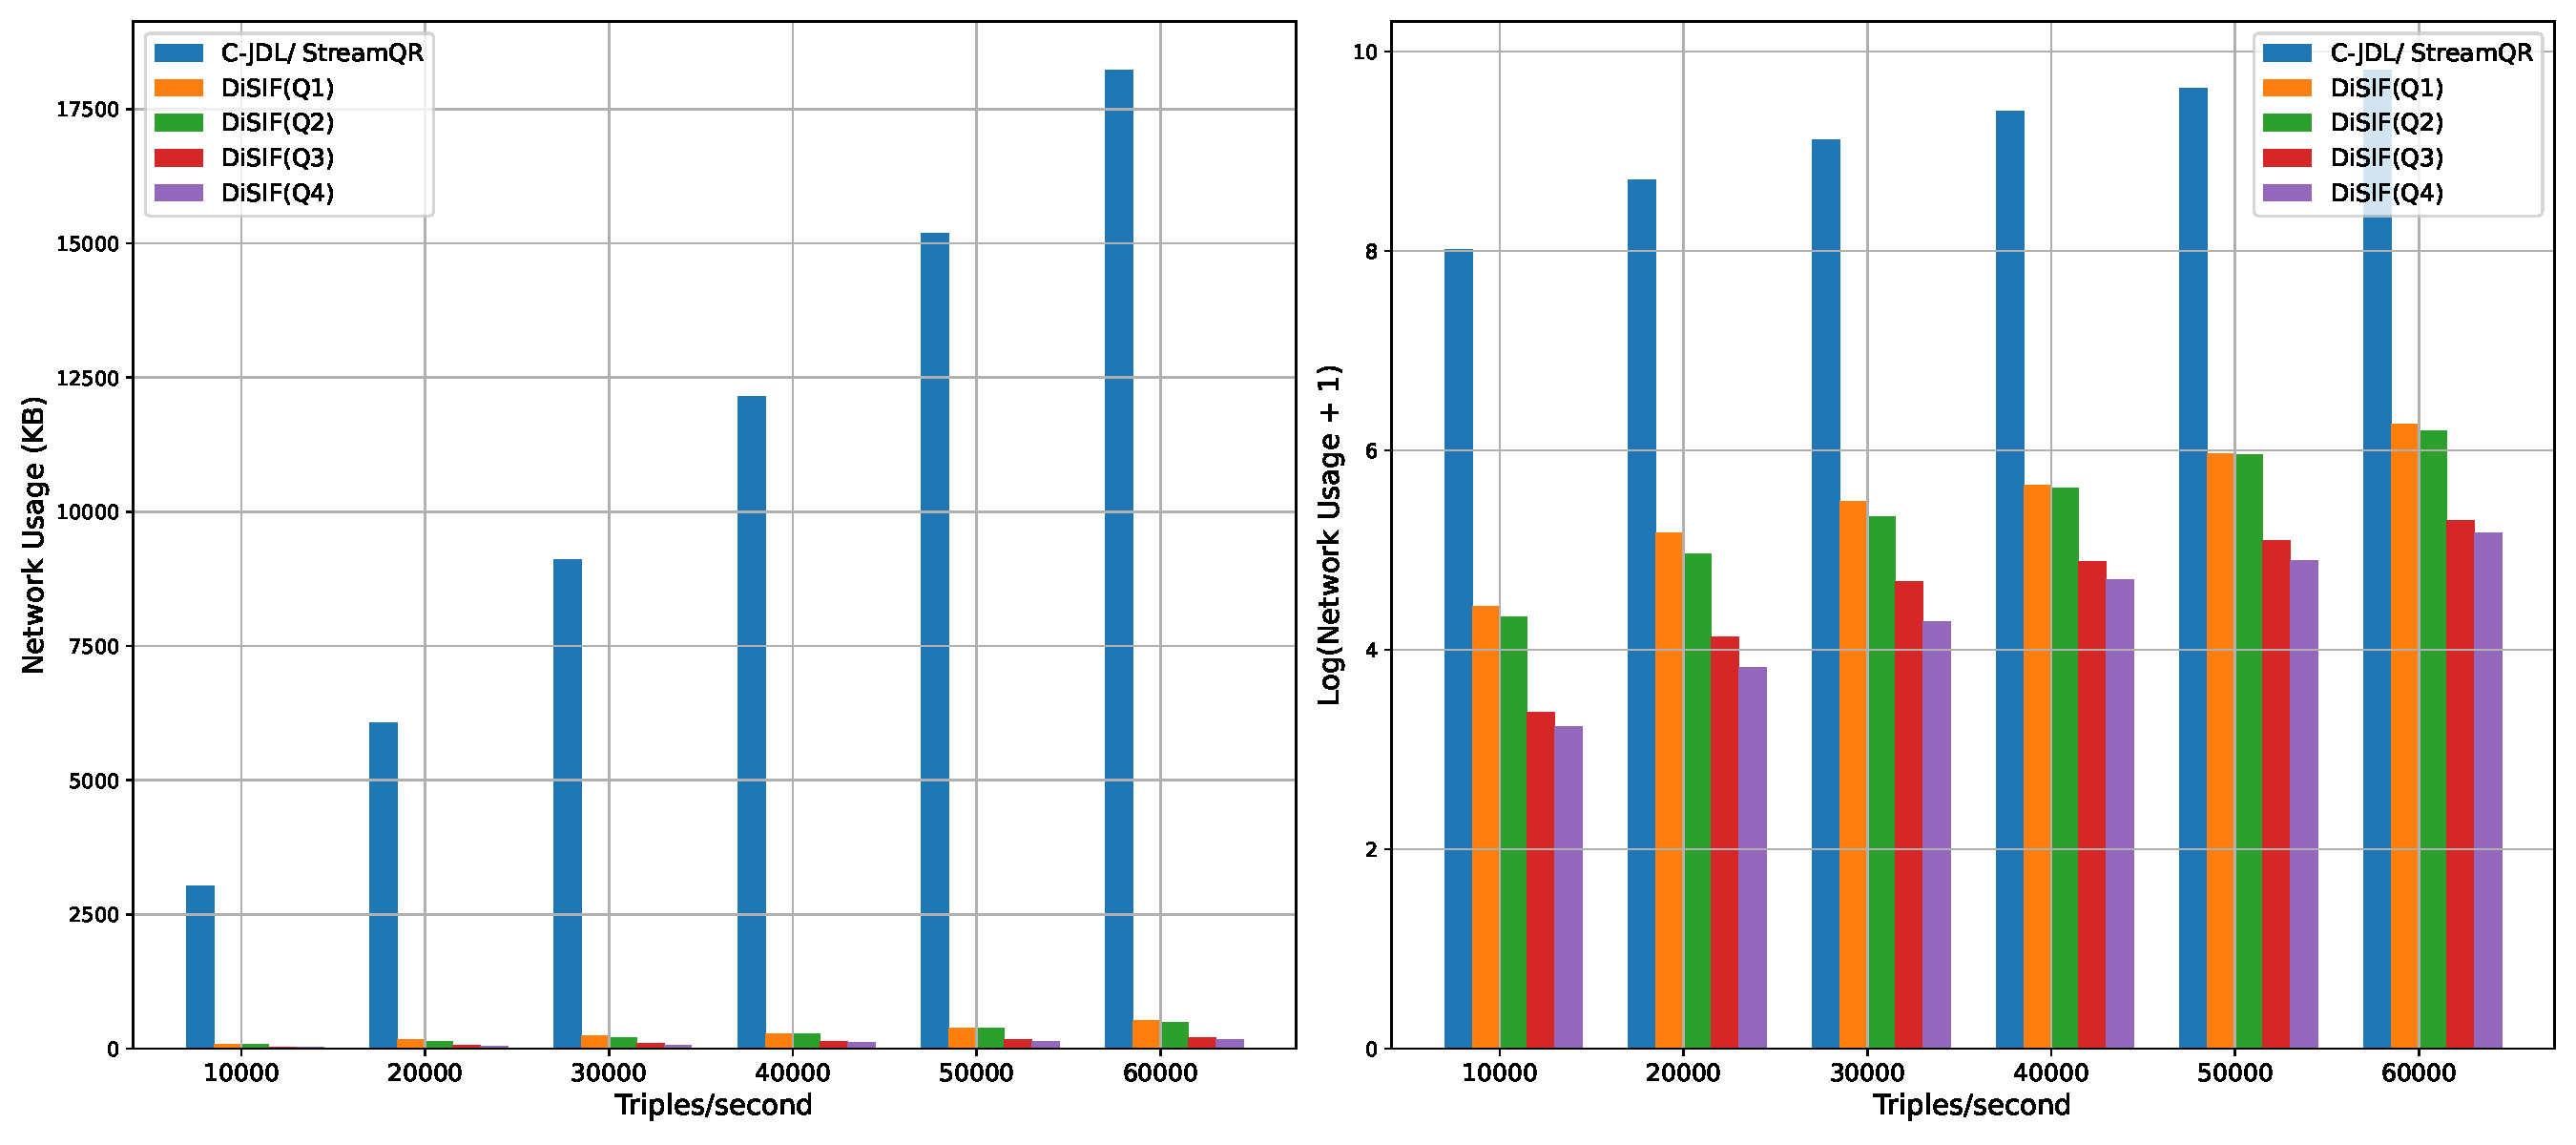
\includegraphics[width=0.5\textwidth]{Network_Usage_vs_Log_vs_Triples.pdf}
  \caption{Network usage comparison for different stream rates}
  \label{fig:networkLoad}
\end{figure}




As observed in Figure \ref{fig:networkLoad} , the volume of messages sent over the 
network wih Kafka in the C-JDL/StreamQR approaches is significantly higher compared
 to DiSIF approach.


In C-JDL/StreamQR approaches, all raw RDF data must be transmitted from worker nodes to
 the master node, resulting in a substantial network load. 
In contrast, the DiSIF method involves performing local computations and query executions
 on the worker nodes, with only the processed results—comprising much smaller message
  volumes—being transmitted to the master node.

Furthermore, as the data streaming rate increases, the number of messages sent also rises,
 highlighting the distinction between C-JDL/StreamQR approaches and DiSIF. 
Additionally, as the complexity of the queries increases  ($Q_1$< $Q_2$< $Q_3$< $Q_4$),
 fewer messages are sent in the network. In contrast, with C-JDL/StreamQR approaches,
  there is no significant difference in the volume of sent messages with respect to the
   complexity of the queries.



\subsection{Memory Consumption Perspective}


In terms of memory consumption, we employ the following two formulas to calculate the memory requirements for executing query $Q_m$ in both centralized and distributed approaches:

\begin{equation}
\text{Mem}_c(Q_i) = M_{Q_i Q_m} > M_{Q_i} + M_{Q_m}
\end{equation}

\begin{equation}
\text{Mem}_d(Q_i) = \max(M_{Q_i}, M_{Q_m})
\end{equation}

As observed, $M_{Q_i Q_m}$ signifies the amount of memory required when executing $Q_m$ and $Q_i$ sequentially on a master node. In both approaches, memory consumption for data transmission is neglected.

In the centralized approach, the sequential execution of queries $Q_i$ and $Q_m$ results in the generation of intermediate data in the memory of the master node. This leads to higher memory consumption ($\text{Mem}_c(Q_i Q_m)$) compared to the sum of individual memory consumptions ($M_{Q_i} + M_{Q_m}$).

However, in the distributed approach, since queries $Q_i$ and $Q_m$ are executed in parallel on different nodes, the memory consumption is equal to the maximum of the memory requirements for $Q_i$ and $Q_m$ in both worker and master nodes.

Next, we will analyze the distributed and centralized JDL methods in terms of memory
 consumption for executing query $Q_m$ on the master node.
%======================
\begin{figure}[t] % First figure
  \centering
  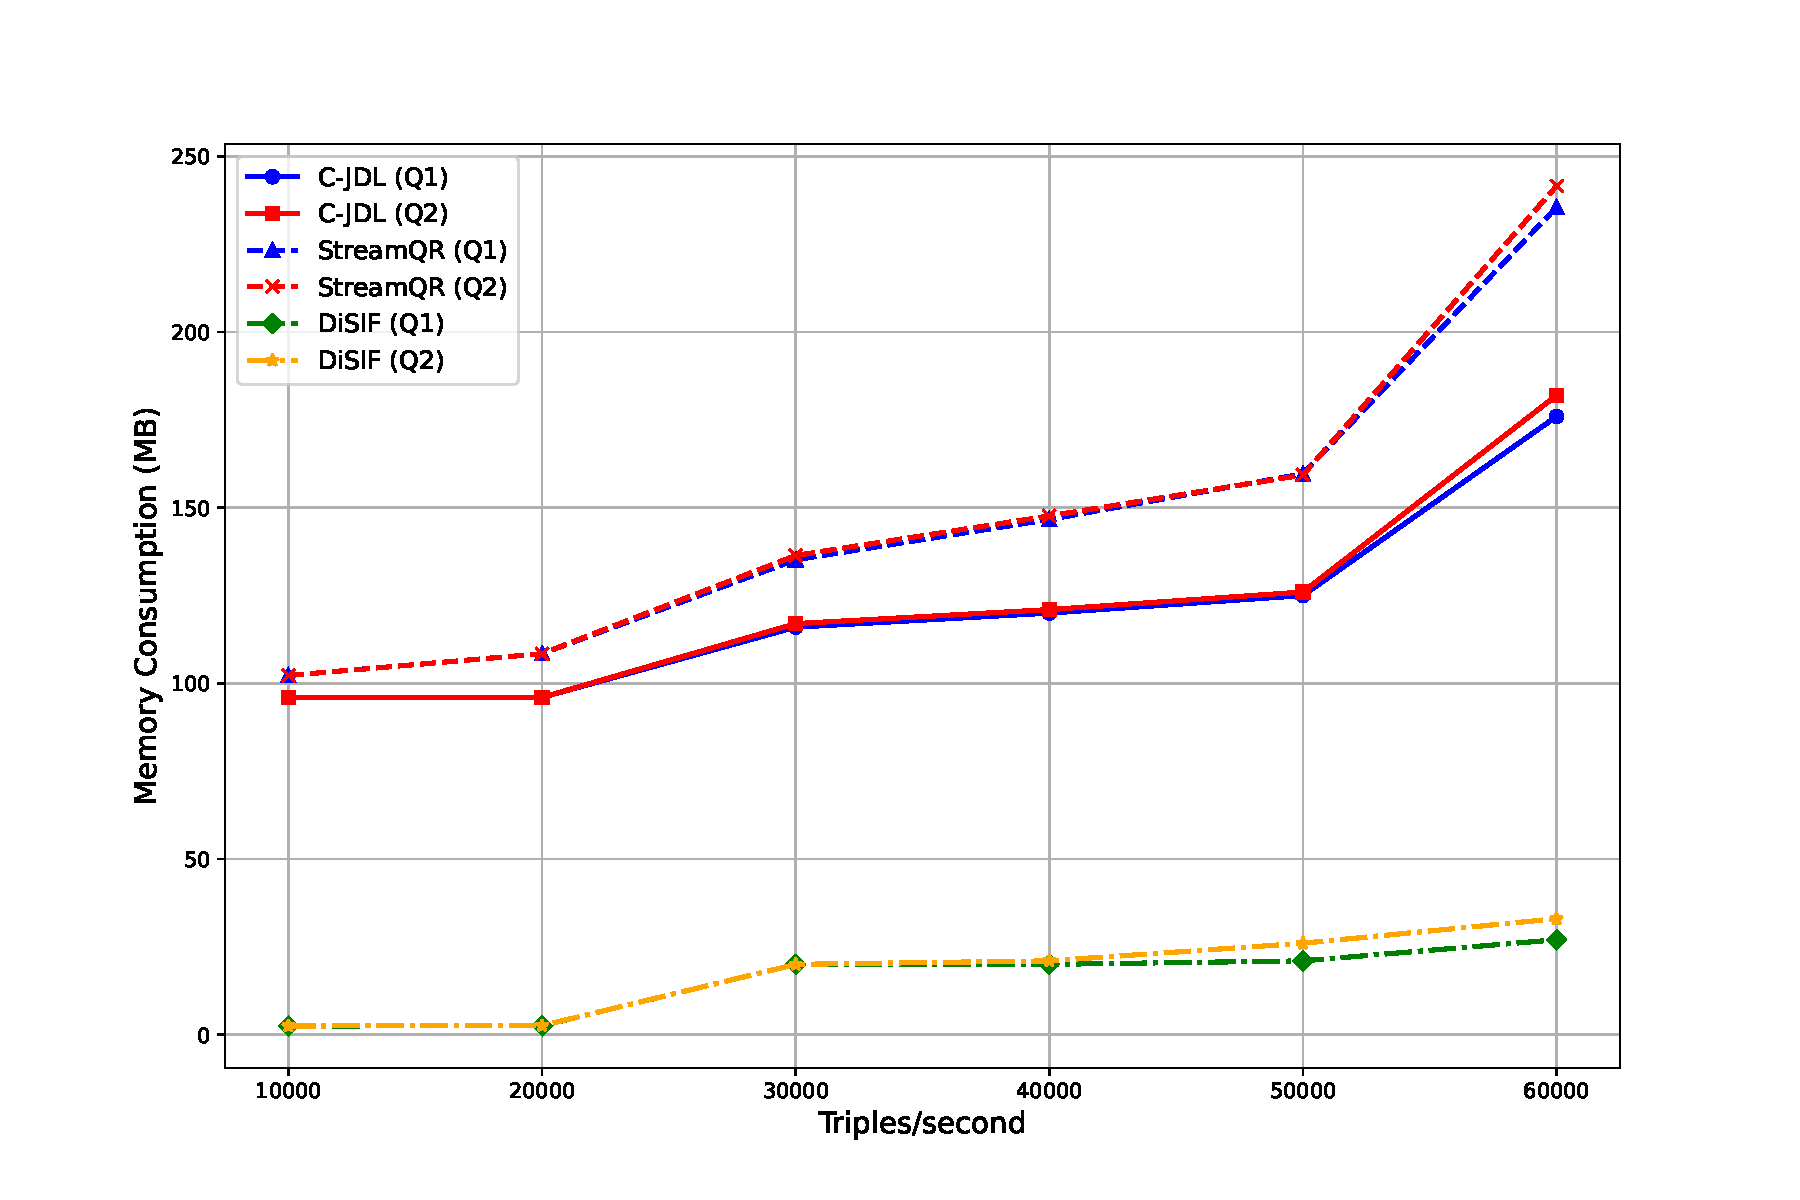
\includegraphics[width=0.8\columnwidth]{Memory_Consumption_vs_Stream_Rate_Linear_Enhanced_Q1Q2.pdf}
  \caption{Memory consumption for a single stream receiver node (Linear Scale) for Q1 and Q2}
  \label{fig:Memexperiment1}
\end{figure}

\begin{figure}[t] % Second figure
  \centering
  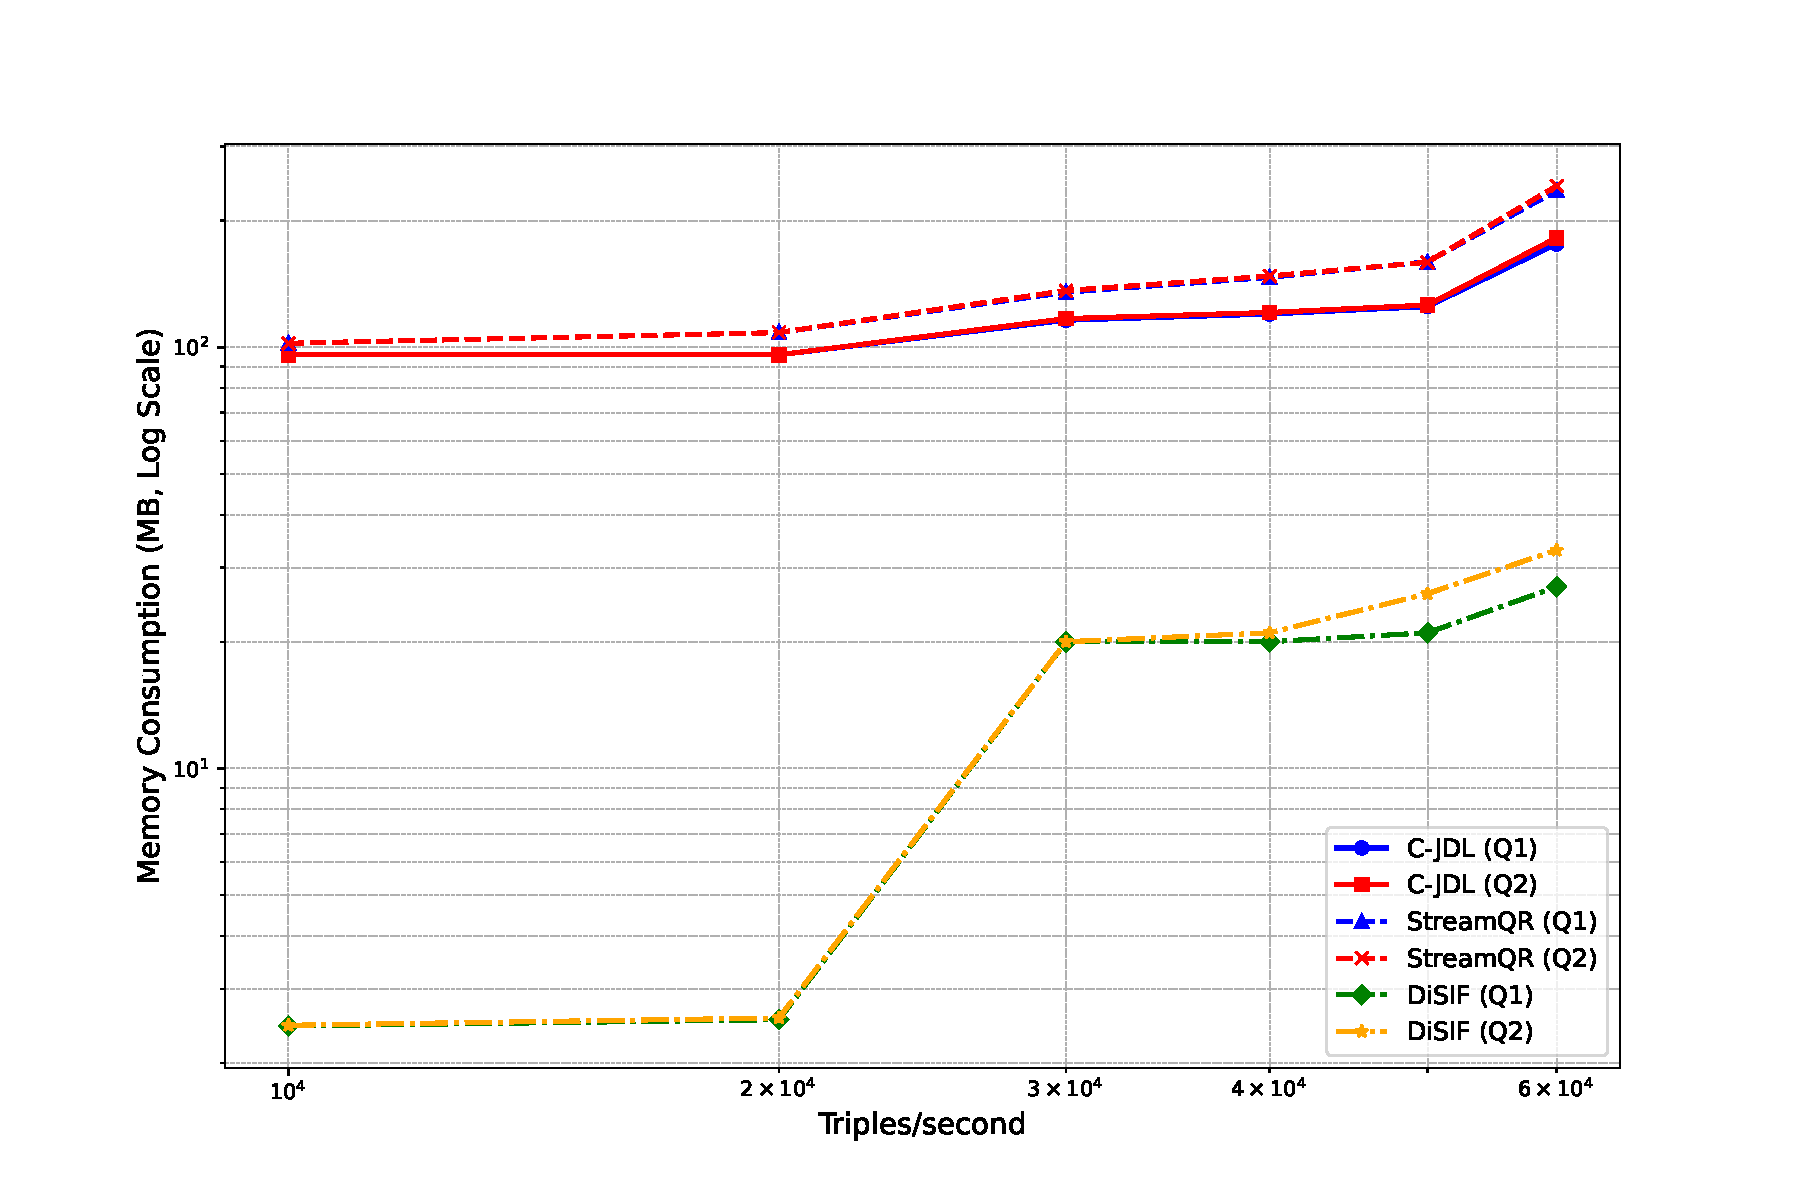
\includegraphics[width=0.8\columnwidth]{Memory_Consumption_vs_Stream_Rate_Log_Enhanced_Q1Q2.pdf}
  \caption{Memory consumption for a single stream receiver node (Log Scale) for Q1 and Q2}
  \label{fig:Memexperiment11}
\end{figure}

\begin{figure}[t] % Third figure
  \centering
  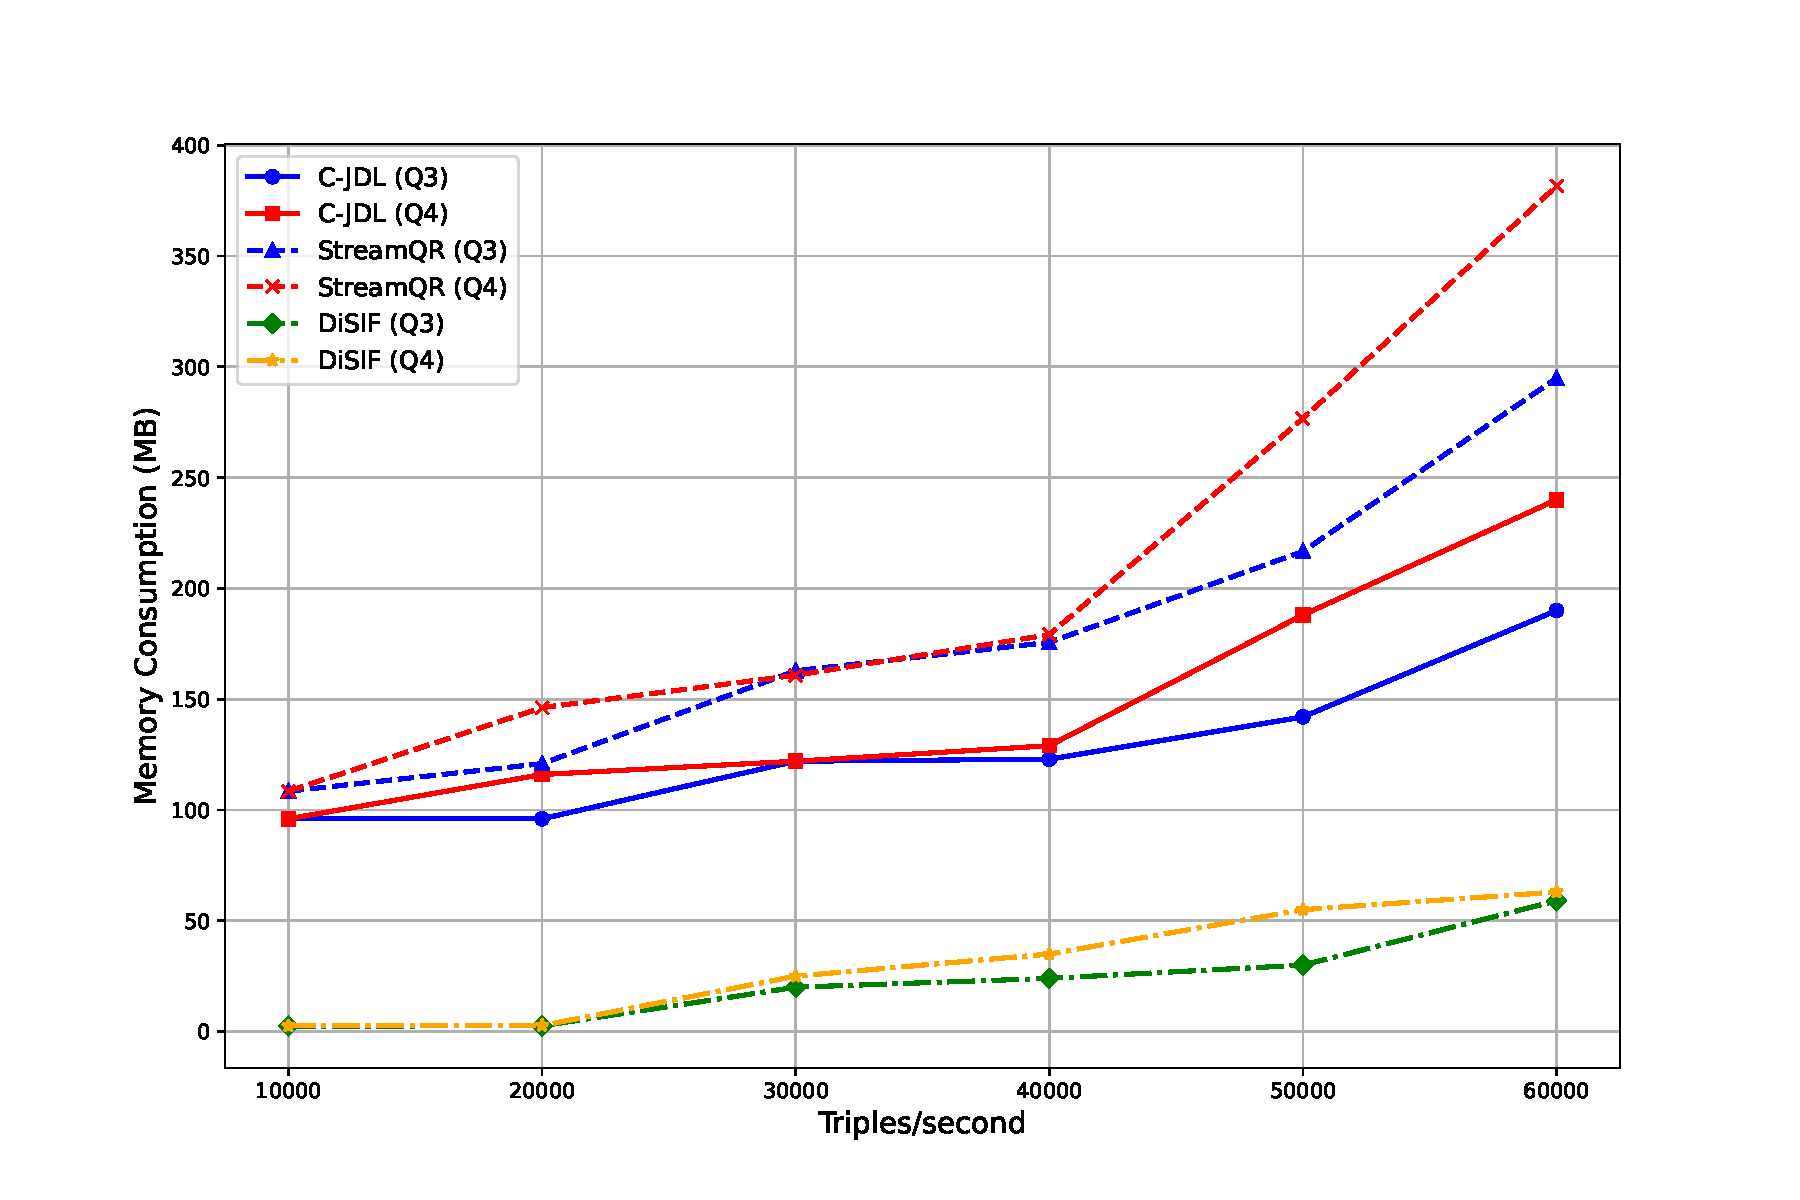
\includegraphics[width=0.8\columnwidth]{Memory_Consumption_vs_Stream_Rate_Linear_Enhanced_Q3Q4.pdf}
  \caption{Memory consumption for a single stream receiver node (Linear Scale) for Q3 and Q4}
  \label{fig:Memexperiment2}
\end{figure}

\begin{figure}[t] % Fourth figure
  \centering
  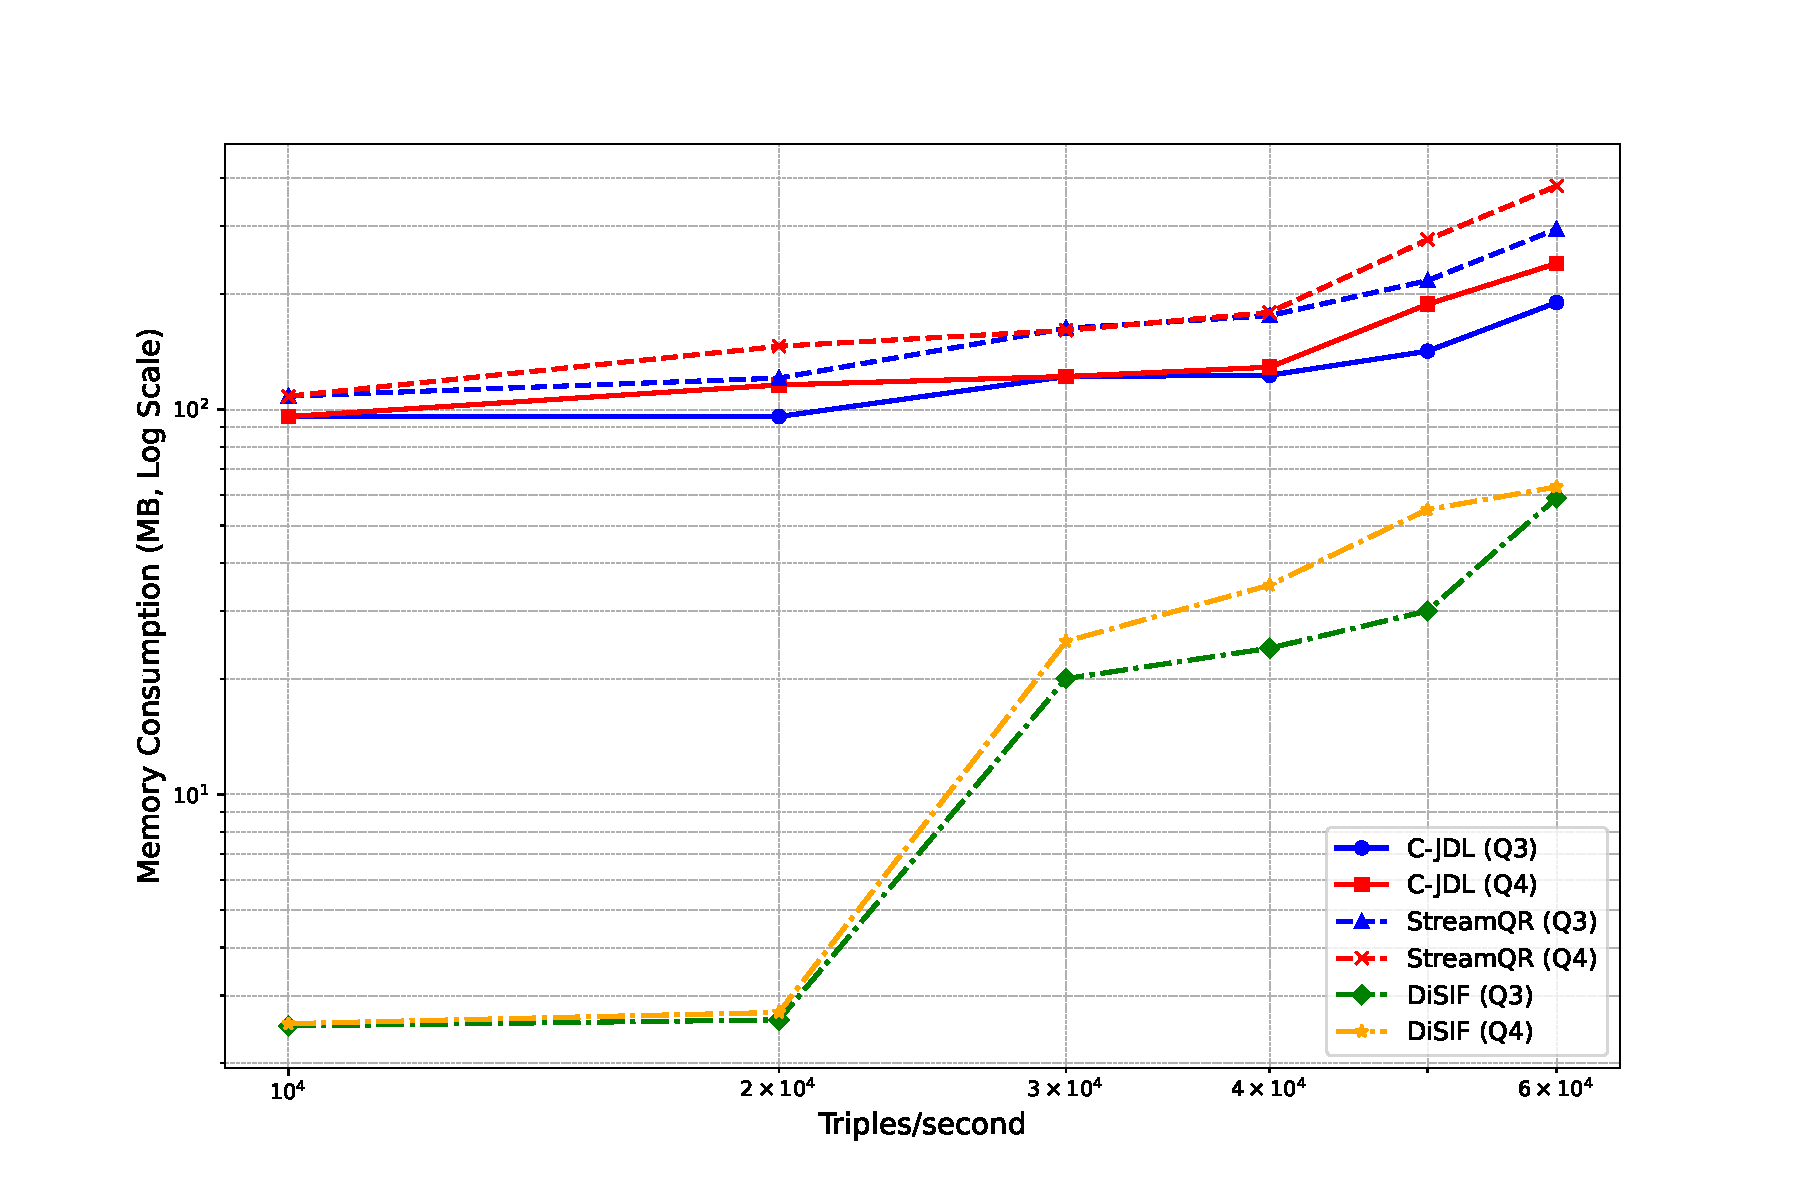
\includegraphics[width=0.8\columnwidth]{Memory_Consumption_vs_Stream_Rate_Log_Enhanced_Q3Q4.pdf}
  \caption{Memory consumption for a single stream receiver node (Log Scale) for Q3 and Q4}
  \label{fig:Memexperiment22}
\end{figure}
  %=================

% \begin{figure*}
%   \centering
%   \begin{subfigure}{0.45\textwidth}
%     \centering
%     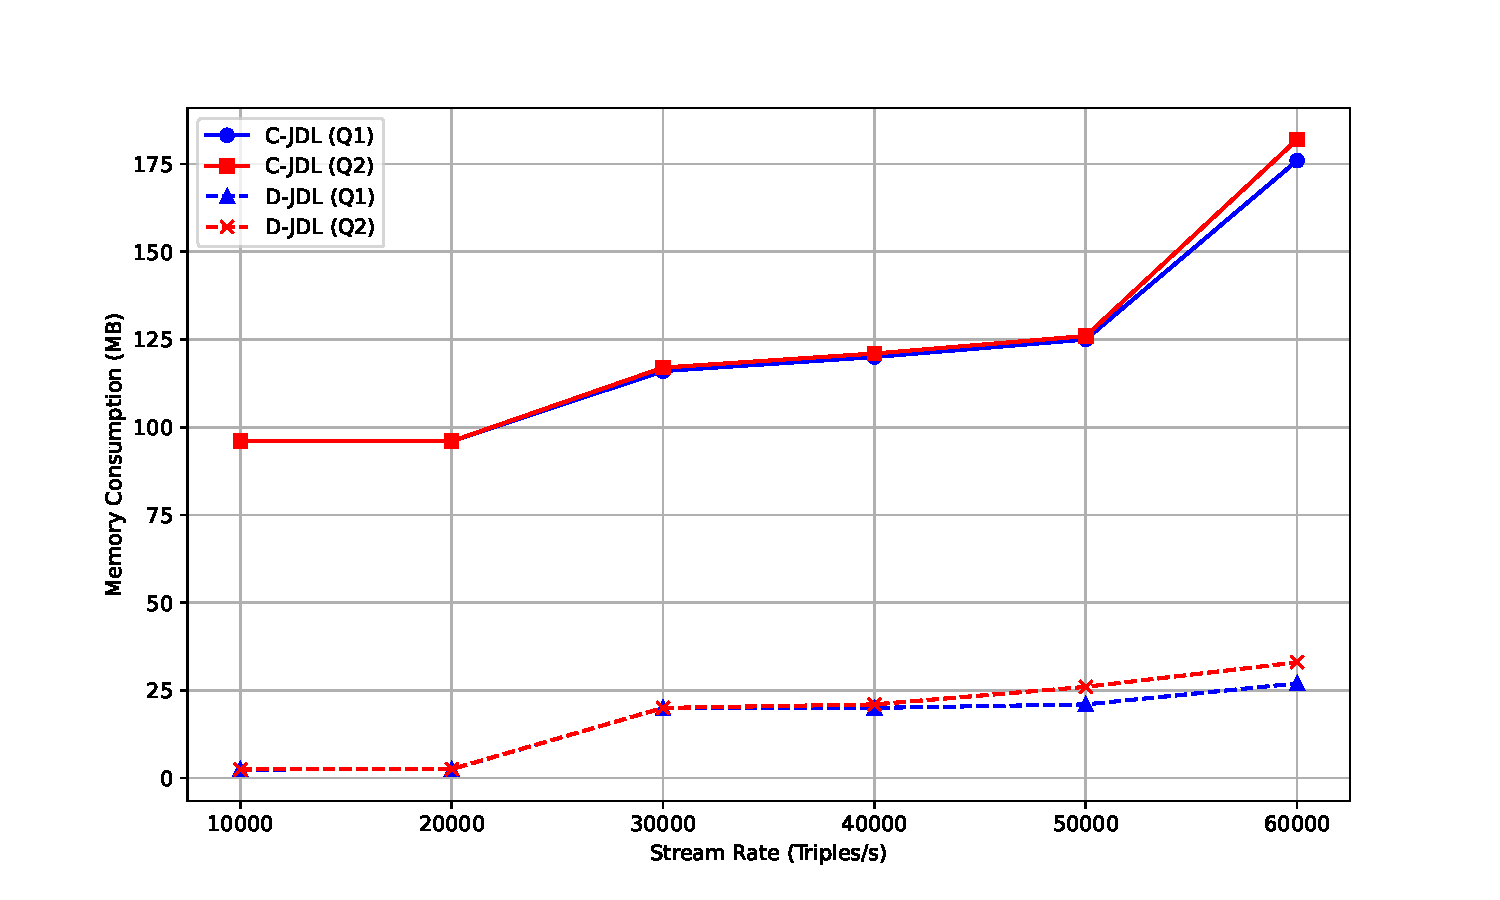
\includegraphics[width=\textwidth]{Memory_Consumption_Q1Q2.pdf}
%     \subcaption{A single stream receiver node}
%     \label{fig:Memexperiment1}
%   \end{subfigure}
%   \hfill
%   \begin{subfigure}{0.45\textwidth}
%     \centering
%     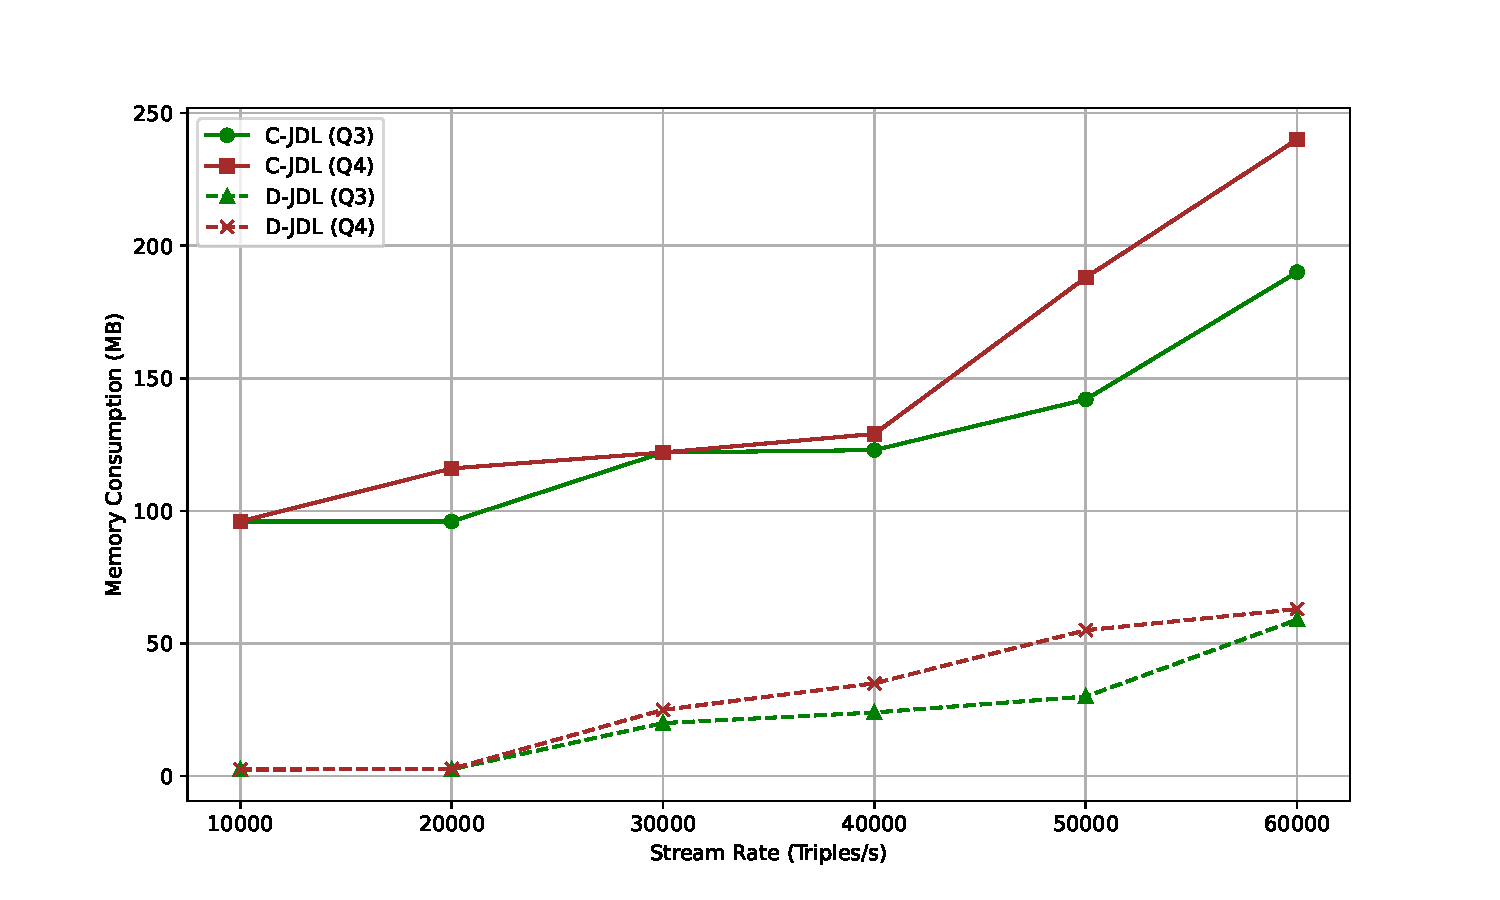
\includegraphics[width=\textwidth]{Memory_Consumption_Q3Q4.pdf}
%     \subcaption{Multiple concurrent stream receiver nodes}
%     \label{fig:Memexperiment2}
%   \end{subfigure}

%   \caption{Memory consumption for different stream reciever nodes}
%   \label{fig:Memexperiment1234}
% \end{figure*}


The StreamQR method, due to the aggregation of queries and the execution of a single
 large query (expanded query), can have higher memory consumption compared
  to the C-JDL method. The execution of this large query may require significant
   memory to process all the input data simultaneously and store intermediate results.
    Managing and processing the aggregated query, along with handling large volumes
     of intermediate data and results, can substantially increase memory usage in StreamQR.


In contrast, the C-JDL method manages memory separately for each query.
 Memory is temporarily released after each query's execution, as memory is only used 
 for the results and processing of individual queries. Despite this, centralized processing
  in C-JDL can still result in high memory usage when handling more complex queries,
   but it is generally lower than StreamQR because queries are executed individually rather
    than aggregated.


As shown in Figures \ref{fig:Memexperiment1} and \ref{fig:Memexperiment11}, memory consumption for executing queries
 $Q_1$ and $Q_2$ in the C-JDL is over four times greater than in
  the DiSIF. This occurs because, in the C-JDL,
   $Q_1$ (or $Q_2$) must be processed to generate outputs stored in the master node's memory,
    which are then used as input for query $Q_m$ to obtain the final results.
     As a result, memory usage in the C-JDL is significantly higher compared to
      the DiSIF.


Query $Q_2$, due to its use of aggregator functions such as GroupBy and Having,
 requires more memory consumption compared to $Q_1$.

On the other hand, Figures \ref{fig:Memexperiment2} and \ref{fig:Memexperiment22}, show that memory consumption
 for queries $Q_3$ and $Q_4$ in C-JDL and StreamQR is significantly higher than 
 in DiSIF approach. This increase is due to the use of AVG functions 
 and CONTAINS, which can elevate memory usage. Storing the outputs in
  memory and then executing $Q_m$ on these outputs substantially increases memory
   consumption for $Q_3$ and $Q_4$ in C-JDL and StreamQR compared
    to DiSIF approach.


Moreover, Figures \ref{fig:Memexperiment1} and \ref{fig:Memexperiment2} demonstrate
 that the AVG and CONTAINS functions in queries $Q_3$ and $Q_4$ can significantly
  increase memory consumption, particularly when data transmission rates exceed 40,000
   triples per second in C-JDL and StreamQR. Additionally, as the data transmission rate
    increases, memory consumption for $Q_4$ surpasses that of $Q_3$, a trend that becomes
     noticeable when data transmission rates surpass 40,000 triples per second.

%\begin{figure}[h]
%    \centering
%    \includegraphics[width=0.8\textwidth]{network_load_comparison.png}
%    \caption{Network Load Comparison}
%\end{figure}
%
%???????????
%# Experiments
%?????????
% \section{Discussion}

\section{Conclusion and future works}
This study introduces a novel distributed semantic JDL fusion model tailored for smart city applications, leveraging a three-layer architecture consisting of edge, fog, and cloud layers. Our framework addresses the limitations of centralized fusion models, particularly the inefficiencies associated with processing vast volumes of heterogeneous data in smart cities. Key benefits of our approach include: 

Enhanced Network Efficiency: By performing low-level data processing at the edge and transmitting only the processed results to higher layers, our model significantly reduces network load and optimizes bandwidth usage.

Reduced Query Execution Time: The ability to decompose complex queries into independent and dependent sub-queries, executed in parallel across different layers, ensures faster query responses and improves overall system responsiveness. 

Improved Data Privacy: Our distributed approach minimizes the need to transmit raw data across the network, thereby enhancing data privacy and security.

Resource Optimization: Distributing computational loads across multiple nodes and layers reduces memory consumption and improves processing efficiency, making the system more scalable and robust.

Our evaluations demonstrate that the distributed JDL model outperforms traditional centralized approaches by reducing network load, decreasing query execution time, and optimizing memory usage. The integration of horizontal and vertical fusion techniques allows for effective management of both heterogeneous and homogeneous data, thus improving the reliability and accuracy of decision-making processes in smart cities.

Furthermore, the DiSIF framework supports real-time, decentralized decision-making, which is critical for addressing the diverse and dynamic needs of urban environments. The innovative approach of combining data fusion at different layers with a distributed query execution model provides a comprehensive solution for the complex data management challenges faced by smart cities.

Future research will focus on refining the model, exploring its application across various smart city scenarios, and addressing new challenges related to large-scale data fusion and real-time processing. The DiSIF framework represents a significant advancement in the efficient management and utilization of smart city data, paving the way for more responsive, adaptive, and intelligent urban systems.

\section{Declaration of competing interest}

The authors declare that they have no known competing financial
interests or personal relationships that could have appeared
to influence the work reported in this paper.

%\section{Data availability}   (mitavanim nadashte bashim)

%\section*{Appendix. Basic graph pattern}

% \section*{Acknowledgments}   (ma nadarim)

% Acknowledgments (if any) go here


%\section{References}

%\bibliographystyle{ieeetr}
%\bibstyle{ieeetr}
\bibliographystyle{plain}

\bibliography{thesis_bib} % Replace 'your_bibliography_file' with the name of your .bib file



% Start the appendix
\appendix

\section{Queries}
\label{sec:AppendixQueries}
% Content of Appendix B


\textbf{Query \(Q_m\)}
\begin{verbatim}
REGISTER QUERY Traffic AS
    PREFIX ex: <http://myexample.org/>
    PREFIX loc: <https://location.com/>
    PREFIX stat: <https://status.com/>
    PREFIX cnt: <https://cntVehicles/>
    PREFIX concept: <https://concept.com/>

    SELECT ?s
    FROM STREAM <streamIRI_new>
                 [RANGE 3s STEP 1s]
    WHERE {
        ?s concept:congestion ?o .
    }
    GROUP BY (?s)
    HAVING (COUNT(?o) > 3);
\end{verbatim}



\textbf{Query 1}

\begin{verbatim}

REGISTER QUERY CongestionDetect AS
PREFIX ex: <http://example.org/>
PREFIX geo: <http://www.w3.org/2003/
            01/geo/wgs84_pos#>
PREFIX stat: <https://status.com/>
PREFIX concept: <https://concept.com/>

CONSTRUCT {
  ?location concept:congestion "congestion" .
}
FROM STREAM <https://www.wtlab.com/TrafficStream>
            [RANGE 3s STEP 1s]
WHERE {
  ?vehicle geo:location ?location ;
           concept:speed ?speedValue ;
           ex:timestamp ?timestamp .
  FILTER(?speed < 50)
}

\end{verbatim}

\textbf{Query 2:}

\begin{verbatim}

    REGISTER QUERY CongestionDetect AS
    PREFIX ex: <http://example.org/>
    PREFIX geo: <http://www.w3.org/2003/01/
                geo/wgs84_pos#>
    PREFIX concept: <https://concept.com/>

    CONSTRUCT {
      ?location concept:congestion "congestion" .
    }
    FROM STREAM <https://www.wtlab.com/TrafficStream>
                 [RANGE 3s STEP 1s]
    WHERE {
      ?vehicle geo:location ?location ;
               concept:speed ?speedValue ;
               ex:timestamp ?timestamp .
      FILTER(?speed < 50)
    }
    GROUP BY ?location
    HAVING (COUNT(?vehicle) > 3)
    ORDER BY ASC(?location)
\end{verbatim}

\textbf{Query 3:}
\begin{verbatim}
REGISTER QUERY CongestionDetect AS
PREFIX ex: <http://example.org/>
PREFIX geo: <http://www.w3.org/2003/01/
            geo/wgs84_pos#>
PREFIX stat: <https://status.com/>
PREFIX concept: <https://concept.com/>

CONSTRUCT {
  ?location concept:congestion "congestion" .
  ?location stat:avgSpeed ?avgLocation .
}
FROM STREAM <https://www.wtlab.com/TrafficStream> 
            [RANGE 3s STEP 1s]
WHERE {
  ?vehicle geo:location ?location ;
           concept:speed ?speedValue ;
           ex:timestamp ?timestamp .

  FILTER(?speed < 50)
  FILTER (CONTAINS(str(?location), "2") ||
          CONTAINS(str(?location), "3") ||
          CONTAINS(str(?location), "1"))
}
GROUP BY ?location
HAVING (COUNT(?vehicle) > 1)
BIND(AVG(?speed) AS ?avgLocation)
ORDER BY ASC(?location)
\end{verbatim}

\textbf{Query 4:}

\begin{verbatim}
REGISTER QUERY CongestionDetect AS
PREFIX ex: <http://example.org/>
PREFIX geo: <http://www.w3.org/2003/01/
            geo/wgs84_pos#>
PREFIX stat: <https://status.com/>
PREFIX concept: <https://concept.com/>

CONSTRUCT {
  ?location concept:congestion "congestion" .
  ?location stat:avgSpeed ?avgLocation .
}
FROM STREAM <https://www.wtlab.com/TrafficStream> 
            [RANGE 3s STEP 1s]
WHERE {
  ?vehicle geo:location ?location ;
           concept:speed ?speedValue ;
           ex:timestamp ?timestamp .

  FILTER(?speed < 50)
  FILTER (CONTAINS(str(?location), "2") ||
          CONTAINS(str(?location), "3") ||
          CONTAINS(str(?location), "1"))
    UNION
    {
    ?vehicle geo:location ?location ;
                ex:speed ?speed ;
                ex:timestamp ?timestamp .
    FILTER(?speed < 50)
    FILTER (CONTAINS(str(?location), "4"))
    }
}
GROUP BY ?location
HAVING (COUNT(?vehicle) > 1)
BIND(AVG(?speed) AS ?avgLocation)
ORDER BY ASC(?location)
\end{verbatim}
\end{document} 